\PassOptionsToPackage{unicode=true}{hyperref} % options for packages loaded elsewhere
\PassOptionsToPackage{hyphens}{url}
%
\documentclass[]{article}
\usepackage{lmodern}
\usepackage{amssymb,amsmath}
\usepackage{ifxetex,ifluatex}
\usepackage{fixltx2e} % provides \textsubscript
\ifnum 0\ifxetex 1\fi\ifluatex 1\fi=0 % if pdftex
  \usepackage[T1]{fontenc}
  \usepackage[utf8]{inputenc}
  \usepackage{textcomp} % provides euro and other symbols
\else % if luatex or xelatex
  \usepackage{unicode-math}
  \defaultfontfeatures{Ligatures=TeX,Scale=MatchLowercase}
\fi
% use upquote if available, for straight quotes in verbatim environments
\IfFileExists{upquote.sty}{\usepackage{upquote}}{}
% use microtype if available
\IfFileExists{microtype.sty}{%
\usepackage[]{microtype}
\UseMicrotypeSet[protrusion]{basicmath} % disable protrusion for tt fonts
}{}
\IfFileExists{parskip.sty}{%
\usepackage{parskip}
}{% else
\setlength{\parindent}{0pt}
\setlength{\parskip}{6pt plus 2pt minus 1pt}
}
\usepackage{hyperref}
\hypersetup{
            pdftitle={Draft: Replication of ``When Do Renters Behave Like Homeowners? High Rent, Price Anxiety, and NIMBYism''},
            pdfauthor={Ruth Zheng},
            pdfborder={0 0 0},
            breaklinks=true}
\urlstyle{same}  % don't use monospace font for urls
\usepackage[margin=1in]{geometry}
\usepackage{color}
\usepackage{fancyvrb}
\newcommand{\VerbBar}{|}
\newcommand{\VERB}{\Verb[commandchars=\\\{\}]}
\DefineVerbatimEnvironment{Highlighting}{Verbatim}{commandchars=\\\{\}}
% Add ',fontsize=\small' for more characters per line
\usepackage{framed}
\definecolor{shadecolor}{RGB}{248,248,248}
\newenvironment{Shaded}{\begin{snugshade}}{\end{snugshade}}
\newcommand{\AlertTok}[1]{\textcolor[rgb]{0.94,0.16,0.16}{#1}}
\newcommand{\AnnotationTok}[1]{\textcolor[rgb]{0.56,0.35,0.01}{\textbf{\textit{#1}}}}
\newcommand{\AttributeTok}[1]{\textcolor[rgb]{0.77,0.63,0.00}{#1}}
\newcommand{\BaseNTok}[1]{\textcolor[rgb]{0.00,0.00,0.81}{#1}}
\newcommand{\BuiltInTok}[1]{#1}
\newcommand{\CharTok}[1]{\textcolor[rgb]{0.31,0.60,0.02}{#1}}
\newcommand{\CommentTok}[1]{\textcolor[rgb]{0.56,0.35,0.01}{\textit{#1}}}
\newcommand{\CommentVarTok}[1]{\textcolor[rgb]{0.56,0.35,0.01}{\textbf{\textit{#1}}}}
\newcommand{\ConstantTok}[1]{\textcolor[rgb]{0.00,0.00,0.00}{#1}}
\newcommand{\ControlFlowTok}[1]{\textcolor[rgb]{0.13,0.29,0.53}{\textbf{#1}}}
\newcommand{\DataTypeTok}[1]{\textcolor[rgb]{0.13,0.29,0.53}{#1}}
\newcommand{\DecValTok}[1]{\textcolor[rgb]{0.00,0.00,0.81}{#1}}
\newcommand{\DocumentationTok}[1]{\textcolor[rgb]{0.56,0.35,0.01}{\textbf{\textit{#1}}}}
\newcommand{\ErrorTok}[1]{\textcolor[rgb]{0.64,0.00,0.00}{\textbf{#1}}}
\newcommand{\ExtensionTok}[1]{#1}
\newcommand{\FloatTok}[1]{\textcolor[rgb]{0.00,0.00,0.81}{#1}}
\newcommand{\FunctionTok}[1]{\textcolor[rgb]{0.00,0.00,0.00}{#1}}
\newcommand{\ImportTok}[1]{#1}
\newcommand{\InformationTok}[1]{\textcolor[rgb]{0.56,0.35,0.01}{\textbf{\textit{#1}}}}
\newcommand{\KeywordTok}[1]{\textcolor[rgb]{0.13,0.29,0.53}{\textbf{#1}}}
\newcommand{\NormalTok}[1]{#1}
\newcommand{\OperatorTok}[1]{\textcolor[rgb]{0.81,0.36,0.00}{\textbf{#1}}}
\newcommand{\OtherTok}[1]{\textcolor[rgb]{0.56,0.35,0.01}{#1}}
\newcommand{\PreprocessorTok}[1]{\textcolor[rgb]{0.56,0.35,0.01}{\textit{#1}}}
\newcommand{\RegionMarkerTok}[1]{#1}
\newcommand{\SpecialCharTok}[1]{\textcolor[rgb]{0.00,0.00,0.00}{#1}}
\newcommand{\SpecialStringTok}[1]{\textcolor[rgb]{0.31,0.60,0.02}{#1}}
\newcommand{\StringTok}[1]{\textcolor[rgb]{0.31,0.60,0.02}{#1}}
\newcommand{\VariableTok}[1]{\textcolor[rgb]{0.00,0.00,0.00}{#1}}
\newcommand{\VerbatimStringTok}[1]{\textcolor[rgb]{0.31,0.60,0.02}{#1}}
\newcommand{\WarningTok}[1]{\textcolor[rgb]{0.56,0.35,0.01}{\textbf{\textit{#1}}}}
\usepackage{longtable,booktabs}
% Fix footnotes in tables (requires footnote package)
\IfFileExists{footnote.sty}{\usepackage{footnote}\makesavenoteenv{longtable}}{}
\usepackage{graphicx,grffile}
\makeatletter
\def\maxwidth{\ifdim\Gin@nat@width>\linewidth\linewidth\else\Gin@nat@width\fi}
\def\maxheight{\ifdim\Gin@nat@height>\textheight\textheight\else\Gin@nat@height\fi}
\makeatother
% Scale images if necessary, so that they will not overflow the page
% margins by default, and it is still possible to overwrite the defaults
% using explicit options in \includegraphics[width, height, ...]{}
\setkeys{Gin}{width=\maxwidth,height=\maxheight,keepaspectratio}
\setlength{\emergencystretch}{3em}  % prevent overfull lines
\providecommand{\tightlist}{%
  \setlength{\itemsep}{0pt}\setlength{\parskip}{0pt}}
\setcounter{secnumdepth}{5}
% Redefines (sub)paragraphs to behave more like sections
\ifx\paragraph\undefined\else
\let\oldparagraph\paragraph
\renewcommand{\paragraph}[1]{\oldparagraph{#1}\mbox{}}
\fi
\ifx\subparagraph\undefined\else
\let\oldsubparagraph\subparagraph
\renewcommand{\subparagraph}[1]{\oldsubparagraph{#1}\mbox{}}
\fi

% set default figure placement to htbp
\makeatletter
\def\fps@figure{htbp}
\makeatother

\usepackage{dcolumn}
\usepackage{float}

\title{Draft: Replication of ``When Do Renters Behave Like Homeowners? High Rent, Price Anxiety, and NIMBYism''}
\author{Ruth Zheng}
\date{April 24, 2020}

\begin{document}
\maketitle

\hypertarget{abstract}{%
\section{Abstract}\label{abstract}}

Hankinson (2018) shows that renters exhibit ``Not in My Back Yard'' (NIMBY) behavior on par with homeowners in high-rent cities despite overall support for a housing supply increase. I successfully replicated Hankinson's results. The increased likelihood for these renters to reject policy proposals that create new housing helps explain the affordable housing crisis in major American cities.

\hypertarget{introduction}{%
\section{Introduction}\label{introduction}}

Using original data sets from an exit poll in San Francisco and a nation-wide survey, Hankinson shows that renters are more likely to exhibit NIMBY-ism when they live in high density cities with high price levels controlling for other demographic characteristics -- hankinson demonstrates this statistically significant and positive relationship between neighborhood price levels and two response variables: one indicating opposition to a housing supply increase and the other support for a ban on neighborhood development in both ``ordinary'' data sets and a set from a nation-wide conjoint survey. The data also confirms the prevailing assumption that renters are more likely to support housing supply increases in general. Hankinson reasons a causal mechanism for this surprising trend may be that renters in high-rent neighborhoods fear that new housing may spur gentrification which would only further drive rent up. Exploring this hypothesis, he shows a significant and positive relationship between housing price-related anxiety and renters' likelihood for exhibiting NIMBY-ism.

\hypertarget{literature-review}{%
\section{Literature Review}\label{literature-review}}

In the past 30 years, the housing market has seen a trend of widening inequality (Glaeser, Gyourko, and Saks 2005). Prices in the top quintile have dramatically increased, particularly in crowded, ``superstar'' cities such as San Francisco, New York City, and Los Angeles. Yet, the resulting housing shortage cannot be attributed to a natural supply ceiling alone (Glaeser, Gyourko, and Saks 2008; Solnit and Schwartzenberg 2000). Glaeser and Gyourko find that in Manhattan prices are twice their supply costs (Glaeser, Gyourko, and Saks 2008). Likewise, Barton demonstrates that in San Francisco, high rents cannot be accounted for by higher real value -- that is, quality, operating costs, and construction costs (Barton 2011). They argue that the decoupling of supply and demand in Manhattan and other major cities must be attributed at least in part to regulation constraining the housing supply (Glaeser, Gyourko, and Saks 2008). Specifically, land-use regulations are associated with reductions in construction activity and higher prices (Glaeser and Ward 2008; Ilhanfeldt 2007). In fact, the responsiveness of the housing supply to increased demand seems to depend significantly on land use and planning regulations (Caldera and Johansson 2013). This is particularly true in high-price locales such as the greater Boston area (Glaeser and Ward 2008) and the San Francisco Bay Area (Kok, Monkkonen, and Quigley 2014).

It is generally accepted that homeowners have an incentive to support regulations that raise the value of their homes (Glaeser, Gyourko, and Saks 2005; Quigley and Rosenthal 2005; Rohe and Stewart 1996). Typically higher income homeowners are the ones who dominate local politics underlying land use enactments (Quigley and Rosenthal 2005). On the other hand, renters, who usually want lower prices, are expected to support policies and public spending that favor constructing new housing (Brunner, Ross, and Simonsen 2015; Desmond 2017). However, this dynamic cannot entirely explain persistent supply-discouraging regulations in major cities where homeownership rates are lower and pale in comparison to renters.

Hankinson hypothesizes that in high-rent cities, renters adopt a form of ``Not in My Back Yard-ism'' (NIMBY-ism). This would give rise to a collective action problem in the political-economy of local housing wherein despite supporting city-wide housing supply increases and other policies favoring affordable housing, renters oppose such policies in their own neighborhoods. As a result, no neighborhood is politically willing to bear the cost of new housing. While there is a rich existing literature on NIMBY-ism among homeowners (Dear 1992; Schively 2007), there has been comparatively little research done on the appearance of this behavior among renters (Fischel 2000). In fact, renters are expected to exhibit lower levels of NIMBY-ism as the ephemerality of renting means they have less of a stake in the good or bad things that happen in their neighborhoods (Moomau and Morton 1992). Renters' behavior in high-rent cities demands closer examination. What is driving renters to continue to enact housing regulations? And, what external and/or demographic factors cause renters policy behavior to become sensitive to the proximity of proposed new housing?

\hypertarget{replication}{%
\section{Replication}\label{replication}}

Hankinson's original paper includes 27 figures. I have replicated 21 of them. Those that I have not replicated are mainly clarifying tables, that is they include summary statistics, demonstrate theoretical results, or attempt to illustrate a hypothetical example. I chose not to replicate these tables because they do not directly pertain to the actual analysis of Hankinson's data set and thus do not contribute to answering the research question about what factors are associated with renters exhibiting NIMBY behavior.

\hypertarget{extension}{%
\section{Extension}\label{extension}}

I extend Hankinson's analysis by using logistic regression to refit three sets of models: the first set (table A.3) regresses an indicator variable for supporting a 10 \% housing supply increase and one for supporting a NIMBY ban onto homeownership status including demographic controls and fixed effects for the San Francisco data set; the second (table B.2) regresses an indicator for supporting a 10\% supply increase onto homeownership status including demographics and fixed effects for the natiowide data set; the third (table B.4) regresses an indicator for supporting a ban on neighborhood development (NIMBY ban) on homeownership status including demographic controls and fixed effects for the nationwide data set. While Hankinson fits ordinary least squares models, likely for ease of comparison, this risks violating normality of errors and allows the response variable to exceed the scope of 0 and 1 which breaks probability axioms. A logistic regression can better model a range of probabilities using the logistic function which is strictly between 0 and 1.

The logistic output for the first set of regressions (table A.3) showed a consistently negative relationship between homeownership and both the probability of supporting a 10\% supply increase and for supporting a NIMBY ban. Using the divide by four rule, holding all else constant, homeowners are about 10\% less likely to support both the supply increase and the neighborhood ban than renters. These estimates, however, are not statistically significant. This is consistent with the OLS model which outputs a weak and consistently negative coefficients on homeownership status. The logistic output for the second set of regressions (table B.2) showed a consistently negative and statistically insignificant relationship between homeownership status and probability of supporting a 10\% supply increase. Using the divide by four rule, the logistic regression estimates that holding all else constant homeowners are at most 25\% less likely to support the increase. Although these estimates are constitent in sign and magnitude with the OLS estimates, the OLS coefficients are statistically significant. Finally, the logistic output for the third set of regressions (table B.4) showed a consistently positive and, once again, statistically insignificant relationship between homeownership and probability of supporting a ban on neighborhood development. Holding all else constant, homeowners are at most 7.5\%. more likely to support the ban than renters. This is again consistent with the OLS results with the primary difference being that the OLS coefficients are statistically significant at the \(\alpha = .05\) level.

These results confirm the puzzle Hankinson attempts to elucidate: despite an overall tendency for homeowners to be more likely than renters to exhibit NIMBY behavior, why do renters seem to demonstrate NIMBY-ism on par with, if not even more than, homeowners in a housing market like that of San Francisco?

\hypertarget{table-a.3-extension-policy-proposals-san-francisco-sample-logistic}{%
\subsection{Table A.3 Extension Policy Proposals, San Francisco Sample Logistic}\label{table-a.3-extension-policy-proposals-san-francisco-sample-logistic}}

\% Table created by stargazer v.5.2.2 by Marek Hlavac, Harvard University. E-mail: hlavac at fas.harvard.edu
\% Date and time: Sat, Apr 25, 2020 - 00:40:44
\% Requires LaTeX packages: dcolumn

\begin{table}[H] \centering 
  \caption{Policy Proposals, San Francisco Sample} 
  \label{sf_policies} 
\small 
\begin{tabular}{@{\extracolsep{5pt}}lD{.}{.}{-2} D{.}{.}{-2} D{.}{.}{-2} D{.}{.}{-2} } 
\\[-1.8ex]\hline 
\hline \\[-1.8ex] 
 & \multicolumn{4}{c}{\textit{Dependent variable:}} \\ 
\cline{2-5} 
 & \multicolumn{2}{c}{10 Pct Supply} & \multicolumn{2}{c}{NIMBY Ban Proposal} \\ 
\\[-1.8ex] & \multicolumn{1}{c}{(1)} & \multicolumn{1}{c}{(2)} & \multicolumn{1}{c}{(3)} & \multicolumn{1}{c}{(4)}\\ 
\hline \\[-1.8ex] 
 Homeownership & -.41 & -.40 & -.88 & -.42 \\ 
  & (.12) & (.46) & (.12) & (.17) \\ 
  Ideology &  & .36 &  & .47 \\ 
  &  & (.18) &  & (.08) \\ 
  Income, Log &  & .36 &  & -.62 \\ 
  &  & (.21) &  & (.08) \\ 
  White, Non-Hispanic &  & .39 &  & -.48 \\ 
  &  & (.36) &  & (.15) \\ 
  Age &  & -.01 &  & .02 \\ 
  &  & (.01) &  & (.01) \\ 
  Male &  & .52 &  & -.43 \\ 
  &  & (.35) &  & (.14) \\ 
  Constant & .51 & 1.89 & .47 & .22 \\ 
  & (.07) & (.61) & (.07) & (.24) \\ 
 \hline \\[-1.8ex] 
Observations & \multicolumn{1}{c}{1,175} & \multicolumn{1}{c}{270} & \multicolumn{1}{c}{1,294} & \multicolumn{1}{c}{1,087} \\ 
Log Likelihood & \multicolumn{1}{c}{-790.31} & \multicolumn{1}{c}{-111.15} & \multicolumn{1}{c}{-865.38} & \multicolumn{1}{c}{-649.94} \\ 
Akaike Inf. Crit. & \multicolumn{1}{c}{1,584.62} & \multicolumn{1}{c}{236.30} & \multicolumn{1}{c}{1,734.76} & \multicolumn{1}{c}{1,313.89} \\ 
\hline 
\hline \\[-1.8ex] 
\end{tabular} 
\end{table}

\% Table created by stargazer v.5.2.2 by Marek Hlavac, Harvard University. E-mail: hlavac at fas.harvard.edu
\% Date and time: Sat, Apr 25, 2020 - 00:40:44
\% Requires LaTeX packages: dcolumn

\begin{table}[H] \centering 
  \caption{Policy Proposals, San Francisco Sample} 
  \label{sf_policies} 
\small 
\begin{tabular}{@{\extracolsep{5pt}} D{.}{.}{-2} } 
\\[-1.8ex]\hline 
\hline \\[-1.8ex] 
\multicolumn{1}{c}{} \\ 
\hline \\[-1.8ex] 
\end{tabular} 
\end{table}

\hypertarget{extension-of-table-b.2.-support-for-10-supply-increase}{%
\subsection{Extension of table B.2. Support for 10\% Supply Increase}\label{extension-of-table-b.2.-support-for-10-supply-increase}}

\begin{verbatim}
## Warning in sqrt(diag(vcovHC(supply_full_fe, type = "HC1"))): NaNs produced
\end{verbatim}

\% Table created by stargazer v.5.2.2 by Marek Hlavac, Harvard University. E-mail: hlavac at fas.harvard.edu
\% Date and time: Fri, Apr 24, 2020 - 23:59:41
\% Requires LaTeX packages: dcolumn

\begin{table}[H] \centering 
  \caption{Support for 10 Percent Supply Increase} 
  \label{supply_7} 
\small 
\begin{tabular}{@{\extracolsep{5pt}}lD{.}{.}{-2} D{.}{.}{-2} D{.}{.}{-2} } 
\\[-1.8ex]\hline 
\hline \\[-1.8ex] 
 & \multicolumn{1}{c}{Bivariate} & \multicolumn{1}{c}{Full} & \multicolumn{1}{c}{Full with Fixed Effects} \\ 
\\[-1.8ex] & \multicolumn{1}{c}{(1)} & \multicolumn{1}{c}{(2)} & \multicolumn{1}{c}{(3)}\\ 
\hline \\[-1.8ex] 
 Homeownership & -1.32 & -1.08 & -1.03 \\ 
  & (.10) & (.12) & (.19) \\ 
  Ideology &  & .21 & .24 \\ 
  &  & (.05) & (.08) \\ 
  Income, Log &  & -.10 & -.09 \\ 
  &  & (.06) & (.09) \\ 
  White, Non-Hispanic &  & -.41 & -.41 \\ 
  &  & (.11) & (.17) \\ 
  Age &  & -.01 & -.01 \\ 
  &  & (.003) & (.01) \\ 
  Male &  & .29 & .33 \\ 
  &  & (.11) & (.16) \\ 
  Constant & .35 & .57 & -17.01 \\ 
  & (.08) & (.18) &  \\ 
 \hline \\[-1.8ex] 
Observations & \multicolumn{1}{c}{1,909} & \multicolumn{1}{c}{1,878} & \multicolumn{1}{c}{1,878} \\ 
Log Likelihood & \multicolumn{1}{c}{-1,177.17} & \multicolumn{1}{c}{-1,133.75} & \multicolumn{1}{c}{-810.21} \\ 
Akaike Inf. Crit. & \multicolumn{1}{c}{2,358.34} & \multicolumn{1}{c}{2,281.51} & \multicolumn{1}{c}{2,678.41} \\ 
\hline 
\hline \\[-1.8ex] 
\end{tabular} 
\end{table}

\hypertarget{extension-of-table-b.3-support-for-10-supply-increaseseven-point-scale}{%
\subsection{Extension of table B.3 Support for 10\% Supply Increase---Seven-Point Scale}\label{extension-of-table-b.3-support-for-10-supply-increaseseven-point-scale}}

\hypertarget{extension-of-table-b.4-support-for-ban-on-neighborhood-development}{%
\subsection{Extension of table B.4 Support for Ban on Neighborhood Development}\label{extension-of-table-b.4-support-for-ban-on-neighborhood-development}}

\begin{verbatim}
## Warning in sqrt(diag(vcovHC(ban_full_fe, type = "HC1"))): NaNs produced
\end{verbatim}

\% Table created by stargazer v.5.2.2 by Marek Hlavac, Harvard University. E-mail: hlavac at fas.harvard.edu
\% Date and time: Sat, Apr 25, 2020 - 00:11:39
\% Requires LaTeX packages: dcolumn

\begin{table}[H] \centering 
  \caption{Support for Ban on Neighborhood Development} 
  \label{ban_dummy} 
\small 
\begin{tabular}{@{\extracolsep{5pt}}lD{.}{.}{-2} D{.}{.}{-2} D{.}{.}{-2} } 
\\[-1.8ex]\hline 
\hline \\[-1.8ex] 
 & \multicolumn{1}{c}{Bivariate} & \multicolumn{1}{c}{Full} & \multicolumn{1}{c}{Full with Fixed Effects} \\ 
\\[-1.8ex] & \multicolumn{1}{c}{(1)} & \multicolumn{1}{c}{(2)} & \multicolumn{1}{c}{(3)}\\ 
\hline \\[-1.8ex] 
 Homeownership & .30 & .30 & .40 \\ 
  & (.10) & (.11) & (.17) \\ 
  Ideology &  & -.14 & -.14 \\ 
  &  & (.05) & (.07) \\ 
  Income, Log &  & -.003 & -.04 \\ 
  &  & (.05) & (.08) \\ 
  White, Non-Hispanic &  & -.16 & -.23 \\ 
  &  & (.10) & (.16) \\ 
  Age &  & .002 & .002 \\ 
  &  & (.003) & (.004) \\ 
  Male &  & -.11 & -.08 \\ 
  &  & (.09) & (.14) \\ 
  Constant & -.62 & -.60 & -18.95 \\ 
  & (.08) & (.16) &  \\ 
 \hline \\[-1.8ex] 
Observations & \multicolumn{1}{c}{2,072} & \multicolumn{1}{c}{2,032} & \multicolumn{1}{c}{2,032} \\ 
Log Likelihood & \multicolumn{1}{c}{-1,388.80} & \multicolumn{1}{c}{-1,354.09} & \multicolumn{1}{c}{-984.42} \\ 
Akaike Inf. Crit. & \multicolumn{1}{c}{2,781.61} & \multicolumn{1}{c}{2,722.19} & \multicolumn{1}{c}{3,084.83} \\ 
\hline 
\hline \\[-1.8ex] 
\end{tabular} 
\end{table}

\hypertarget{extension-of-table-b.5-support-for-ban-on-neighborhood-developmentseven-point-scale}{%
\subsection{Extension of table B.5 Support for Ban on Neighborhood Development---Seven-Point Scale}\label{extension-of-table-b.5-support-for-ban-on-neighborhood-developmentseven-point-scale}}

\hypertarget{replication-results}{%
\section{Replication Results}\label{replication-results}}

\hypertarget{figure-1.-support-for-a-neighborhood-ban-on-new-development-by-support-for-a-10-increase-in-the-citys-housing-supply}{%
\subsubsection{Figure 1. Support for a Neighborhood Ban on New Development by Support for a 10\% Increase in the City's Housing Supply}\label{figure-1.-support-for-a-neighborhood-ban-on-new-development-by-support-for-a-10-increase-in-the-citys-housing-supply}}

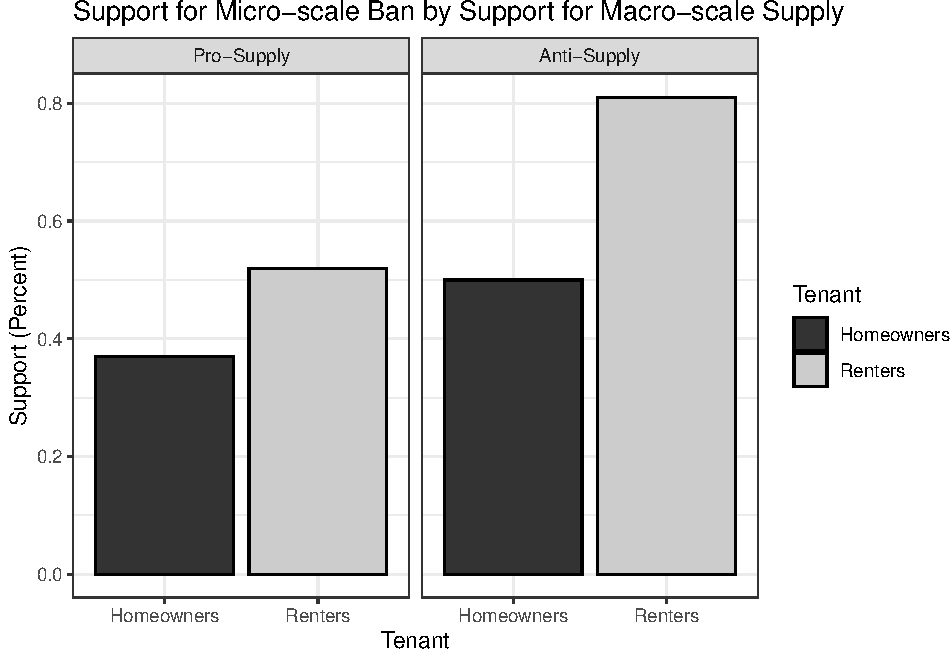
\includegraphics{Zheng-Ruth-Renters-Paper_files/figure-latex/Figure 1-1.pdf}

\hypertarget{figure-3.-effect-of-proximity-on-homeowners-by-affordability-of-proposed-housing}{%
\subsubsection{Figure 3. Effect of Proximity on Homeowners by Affordability of Proposed Housing}\label{figure-3.-effect-of-proximity-on-homeowners-by-affordability-of-proposed-housing}}

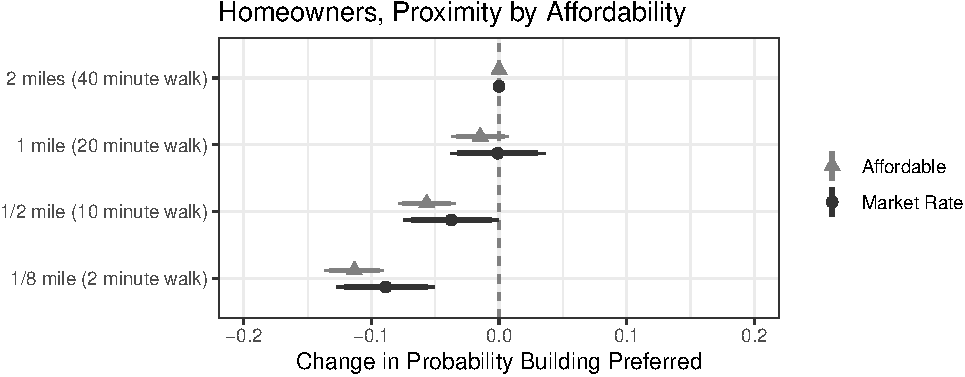
\includegraphics{Zheng-Ruth-Renters-Paper_files/figure-latex/Figure 3 print-1.pdf}

\hypertarget{figure-4-effect-of-proximity-on-renters-by-affordability-of-proposed-housing}{%
\subsubsection{Figure 4 Effect of Proximity on Renters by Affordability of Proposed Housing}\label{figure-4-effect-of-proximity-on-renters-by-affordability-of-proposed-housing}}

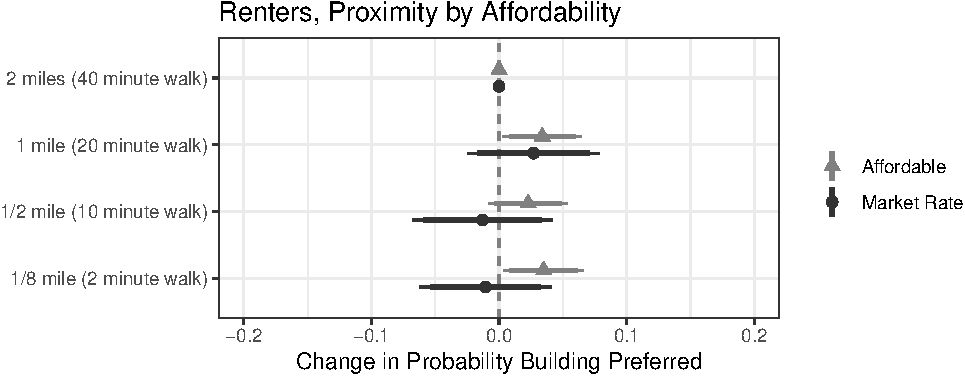
\includegraphics{Zheng-Ruth-Renters-Paper_files/figure-latex/Figure 4-1.pdf}

\hypertarget{figure-5-effect-of-proximity-on-renters-by-affordability-of-proposed-housing-grouped-by-average-rent-citywide.-displayed-effect-is-shift-from-two-miles-away-baseline-to-an-eighth-of-a-mile-away.-quintile-cutpoints-for-average-rent-by-city-at-1217-1480-1936-and-2247}{%
\subsubsection{Figure 5 Effect of Proximity on Renters by Affordability of Proposed Housing, Grouped by Average Rent Citywide. Displayed Effect is Shift from Two Miles Away (Baseline) to an Eighth of a Mile Away. Quintile Cutpoints for Average Rent by City at \$1,217, \$1,480, \$1,936, and \$2,247}\label{figure-5-effect-of-proximity-on-renters-by-affordability-of-proposed-housing-grouped-by-average-rent-citywide.-displayed-effect-is-shift-from-two-miles-away-baseline-to-an-eighth-of-a-mile-away.-quintile-cutpoints-for-average-rent-by-city-at-1217-1480-1936-and-2247}}

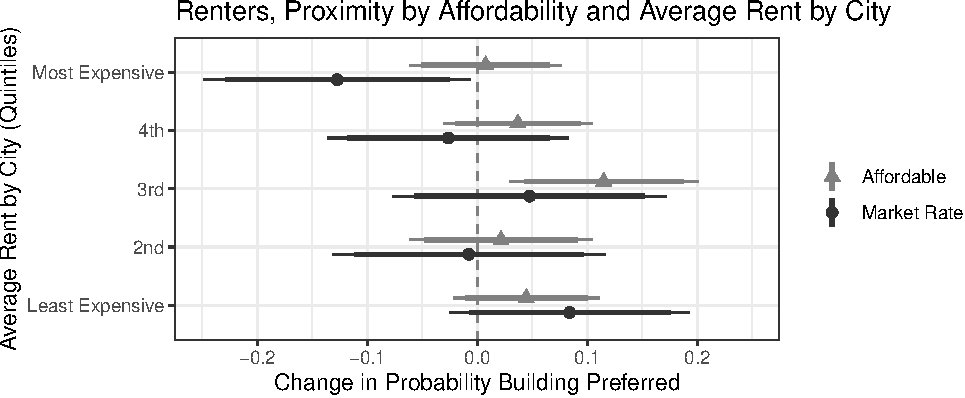
\includegraphics{Zheng-Ruth-Renters-Paper_files/figure-latex/Print Figure 5-1.pdf}

\hypertarget{figure-6.-renter-support-for-a-10-increase-in-their-citytowns-housing-supply-by-average-rent-citywide}{%
\subsubsection{Figure 6. Renter Support for a 10\% Increase in Their City/Town's Housing Supply, by Average Rent Citywide}\label{figure-6.-renter-support-for-a-10-increase-in-their-citytowns-housing-supply-by-average-rent-citywide}}

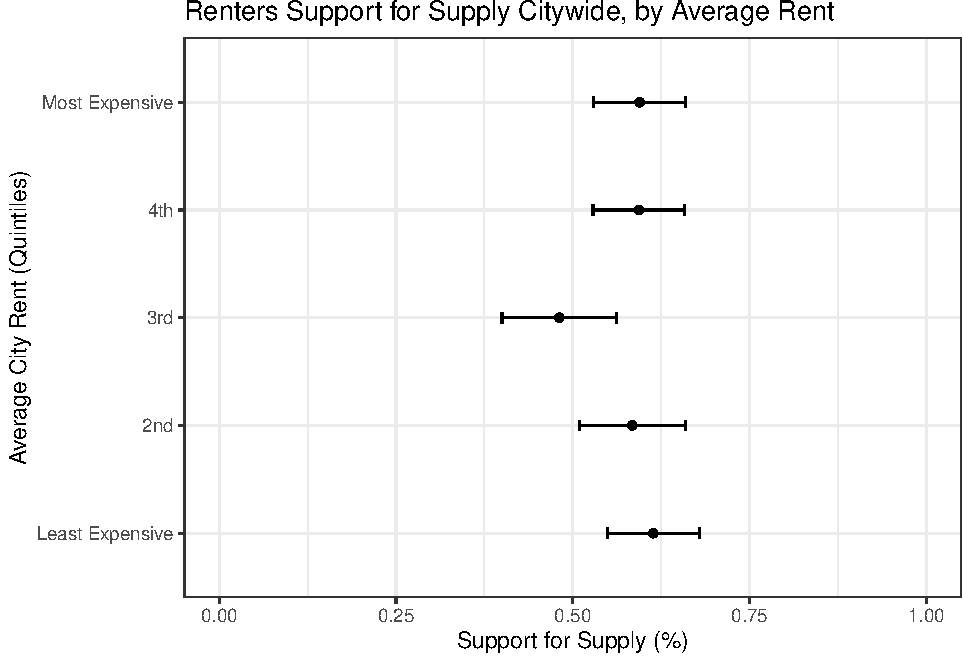
\includegraphics{Zheng-Ruth-Renters-Paper_files/figure-latex/Print Figure 6-1.pdf}

\hypertarget{figure-7.-figure-7.-effect-of-proximity-on-renters-toward-market-rate-housing-by-attitude-toward-housing-prices-citywide}{%
\subsubsection{Figure 7. FIGURE 7. Effect of Proximity on Renters Toward Market-Rate Housing by Attitude Toward Housing Prices Citywide}\label{figure-7.-figure-7.-effect-of-proximity-on-renters-toward-market-rate-housing-by-attitude-toward-housing-prices-citywide}}

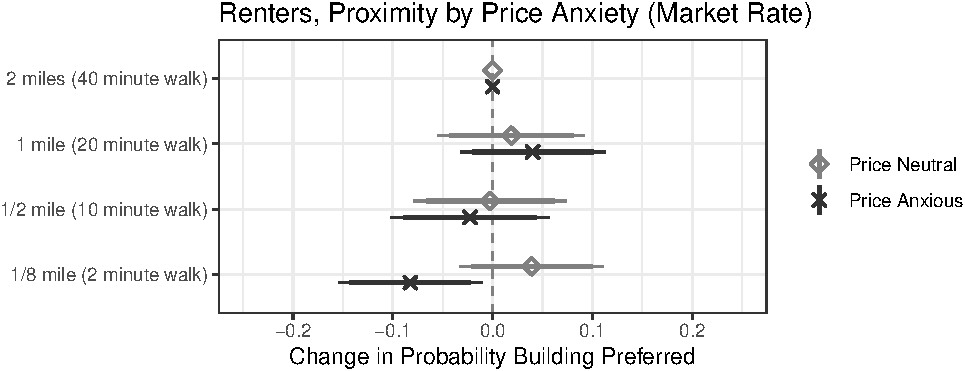
\includegraphics{Zheng-Ruth-Renters-Paper_files/figure-latex/Figure 7 print-1.pdf}

\hypertarget{a-san-francisco}{%
\subsection{A San Francisco}\label{a-san-francisco}}

\hypertarget{table-a.3.-policy-proposals-san-francisco-sample}{%
\subsubsection{Table A.3. Policy Proposals, San Francisco Sample}\label{table-a.3.-policy-proposals-san-francisco-sample}}

\% Table created by stargazer v.5.2.2 by Marek Hlavac, Harvard University. E-mail: hlavac at fas.harvard.edu
\% Date and time: Sat, Apr 25, 2020 - 00:40:50
\% Requires LaTeX packages: dcolumn

\begin{table}[H] \centering 
  \caption{Policy Proposals, San Francisco Sample} 
  \label{sf_policies} 
\small 
\begin{tabular}{@{\extracolsep{5pt}}lD{.}{.}{-2} D{.}{.}{-2} D{.}{.}{-2} D{.}{.}{-2} } 
\\[-1.8ex]\hline 
\hline \\[-1.8ex] 
 & \multicolumn{4}{c}{\textit{Dependent variable:}} \\ 
\cline{2-5} 
 & \multicolumn{2}{c}{10 Pct Supply} & \multicolumn{2}{c}{NIMBY Ban Proposal} \\ 
\\[-1.8ex] & \multicolumn{1}{c}{(1)} & \multicolumn{1}{c}{(2)} & \multicolumn{1}{c}{(3)} & \multicolumn{1}{c}{(4)}\\ 
\hline \\[-1.8ex] 
 Homeownership & -.10 & -.05 & -.22 & -.09 \\ 
  & (.03) & (.06) & (.03) & (.04) \\ 
  Ideology &  & .05 &  & .10 \\ 
  &  & (.03) &  & (.01) \\ 
  Income, Log &  & .05 &  & -.13 \\ 
  &  & (.03) &  & (.02) \\ 
  White, Non-Hispanic &  & .05 &  & -.10 \\ 
  &  & (.05) &  & (.03) \\ 
  Age &  & -.002 &  & .003 \\ 
  &  & (.002) &  & (.001) \\ 
  Male &  & .07 &  & -.09 \\ 
  &  & (.05) &  & (.03) \\ 
  Constant & .62 & .86 & .62 & .55 \\ 
  & (.02) & (.08) & (.02) & (.05) \\ 
 \hline \\[-1.8ex] 
Observations & \multicolumn{1}{c}{1,175} & \multicolumn{1}{c}{270} & \multicolumn{1}{c}{1,294} & \multicolumn{1}{c}{1,087} \\ 
R$^{2}$ & \multicolumn{1}{c}{.01} & \multicolumn{1}{c}{.07} & \multicolumn{1}{c}{.04} & \multicolumn{1}{c}{.17} \\ 
Adjusted R$^{2}$ & \multicolumn{1}{c}{.01} & \multicolumn{1}{c}{.05} & \multicolumn{1}{c}{.04} & \multicolumn{1}{c}{.17} \\ 
\hline 
\hline \\[-1.8ex] 
\end{tabular} 
\end{table}

\% Table created by stargazer v.5.2.2 by Marek Hlavac, Harvard University. E-mail: hlavac at fas.harvard.edu
\% Date and time: Sat, Apr 25, 2020 - 00:40:50
\% Requires LaTeX packages: dcolumn

\begin{table}[H] \centering 
  \caption{Policy Proposals, San Francisco Sample} 
  \label{sf_policies} 
\small 
\begin{tabular}{@{\extracolsep{5pt}} D{.}{.}{-2} } 
\\[-1.8ex]\hline 
\hline \\[-1.8ex] 
\multicolumn{1}{c}{} \\ 
\hline \\[-1.8ex] 
\end{tabular} 
\end{table}

\hypertarget{figure-a.1.-effect-of-proximity-on-recontacted-san-francisco-renters-toward-market-rate-housing-by-support-for-hypothetical-ban-on-market-rate-housing-in-own-neighborhood}{%
\subsubsection{Figure A.1. Effect of Proximity on Recontacted San Francisco Renters Toward Market-Rate Housing by Support for Hypothetical Ban on Market-Rate Housing in own Neighborhood}\label{figure-a.1.-effect-of-proximity-on-recontacted-san-francisco-renters-toward-market-rate-housing-by-support-for-hypothetical-ban-on-market-rate-housing-in-own-neighborhood}}

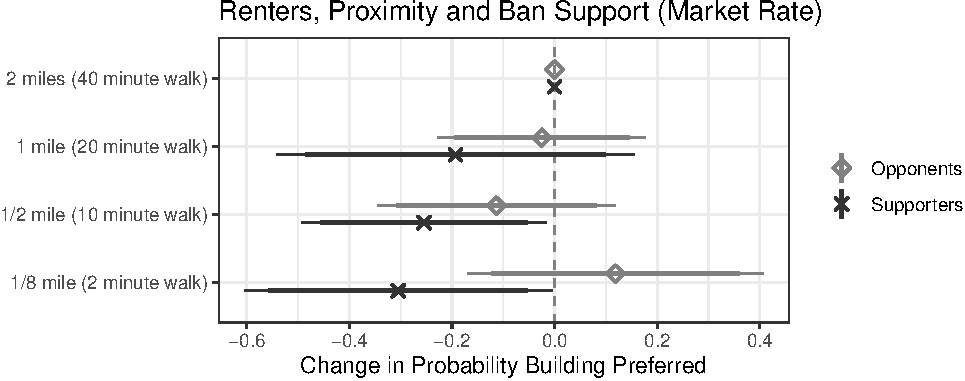
\includegraphics{Zheng-Ruth-Renters-Paper_files/figure-latex/Figure A.1 print-1.pdf}

\hypertarget{national-survey-non-conjoint}{%
\subsection{NATIONAL SURVEY NON-CONJOINT}\label{national-survey-non-conjoint}}

\hypertarget{table-b.2.-support-for-10-supply-increase}{%
\subsubsection{Table B.2. Support for 10\% Supply Increase}\label{table-b.2.-support-for-10-supply-increase}}

\% Table created by stargazer v.5.2.2 by Marek Hlavac, Harvard University. E-mail: hlavac at fas.harvard.edu
\% Date and time: Sat, Apr 25, 2020 - 00:11:50
\% Requires LaTeX packages: dcolumn

\begin{table}[H] \centering 
  \caption{Support for 10 Percent Supply Increase} 
  \label{supply_7} 
\small 
\begin{tabular}{@{\extracolsep{5pt}}lD{.}{.}{-2} D{.}{.}{-2} D{.}{.}{-2} } 
\\[-1.8ex]\hline 
\hline \\[-1.8ex] 
 & \multicolumn{1}{c}{Bivariate} & \multicolumn{1}{c}{Full} & \multicolumn{1}{c}{Full with Fixed Effects} \\ 
\\[-1.8ex] & \multicolumn{1}{c}{(1)} & \multicolumn{1}{c}{(2)} & \multicolumn{1}{c}{(3)}\\ 
\hline \\[-1.8ex] 
 Homeownership & -.31 & -.25 & -.21 \\ 
  & (.02) & (.03) & (.04) \\ 
  Ideology &  & .04 & .04 \\ 
  &  & (.01) & (.01) \\ 
  Income, Log &  & -.02 & -.02 \\ 
  &  & (.01) & (.02) \\ 
  White, Non-Hispanic &  & -.09 & -.08 \\ 
  &  & (.02) & (.03) \\ 
  Age &  & -.001 & -.001 \\ 
  &  & (.001) & (.001) \\ 
  Male &  & .06 & .06 \\ 
  &  & (.02) & (.03) \\ 
  Constant & .59 & .63 & .31 \\ 
  & (.02) & (.04) & (.08) \\ 
 \hline \\[-1.8ex] 
Observations & \multicolumn{1}{c}{1,909} & \multicolumn{1}{c}{1,878} & \multicolumn{1}{c}{1,878} \\ 
R$^{2}$ & \multicolumn{1}{c}{.09} & \multicolumn{1}{c}{.11} & \multicolumn{1}{c}{.36} \\ 
Adjusted R$^{2}$ & \multicolumn{1}{c}{.09} & \multicolumn{1}{c}{.11} & \multicolumn{1}{c}{.11} \\ 
\hline 
\hline \\[-1.8ex] 
\end{tabular} 
\end{table}

\hypertarget{table-b.3.-support-for-10-supply-increaseseven-point-scale}{%
\subsubsection{Table B.3. Support for 10\% Supply Increase---Seven-Point Scale}\label{table-b.3.-support-for-10-supply-increaseseven-point-scale}}

\% Table created by stargazer v.5.2.2 by Marek Hlavac, Harvard University. E-mail: hlavac at fas.harvard.edu
\% Date and time: Sat, Apr 25, 2020 - 00:11:57
\% Requires LaTeX packages: dcolumn

\begin{table}[H] \centering 
  \caption{Support for 10 Percent Supply Increase - 7 Point Scale} 
  \label{supply_7} 
\small 
\begin{tabular}{@{\extracolsep{5pt}}lD{.}{.}{-2} D{.}{.}{-2} D{.}{.}{-2} } 
\\[-1.8ex]\hline 
\hline \\[-1.8ex] 
 & \multicolumn{1}{c}{Bivariate} & \multicolumn{1}{c}{Full} & \multicolumn{1}{c}{Full with Fixed Effects} \\ 
\\[-1.8ex] & \multicolumn{1}{c}{(1)} & \multicolumn{1}{c}{(2)} & \multicolumn{1}{c}{(3)}\\ 
\hline \\[-1.8ex] 
 Homeownership & -.90 & -.69 & -.60 \\ 
  & (.06) & (.07) & (.09) \\ 
  Ideology &  & .13 & .11 \\ 
  &  & (.03) & (.04) \\ 
  Income, Log &  & -.09 & -.07 \\ 
  &  & (.03) & (.04) \\ 
  White, Non-Hispanic &  & -.24 & -.18 \\ 
  &  & (.06) & (.08) \\ 
  Age &  & -.01 & -.01 \\ 
  &  & (.002) & (.002) \\ 
  Male &  & .16 & .15 \\ 
  &  & (.06) & (.07) \\ 
  Constant & 4.20 & 4.44 & 4.08 \\ 
  & (.05) & (.10) & (.20) \\ 
 \hline \\[-1.8ex] 
Observations & \multicolumn{1}{c}{2,902} & \multicolumn{1}{c}{2,846} & \multicolumn{1}{c}{2,846} \\ 
R$^{2}$ & \multicolumn{1}{c}{.07} & \multicolumn{1}{c}{.09} & \multicolumn{1}{c}{.31} \\ 
Adjusted R$^{2}$ & \multicolumn{1}{c}{.07} & \multicolumn{1}{c}{.09} & \multicolumn{1}{c}{.11} \\ 
\hline 
\hline \\[-1.8ex] 
\end{tabular} 
\end{table}

\hypertarget{table-b.4.-support-for-ban-on-neighborhood-development}{%
\subsubsection{Table B.4. Support for Ban on Neighborhood Development}\label{table-b.4.-support-for-ban-on-neighborhood-development}}

\% Table created by stargazer v.5.2.2 by Marek Hlavac, Harvard University. E-mail: hlavac at fas.harvard.edu
\% Date and time: Sat, Apr 25, 2020 - 00:12:02
\% Requires LaTeX packages: dcolumn

\begin{table}[H] \centering 
  \caption{Support for Ban on Neighborhood Development} 
  \label{ban_dummy} 
\small 
\begin{tabular}{@{\extracolsep{5pt}}lD{.}{.}{-2} D{.}{.}{-2} D{.}{.}{-2} } 
\\[-1.8ex]\hline 
\hline \\[-1.8ex] 
 & \multicolumn{1}{c}{Bivariate} & \multicolumn{1}{c}{Full} & \multicolumn{1}{c}{Full with Fixed Effects} \\ 
\\[-1.8ex] & \multicolumn{1}{c}{(1)} & \multicolumn{1}{c}{(2)} & \multicolumn{1}{c}{(3)}\\ 
\hline \\[-1.8ex] 
 Homeownership & .07 & .07 & .08 \\ 
  & (.02) & (.03) & (.03) \\ 
  Ideology &  & -.03 & -.03 \\ 
  &  & (.01) & (.01) \\ 
  Income, Log &  & -.001 & -.01 \\ 
  &  & (.01) & (.02) \\ 
  White, Non-Hispanic &  & -.04 & -.05 \\ 
  &  & (.02) & (.03) \\ 
  Age &  & .001 & .0004 \\ 
  &  & (.001) & (.001) \\ 
  Male &  & -.03 & -.02 \\ 
  &  & (.02) & (.03) \\ 
  Constant & .35 & .36 & -.08 \\ 
  & (.02) & (.04) & (.06) \\ 
 \hline \\[-1.8ex] 
Observations & \multicolumn{1}{c}{2,072} & \multicolumn{1}{c}{2,032} & \multicolumn{1}{c}{2,032} \\ 
R$^{2}$ & \multicolumn{1}{c}{.005} & \multicolumn{1}{c}{.01} & \multicolumn{1}{c}{.29} \\ 
Adjusted R$^{2}$ & \multicolumn{1}{c}{.004} & \multicolumn{1}{c}{.01} & \multicolumn{1}{c}{.03} \\ 
\hline 
\hline \\[-1.8ex] 
\end{tabular} 
\end{table}

\hypertarget{table-b.5.-support-for-ban-on-neighborhood-developmentseven-point-scale}{%
\subsubsection{Table B.5. Support for Ban on Neighborhood Development---Seven-Point Scale}\label{table-b.5.-support-for-ban-on-neighborhood-developmentseven-point-scale}}

\% Table created by stargazer v.5.2.2 by Marek Hlavac, Harvard University. E-mail: hlavac at fas.harvard.edu
\% Date and time: Sat, Apr 25, 2020 - 00:12:09
\% Requires LaTeX packages: dcolumn

\begin{table}[H] \centering 
  \caption{Support for Ban on Neighborhood Development - 7 Point Scale} 
  \label{neighborhood_ban_7} 
\small 
\begin{tabular}{@{\extracolsep{5pt}}lD{.}{.}{-2} D{.}{.}{-2} D{.}{.}{-2} } 
\\[-1.8ex]\hline 
\hline \\[-1.8ex] 
 & \multicolumn{1}{c}{Bivariate} & \multicolumn{1}{c}{Full} & \multicolumn{1}{c}{Full with Fixed Effects} \\ 
\\[-1.8ex] & \multicolumn{1}{c}{(1)} & \multicolumn{1}{c}{(2)} & \multicolumn{1}{c}{(3)}\\ 
\hline \\[-1.8ex] 
 Homeownership & .26 & .27 & .25 \\ 
  & (.06) & (.07) & (.09) \\ 
  Ideology &  & -.08 & -.06 \\ 
  &  & (.03) & (.04) \\ 
  Income, Log &  & -.01 & -.02 \\ 
  &  & (.03) & (.04) \\ 
  White, Non-Hispanic &  & -.12 & -.17 \\ 
  &  & (.07) & (.08) \\ 
  Age &  & .002 & .003 \\ 
  &  & (.002) & (.002) \\ 
  Male &  & -.12 & -.11 \\ 
  &  & (.06) & (.08) \\ 
  Constant & 3.60 & 3.61 & 3.78 \\ 
  & (.05) & (.10) & (.20) \\ 
 \hline \\[-1.8ex] 
Observations & \multicolumn{1}{c}{2,998} & \multicolumn{1}{c}{2,941} & \multicolumn{1}{c}{2,941} \\ 
R$^{2}$ & \multicolumn{1}{c}{.01} & \multicolumn{1}{c}{.01} & \multicolumn{1}{c}{.24} \\ 
Adjusted R$^{2}$ & \multicolumn{1}{c}{.01} & \multicolumn{1}{c}{.01} & \multicolumn{1}{c}{.02} \\ 
\hline 
\hline \\[-1.8ex] 
\end{tabular} 
\end{table}

\hypertarget{c-conjoint-results}{%
\subsection{C Conjoint Results}\label{c-conjoint-results}}

\hypertarget{figure-c.1.-homeowner-spatial-sensitivity-by-household-income.-above-median-income-above-80000-below-median-income-less-than-or-equal-to-80000}{%
\subsubsection{Figure C.1. Homeowner Spatial Sensitivity by Household Income. Above Median Income above \$80,000, Below Median Income less than or equal to \$80,000}\label{figure-c.1.-homeowner-spatial-sensitivity-by-household-income.-above-median-income-above-80000-below-median-income-less-than-or-equal-to-80000}}

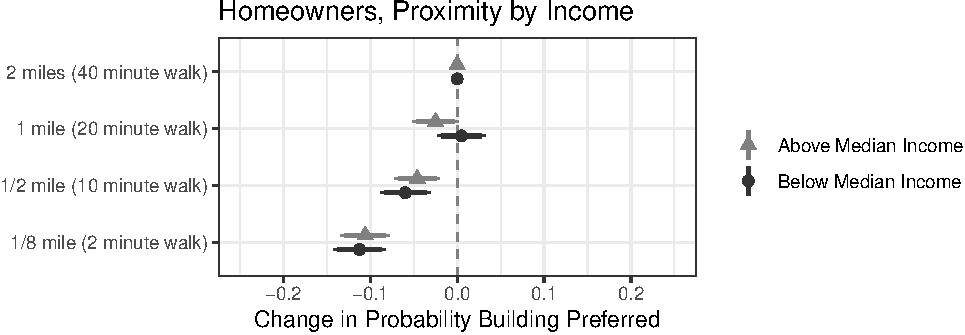
\includegraphics{Zheng-Ruth-Renters-Paper_files/figure-latex/Figure C.1 print-1.pdf}

\hypertarget{figure-c.2.-homeowner-spatial-sensitivity-by-ideology}{%
\subsubsection{Figure C.2. Homeowner Spatial Sensitivity by Ideology}\label{figure-c.2.-homeowner-spatial-sensitivity-by-ideology}}

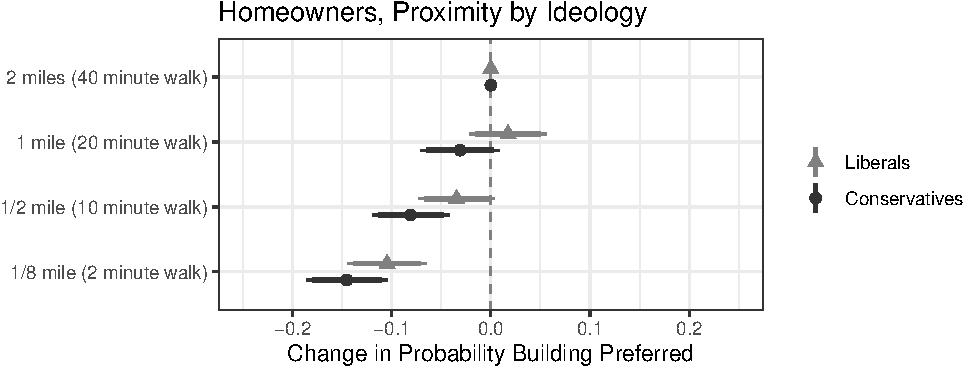
\includegraphics{Zheng-Ruth-Renters-Paper_files/figure-latex/Figure C2 print-1.pdf}

\hypertarget{figure-c.3.-effect-of-an-eighth-mile-away-compared-to-baseline-of-two-miles-away-for-each-level-of-affordability-by-homeownership-status}{%
\subsubsection{Figure C.3. Effect of an Eighth-Mile Away Compared to Baseline of Two Miles Away for Each Level of Affordability, by Homeownership Status}\label{figure-c.3.-effect-of-an-eighth-mile-away-compared-to-baseline-of-two-miles-away-for-each-level-of-affordability-by-homeownership-status}}

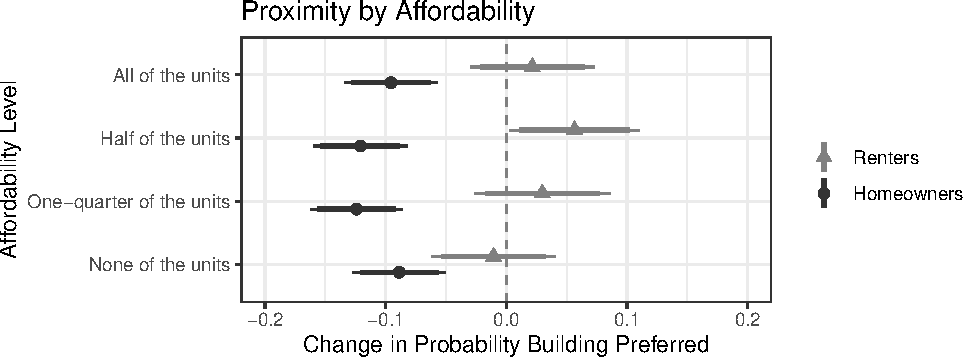
\includegraphics{Zheng-Ruth-Renters-Paper_files/figure-latex/Figure C.3 print-1.pdf}

\hypertarget{figure-c.4.-renter-spatial-sensitivity-toward-all-affordability-levels-by-citywide-average-rent}{%
\subsubsection{Figure C.4. Renter Spatial Sensitivity toward all Affordability Levels, by Citywide Average Rent}\label{figure-c.4.-renter-spatial-sensitivity-toward-all-affordability-levels-by-citywide-average-rent}}

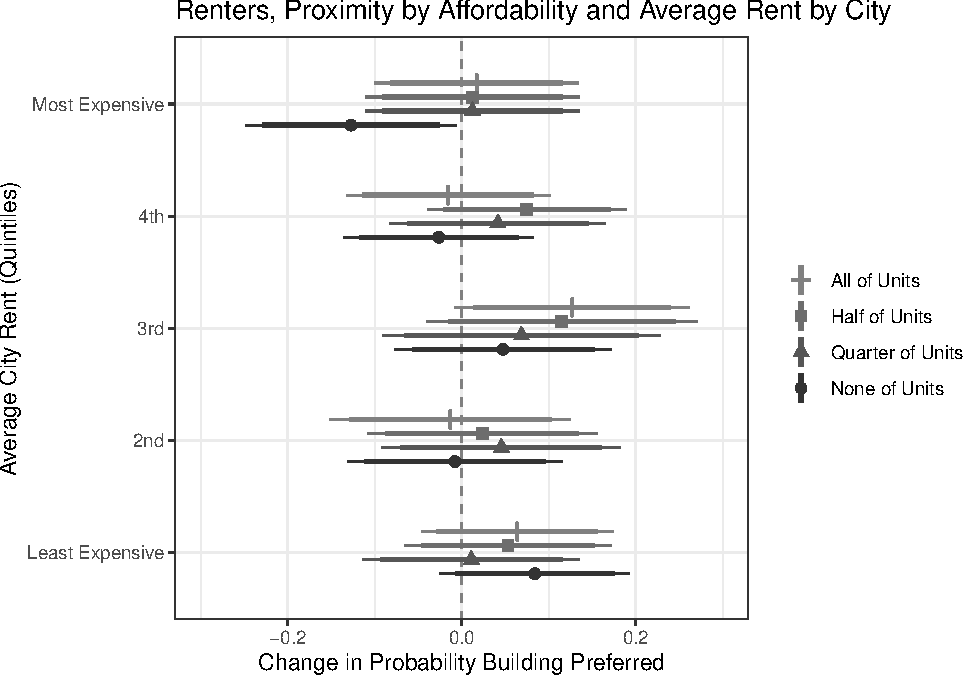
\includegraphics{Zheng-Ruth-Renters-Paper_files/figure-latex/Figure C.4 print-1.pdf}

\hypertarget{figure-c.5.-renter-spatial-sensitivity-toward-affordability-levels-by-zip-code-average-rent}{%
\subsubsection{Figure C.5. Renter Spatial Sensitivity toward Affordability Levels, by ZIP Code Average Rent}\label{figure-c.5.-renter-spatial-sensitivity-toward-affordability-levels-by-zip-code-average-rent}}

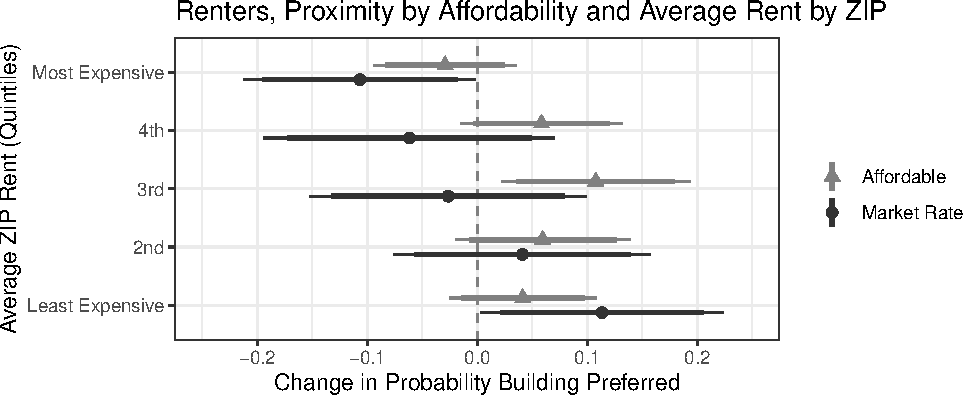
\includegraphics{Zheng-Ruth-Renters-Paper_files/figure-latex/Figure C.5 print-1.pdf}

\hypertarget{figure-c.6.-homeowner-spatial-sensitivity-to-all-affordability-levels-by-citywide-average-rent}{%
\subsubsection{Figure C.6. Homeowner Spatial Sensitivity to all Affordability Levels, by Citywide Average Rent}\label{figure-c.6.-homeowner-spatial-sensitivity-to-all-affordability-levels-by-citywide-average-rent}}

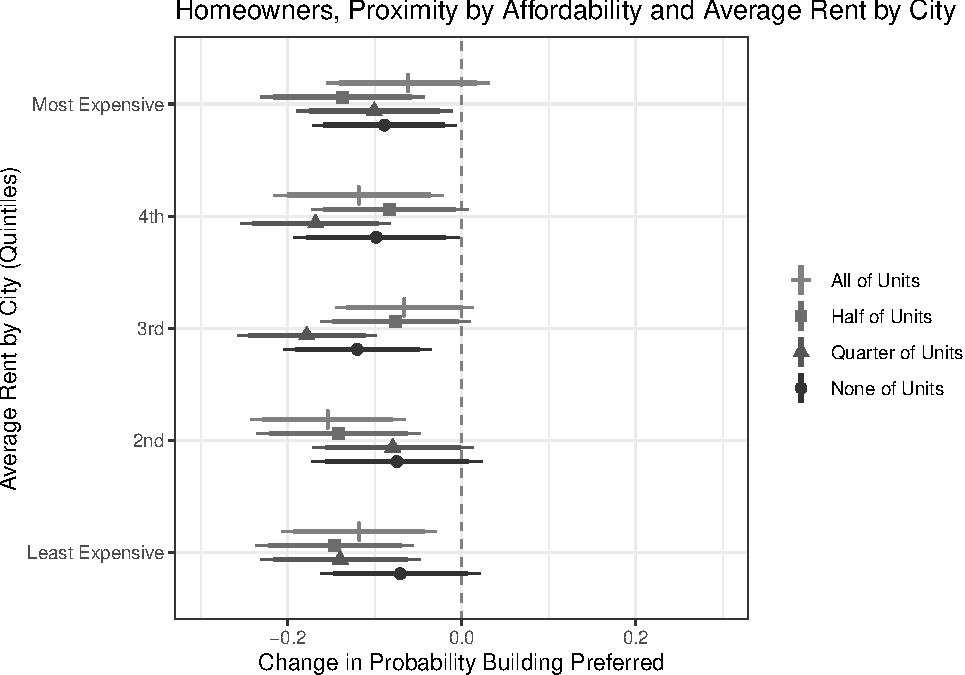
\includegraphics{Zheng-Ruth-Renters-Paper_files/figure-latex/Figure C.6 print-1.pdf}

\hypertarget{figure-c.7.-renter-spatial-sensitivity-toward-affordable-housing-by-price-anxiety.-note-lack-of-divergence-between-price-anxious-and-price-neutral-compared-to-preferences-toward-market-rate-housing-figure-7}{%
\subsubsection{Figure C.7. Renter Spatial Sensitivity toward Affordable Housing, by Price Anxiety. Note Lack of Divergence between ``Price Anxious'' and ``Price Neutral'' Compared to Preferences toward Market-Rate Housing (Figure 7)}\label{figure-c.7.-renter-spatial-sensitivity-toward-affordable-housing-by-price-anxiety.-note-lack-of-divergence-between-price-anxious-and-price-neutral-compared-to-preferences-toward-market-rate-housing-figure-7}}

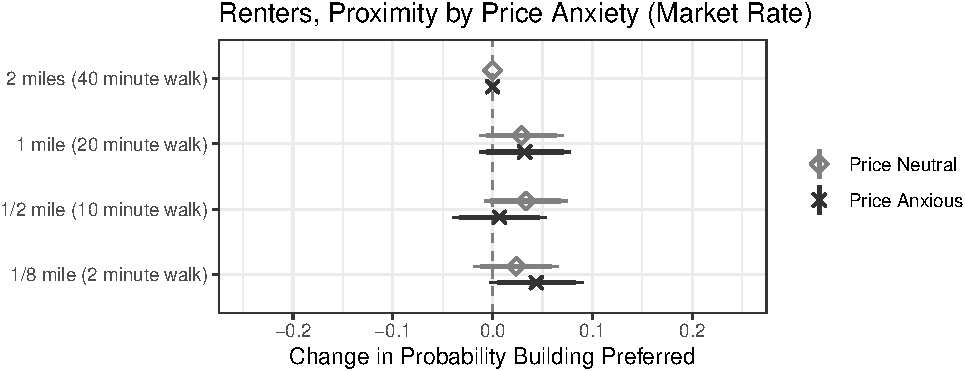
\includegraphics{Zheng-Ruth-Renters-Paper_files/figure-latex/Figure C.7 print-1.pdf}

\hypertarget{figure-c.8.-renter-support-for-a-10-increase-in-their-citytowns-housing-supply-grouped-into-quintiles-by-zip-code-average-rent}{%
\subsubsection{Figure C.8. Renter Support for a 10\% Increase in Their City/Town's Housing Supply, Grouped into Quintiles by ZIP Code Average Rent}\label{figure-c.8.-renter-support-for-a-10-increase-in-their-citytowns-housing-supply-grouped-into-quintiles-by-zip-code-average-rent}}

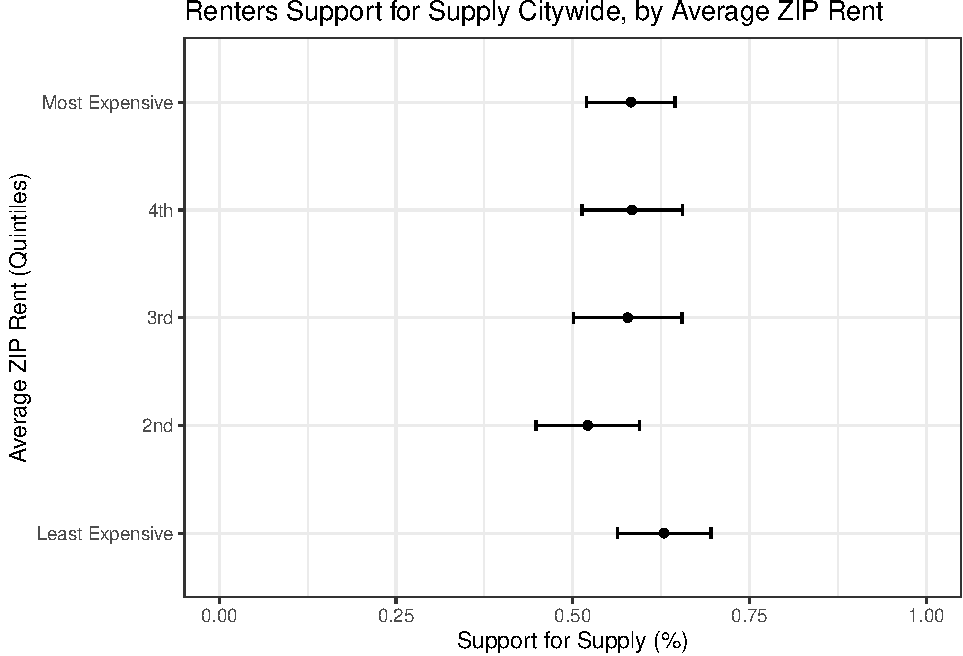
\includegraphics{Zheng-Ruth-Renters-Paper_files/figure-latex/Figure C.8 print-1.pdf}

\hypertarget{figure-c.9.-homeowner-support-for-a-10-increase-in-citytowns-housing-supply-by-citywide-average-rent}{%
\subsubsection{Figure C.9. Homeowner Support for a 10\% Increase in City/Town's Housing Supply, by Citywide Average Rent}\label{figure-c.9.-homeowner-support-for-a-10-increase-in-citytowns-housing-supply-by-citywide-average-rent}}

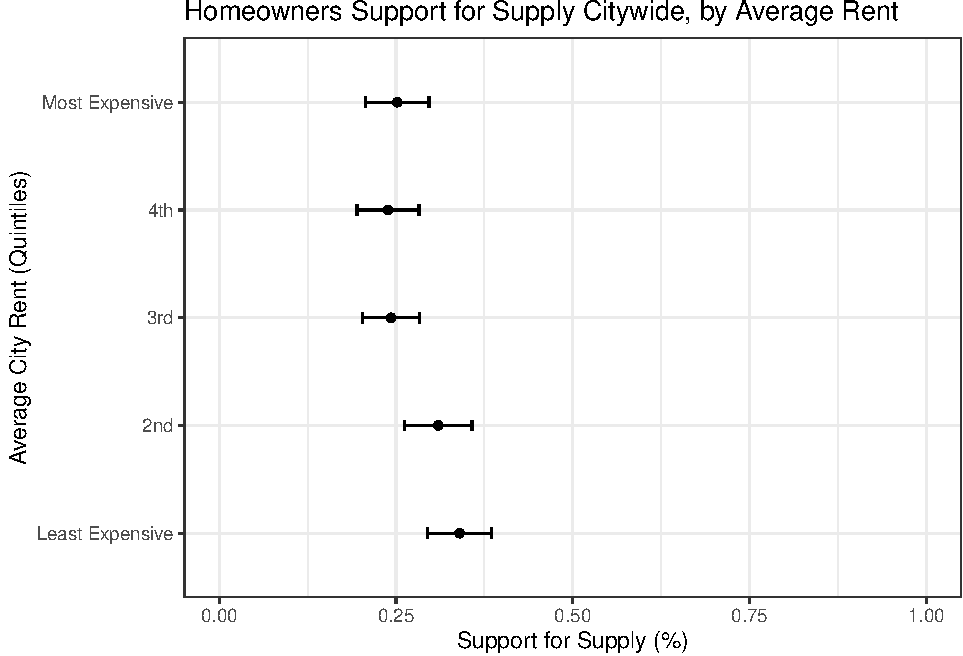
\includegraphics{Zheng-Ruth-Renters-Paper_files/figure-latex/Print Figure C.9-1.pdf}

\hypertarget{appendix}{%
\section{Appendix}\label{appendix}}

\begin{Shaded}
\begin{Highlighting}[]
\NormalTok{socpoc<-}\KeywordTok{read.csv}\NormalTok{(}\StringTok{"data/socpocAPSR.csv"}\NormalTok{, }\DataTypeTok{stringsAsFactors =}\NormalTok{ F)}

\CommentTok{#assign ownership groups}
\NormalTok{renters.socpoc<-}\KeywordTok{subset}\NormalTok{(socpoc, own}\OperatorTok{==}\DecValTok{0}\NormalTok{)}
\NormalTok{owners.socpoc<-}\KeywordTok{subset}\NormalTok{(socpoc, own}\OperatorTok{==}\DecValTok{1}\NormalTok{)}


\NormalTok{conjoint4<-}\KeywordTok{read.csv}\NormalTok{(}\StringTok{"data/conjointDataAPSR.csv"}\NormalTok{)}
\KeywordTok{table}\NormalTok{(conjoint4}\OperatorTok{$}\NormalTok{own)}
\CommentTok{#relevel}
\NormalTok{conjoint4}\OperatorTok{$}\NormalTok{distance <-}\StringTok{ }\KeywordTok{factor}\NormalTok{(conjoint4}\OperatorTok{$}\NormalTok{distance,}\DataTypeTok{levels=} \KeywordTok{c}\NormalTok{(}\StringTok{"2 miles (40 minute walk)"}\NormalTok{, }\StringTok{"1 mile (20 minute walk)"}\NormalTok{, }\StringTok{"1/2 mile (10 minute walk)"}\NormalTok{,}\StringTok{"1/8 mile (2 minute walk)"}\NormalTok{))}
\NormalTok{conjoint4}\OperatorTok{$}\NormalTok{community <-}\StringTok{ }\KeywordTok{factor}\NormalTok{(conjoint4}\OperatorTok{$}\NormalTok{community,}\DataTypeTok{levels=} \KeywordTok{c}\NormalTok{(}\StringTok{"No opinion"}\NormalTok{, }\StringTok{"Support the building"}\NormalTok{, }\StringTok{"Oppose the building"}\NormalTok{))}
\NormalTok{conjoint4}\OperatorTok{$}\NormalTok{affordable <-}\StringTok{ }\KeywordTok{factor}\NormalTok{(conjoint4}\OperatorTok{$}\NormalTok{affordable,}\DataTypeTok{levels=} \KeywordTok{c}\NormalTok{(}\StringTok{"None of the units"}\NormalTok{, }\StringTok{"One-quarter of the units"}\NormalTok{, }\StringTok{"Half of the units"}\NormalTok{, }\StringTok{"All of the units"}\NormalTok{))}
\NormalTok{conjoint4}\OperatorTok{$}\NormalTok{height <-}\StringTok{ }\KeywordTok{factor}\NormalTok{(conjoint4}\OperatorTok{$}\NormalTok{height,}\DataTypeTok{levels=} \KeywordTok{c}\NormalTok{(}\StringTok{"2 stories"}\NormalTok{, }\StringTok{"3 stories"}\NormalTok{, }\StringTok{"6 stories"}\NormalTok{, }\StringTok{"12 stories"}\NormalTok{))}
\NormalTok{conjoint4}\OperatorTok{$}\NormalTok{site <-}\StringTok{ }\KeywordTok{factor}\NormalTok{(conjoint4}\OperatorTok{$}\NormalTok{site, }\DataTypeTok{levels=}\KeywordTok{c}\NormalTok{(}\StringTok{"Empty building"}\NormalTok{,}\StringTok{"Parking lot"}\NormalTok{,}\StringTok{"Open field"}\NormalTok{,}\StringTok{"Historically-designated building"}\NormalTok{))}
\KeywordTok{names}\NormalTok{(conjoint4)}
\CommentTok{#reclassify items as factor}
\NormalTok{cols<-}\KeywordTok{c}\NormalTok{(}\StringTok{"own"}\NormalTok{, }\StringTok{"whitenh"}\NormalTok{, }\StringTok{"nearby"}\NormalTok{,}\StringTok{"conjoint_first"}\NormalTok{,}\StringTok{"rich"}\NormalTok{, }\StringTok{"luxury"}\NormalTok{)}

\NormalTok{conjoint4[cols] <-}\StringTok{ }\KeywordTok{data.frame}\NormalTok{(}\KeywordTok{apply}\NormalTok{(conjoint4[}\KeywordTok{c}\NormalTok{(cols)], }\DecValTok{2}\NormalTok{, as.factor))}

\CommentTok{# dummies}
\NormalTok{conjoint4}\OperatorTok{$}\NormalTok{liberal<-}\KeywordTok{as.factor}\NormalTok{(}\KeywordTok{ifelse}\NormalTok{(conjoint4}\OperatorTok{$}\NormalTok{ideology}\OperatorTok{>}\DecValTok{4}\NormalTok{,}\DecValTok{1}\NormalTok{,}\KeywordTok{ifelse}\NormalTok{(conjoint4}\OperatorTok{$}\NormalTok{ideology}\OperatorTok{<}\DecValTok{4}\NormalTok{,}\DecValTok{0}\NormalTok{, }\OtherTok{NA}\NormalTok{)))}
\NormalTok{conjoint4}\OperatorTok{$}\NormalTok{city_interest_low<-}\KeywordTok{as.factor}\NormalTok{(}\KeywordTok{ifelse}\NormalTok{(conjoint4}\OperatorTok{$}\NormalTok{city_interest}\OperatorTok{<}\DecValTok{0}\NormalTok{,}\DecValTok{1}\NormalTok{,}\DecValTok{0}\NormalTok{))}

\CommentTok{#define subgroups/dummies}
\NormalTok{renters.conjoint<-}\KeywordTok{subset}\NormalTok{(conjoint4, own}\OperatorTok{==}\DecValTok{0}\NormalTok{)}
\NormalTok{owners.conjoint<-}\KeywordTok{subset}\NormalTok{(conjoint4, own}\OperatorTok{==}\DecValTok{1}\NormalTok{)}

\CommentTok{#define affordability levels}
\NormalTok{renters_aff<-}\KeywordTok{subset}\NormalTok{(renters.conjoint, aff_housing}\OperatorTok{==}\DecValTok{1}\NormalTok{)}
\NormalTok{renters_lux<-}\KeywordTok{subset}\NormalTok{(renters.conjoint, aff_housing}\OperatorTok{==}\DecValTok{0}\NormalTok{)}

\NormalTok{owners_aff<-}\KeywordTok{subset}\NormalTok{(owners.conjoint, aff_housing}\OperatorTok{==}\DecValTok{1}\NormalTok{)}
\NormalTok{owners_lux<-}\KeywordTok{subset}\NormalTok{(owners.conjoint, aff_housing}\OperatorTok{==}\DecValTok{0}\NormalTok{)}


\CommentTok{# Read in Data}

\NormalTok{final<-}\KeywordTok{read.csv}\NormalTok{(}\StringTok{"data/sfDataAPSR.csv"}\NormalTok{, }\DataTypeTok{stringsAsFactors =}\NormalTok{ F)}

\NormalTok{owners.sf<-}\KeywordTok{subset}\NormalTok{(final, ownership_dummy}\OperatorTok{==}\DecValTok{1}\NormalTok{)}
\NormalTok{renters.sf<-}\KeywordTok{subset}\NormalTok{(final, ownership_dummy}\OperatorTok{==}\DecValTok{0}\NormalTok{)}

\CommentTok{# Experiment randomization}

\NormalTok{control<-}\KeywordTok{subset}\NormalTok{(final, version}\OperatorTok{==}\DecValTok{5} \OperatorTok{|}\StringTok{ }\NormalTok{version}\OperatorTok{==}\DecValTok{6}\NormalTok{)}
\NormalTok{control_owners<-}\KeywordTok{subset}\NormalTok{(control, ownership_dummy}\OperatorTok{==}\DecValTok{1}\NormalTok{)}
\NormalTok{control_renters<-}\KeywordTok{subset}\NormalTok{(control, ownership_dummy}\OperatorTok{==}\DecValTok{0}\NormalTok{)}

\NormalTok{control_owners_yes<-}\KeywordTok{subset}\NormalTok{(control_owners, ten_plan_dummy}\OperatorTok{==}\DecValTok{1}\NormalTok{)}
\NormalTok{control_owners_no<-}\KeywordTok{subset}\NormalTok{(control_owners, ten_plan_dummy}\OperatorTok{==}\DecValTok{0}\NormalTok{)}

\NormalTok{control_renters_yes<-}\KeywordTok{subset}\NormalTok{(control_renters, ten_plan_dummy}\OperatorTok{==}\DecValTok{1}\NormalTok{)}
\NormalTok{control_renters_no<-}\KeywordTok{subset}\NormalTok{(control_renters, ten_plan_dummy}\OperatorTok{==}\DecValTok{0}\NormalTok{)}


\CommentTok{# Extension Table A.3: Policy Proposals, SF}

\CommentTok{# Run Regressions}

\NormalTok{simple_control<-(}\KeywordTok{glm}\NormalTok{(ten_plan_dummy }\OperatorTok{~}\StringTok{ }\NormalTok{ownership_dummy, final, }\DataTypeTok{family =} \StringTok{"binomial"}\NormalTok{)); }\KeywordTok{summary}\NormalTok{(simple_control)}

\NormalTok{simple_control_se<-}\KeywordTok{sqrt}\NormalTok{(}\KeywordTok{diag}\NormalTok{(}\KeywordTok{vcovHC}\NormalTok{(simple_control, }\DataTypeTok{type=}\StringTok{"HC1"}\NormalTok{)))}

\NormalTok{full_control<-(}\KeywordTok{glm}\NormalTok{(ten_plan_dummy }\OperatorTok{~}\StringTok{ }\NormalTok{ownership_dummy  }\OperatorTok{+}\StringTok{  }\KeywordTok{scale}\NormalTok{(ideology_num) }\OperatorTok{+}\KeywordTok{scale}\NormalTok{(income_num) }\OperatorTok{+}\StringTok{ }\NormalTok{white_dummy  }\OperatorTok{+}\StringTok{ }\NormalTok{age}\OperatorTok{+}\StringTok{ }\NormalTok{gender_dummy , control, }\DataTypeTok{family =} \StringTok{"binomial"}\NormalTok{)); }\KeywordTok{summary}\NormalTok{(full_control)}
\NormalTok{full_control_se<-}\KeywordTok{sqrt}\NormalTok{(}\KeywordTok{diag}\NormalTok{(}\KeywordTok{vcovHC}\NormalTok{(full_control, }\DataTypeTok{type=}\StringTok{"HC1"}\NormalTok{)))}

\CommentTok{#Supplementary Data}
\KeywordTok{stargazer}\NormalTok{(simple_control, full_control, }\DataTypeTok{title=}\StringTok{"Ten Percent Supply Increase, San Francisco"}\NormalTok{,  }\DataTypeTok{label=}\StringTok{"ten_pct_dummy"}\NormalTok{, }
          \DataTypeTok{dep.var.labels=}\KeywordTok{c}\NormalTok{(}\StringTok{"Support Supply Increase"}\NormalTok{), }\DataTypeTok{dep.var.labels.include =}\NormalTok{ F, }\DataTypeTok{dev.var.caption=}\StringTok{""}\NormalTok{,}
          \DataTypeTok{column.labels=}\KeywordTok{c}\NormalTok{(}\StringTok{"Bivariate"}\NormalTok{, }\StringTok{"Full"}\NormalTok{),}
          \DataTypeTok{covariate.labels=}\KeywordTok{c}\NormalTok{(}\StringTok{"Homeownership"}\NormalTok{,}\StringTok{"Ideology"}\NormalTok{,}\StringTok{"Income, Log"}\NormalTok{,}\StringTok{"White, Non-Hispanic"}\NormalTok{,}\StringTok{"Age"}\NormalTok{,}\StringTok{"Male"}\NormalTok{),}
          \DataTypeTok{omit.stat=}\KeywordTok{c}\NormalTok{(}\StringTok{"ser"}\NormalTok{,}\StringTok{"f"}\NormalTok{), }\DataTypeTok{digits=}\DecValTok{2}\NormalTok{, }\DataTypeTok{align=}\NormalTok{T,}
          \DataTypeTok{initial.zero =}\NormalTok{ F, }\DataTypeTok{font.size=}\StringTok{"small"}\NormalTok{, }\DataTypeTok{star.cutoffs =} \OtherTok{NA}\NormalTok{, }\DataTypeTok{omit.table.layout=}\StringTok{"n"}\NormalTok{,}
          \DataTypeTok{se=}\KeywordTok{list}\NormalTok{(simple_control_se, full_control_se), }\DataTypeTok{no.space=}\NormalTok{T, }\DataTypeTok{omit=}\KeywordTok{c}\NormalTok{(}\StringTok{"name"}\NormalTok{))}


\CommentTok{#model ban}
\NormalTok{simple_prop_i_ban<-(}\KeywordTok{glm}\NormalTok{(prop_i_ban_dummy }\OperatorTok{~}\StringTok{ }\NormalTok{ownership_dummy  , final, }\DataTypeTok{family =} \StringTok{"binomial"}\NormalTok{)); }\KeywordTok{summary}\NormalTok{(simple_prop_i_ban)}
\NormalTok{simple_prop_i_ban_se<-}\KeywordTok{sqrt}\NormalTok{(}\KeywordTok{diag}\NormalTok{(}\KeywordTok{vcovHC}\NormalTok{(simple_prop_i_ban, }\DataTypeTok{type=}\StringTok{"HC1"}\NormalTok{)))}

\NormalTok{full_prop_i_ban<-(}\KeywordTok{glm}\NormalTok{(prop_i_ban_dummy }\OperatorTok{~}\StringTok{ }\NormalTok{ownership_dummy  }\OperatorTok{+}\StringTok{  }\KeywordTok{scale}\NormalTok{(ideology_num) }\OperatorTok{+}\KeywordTok{scale}\NormalTok{(income_num) }\OperatorTok{+}\StringTok{ }\NormalTok{white_dummy  }\OperatorTok{+}\StringTok{ }\NormalTok{age}\OperatorTok{+}\StringTok{ }\NormalTok{gender_dummy , final, }\DataTypeTok{family =} \StringTok{"binomial"}\NormalTok{)); }\KeywordTok{summary}\NormalTok{(full_prop_i_ban)}
\NormalTok{full_prop_i_ban_se<-}\KeywordTok{sqrt}\NormalTok{(}\KeywordTok{diag}\NormalTok{(}\KeywordTok{vcovHC}\NormalTok{(full_prop_i_ban, }\DataTypeTok{type=}\StringTok{"HC1"}\NormalTok{)))}

\CommentTok{#Table. Ban support}
\KeywordTok{stargazer}\NormalTok{(simple_prop_i_ban, full_prop_i_ban, }\DataTypeTok{title=}\StringTok{"Neighborhood Ban, San Francisco"}\NormalTok{,  }\DataTypeTok{label=}\StringTok{"prop_i_ban_dummy"}\NormalTok{,}
          \DataTypeTok{dep.var.labels=}\KeywordTok{c}\NormalTok{(}\StringTok{"Support Supply Increase"}\NormalTok{), }\DataTypeTok{dep.var.labels.include =}\NormalTok{ F, }\DataTypeTok{dev.var.caption=}\StringTok{""}\NormalTok{,}
          \DataTypeTok{column.labels=}\KeywordTok{c}\NormalTok{(}\StringTok{"Bivariate"}\NormalTok{, }\StringTok{"Full"}\NormalTok{),}
          \DataTypeTok{covariate.labels=}\KeywordTok{c}\NormalTok{(}\StringTok{"Homeownership"}\NormalTok{,}\StringTok{"Ideology"}\NormalTok{,}\StringTok{"Income, Log"}\NormalTok{,}\StringTok{"White, Non-Hispanic"}\NormalTok{,}\StringTok{"Age"}\NormalTok{,}\StringTok{"Male"}\NormalTok{),}
          \DataTypeTok{omit.stat=}\KeywordTok{c}\NormalTok{(}\StringTok{"ser"}\NormalTok{,}\StringTok{"f"}\NormalTok{), }\DataTypeTok{digits=}\DecValTok{2}\NormalTok{, }\DataTypeTok{align=}\NormalTok{T,}
          \DataTypeTok{initial.zero =}\NormalTok{ F, }\DataTypeTok{font.size=}\StringTok{"small"}\NormalTok{, }\DataTypeTok{star.cutoffs =} \OtherTok{NA}\NormalTok{, }\DataTypeTok{omit.table.layout=}\StringTok{"n"}\NormalTok{,}
          \DataTypeTok{se=}\KeywordTok{list}\NormalTok{(simple_prop_i_ban_se, full_prop_i_ban_se), }\DataTypeTok{no.space=}\NormalTok{T, }\DataTypeTok{omit=}\KeywordTok{c}\NormalTok{(}\StringTok{"name"}\NormalTok{))}

\CommentTok{# Table. Combine these two tables}

\KeywordTok{stargazer}\NormalTok{(simple_control, full_control, simple_prop_i_ban, full_prop_i_ban, }\DataTypeTok{title=}\StringTok{"Policy Proposals, San Francisco Sample"}\NormalTok{,  }\DataTypeTok{label=}\StringTok{"sf_policies"}\NormalTok{,}
          \DataTypeTok{dep.var.labels.include =}\NormalTok{ F, }\DataTypeTok{dev.var.caption=}\StringTok{""}\NormalTok{,}
          \DataTypeTok{column.labels=}\KeywordTok{c}\NormalTok{(}\StringTok{"10 Pct Supply"}\NormalTok{, }\StringTok{"NIMBY Ban Proposal"}\NormalTok{ ), }\DataTypeTok{column.separate =} \KeywordTok{c}\NormalTok{(}\DecValTok{2}\NormalTok{, }\DecValTok{2}\NormalTok{),}
          \DataTypeTok{covariate.labels=}\KeywordTok{c}\NormalTok{(}\StringTok{"Homeownership"}\NormalTok{,}\StringTok{"Ideology"}\NormalTok{,}\StringTok{"Income, Log"}\NormalTok{,}\StringTok{"White, Non-Hispanic"}\NormalTok{,}\StringTok{"Age"}\NormalTok{,}\StringTok{"Male"}\NormalTok{),}
          \DataTypeTok{omit.stat=}\KeywordTok{c}\NormalTok{(}\StringTok{"ser"}\NormalTok{,}\StringTok{"f"}\NormalTok{), }\DataTypeTok{digits=}\DecValTok{2}\NormalTok{, }\DataTypeTok{align=}\NormalTok{T, }\DataTypeTok{type=}\StringTok{"latex"}\NormalTok{,}
          \DataTypeTok{initial.zero =}\NormalTok{ F, }\DataTypeTok{font.size=}\StringTok{"small"}\NormalTok{, }\DataTypeTok{star.cutoffs =} \OtherTok{NA}\NormalTok{, }\DataTypeTok{omit.table.layout=}\StringTok{"n"}\NormalTok{,}
          \DataTypeTok{se=}\KeywordTok{list}\NormalTok{(simple_control_se, full_control_se, simple_prop_i_ban_se, full_prop_i_ban_se), }\DataTypeTok{no.space=}\NormalTok{T, }\DataTypeTok{table.placement =} \StringTok{"H"}\NormalTok{ )}


\CommentTok{# Extension Table B.2 Support for 10% Supply Increase}

\CommentTok{# Run Regressionss}

\CommentTok{# Bivariate}

\NormalTok{supply_simple<-(}\KeywordTok{glm}\NormalTok{(supply_dummy }\OperatorTok{~}\StringTok{ }\NormalTok{own, socpoc, }\DataTypeTok{family =} \StringTok{"binomial"}\NormalTok{))}
\NormalTok{supply_simple_se<-}\KeywordTok{sqrt}\NormalTok{(}\KeywordTok{diag}\NormalTok{(}\KeywordTok{vcovHC}\NormalTok{(supply_simple, }\DataTypeTok{type=}\StringTok{"HC1"}\NormalTok{)))}

\CommentTok{# Full}

\NormalTok{supply_full<-(}\KeywordTok{glm}\NormalTok{(supply_dummy }\OperatorTok{~}\StringTok{ }\NormalTok{own }\OperatorTok{+}\KeywordTok{scale}\NormalTok{(ideology)}\OperatorTok{+}\KeywordTok{scale}\NormalTok{(}\KeywordTok{log}\NormalTok{(income)) }\OperatorTok{+}\StringTok{ }\NormalTok{whitenh  }\OperatorTok{+}\NormalTok{age }\OperatorTok{+}\StringTok{ }\NormalTok{male, }\KeywordTok{subset}\NormalTok{(socpoc), }\DataTypeTok{family =} \StringTok{"binomial"}\NormalTok{))}
\NormalTok{supply_full_se<-}\KeywordTok{sqrt}\NormalTok{(}\KeywordTok{diag}\NormalTok{(}\KeywordTok{vcovHC}\NormalTok{(supply_full, }\DataTypeTok{type=}\StringTok{"HC1"}\NormalTok{)))}

\CommentTok{# Full w/ fixed effects}

\NormalTok{supply_full_fe<-(}\KeywordTok{glm}\NormalTok{(supply_dummy }\OperatorTok{~}\StringTok{  }\NormalTok{own }\OperatorTok{+}\KeywordTok{scale}\NormalTok{(ideology)}\OperatorTok{+}\StringTok{ }\KeywordTok{scale}\NormalTok{(}\KeywordTok{log}\NormalTok{(income))}\OperatorTok{+}\StringTok{ }\NormalTok{whitenh  }\OperatorTok{+}\StringTok{ }\NormalTok{age }\OperatorTok{+}\StringTok{ }\NormalTok{male }\OperatorTok{+}\KeywordTok{factor}\NormalTok{(name), socpoc, }\DataTypeTok{family =} \StringTok{"binomial"}\NormalTok{))}
\NormalTok{supply_full_fe_se<-}\KeywordTok{sqrt}\NormalTok{(}\KeywordTok{diag}\NormalTok{(}\KeywordTok{vcovHC}\NormalTok{(supply_full_fe, }\DataTypeTok{type=}\StringTok{"HC1"}\NormalTok{)))}

\CommentTok{# Create Regression Table}

\KeywordTok{stargazer}\NormalTok{(supply_simple,  supply_full , supply_full_fe, }\DataTypeTok{title=}\StringTok{"Support for 10 Percent Supply Increase"}\NormalTok{, }\DataTypeTok{label=}\StringTok{"supply_7"}\NormalTok{,}
          \DataTypeTok{dep.var.labels=}\KeywordTok{c}\NormalTok{(}\StringTok{"Support Supply Increase"}\NormalTok{),}\DataTypeTok{dep.var.labels.include =}\NormalTok{ F, }\DataTypeTok{dep.var.caption =} \StringTok{""}\NormalTok{,}
          \DataTypeTok{column.labels=}\KeywordTok{c}\NormalTok{(}\StringTok{"Bivariate"}\NormalTok{,}\StringTok{"Full"}\NormalTok{,}\StringTok{"Full with Fixed Effects"}\NormalTok{),}
          \DataTypeTok{covariate.labels=}\KeywordTok{c}\NormalTok{(}\StringTok{"Homeownership"}\NormalTok{,}\StringTok{"Ideology"}\NormalTok{,}\StringTok{"Income, Log"}\NormalTok{,}\StringTok{"White, Non-Hispanic"}\NormalTok{,}\StringTok{"Age"}\NormalTok{,}\StringTok{"Male"}\NormalTok{),}
          \DataTypeTok{omit.stat =} \KeywordTok{c}\NormalTok{(}\StringTok{"ser"}\NormalTok{, }\StringTok{"f"}\NormalTok{), }\DataTypeTok{digits=}\DecValTok{2}\NormalTok{, }\DataTypeTok{align=}\NormalTok{T, }\DataTypeTok{type=}\StringTok{"latex"}\NormalTok{,}
          \DataTypeTok{initial.zero =}\NormalTok{ F,  }\DataTypeTok{font.size =} \StringTok{"small"}\NormalTok{, }\DataTypeTok{star.cutoffs =} \OtherTok{NA}\NormalTok{, }\DataTypeTok{omit.table.layout =} \StringTok{"n"}\NormalTok{,}
          \DataTypeTok{se=}\KeywordTok{list}\NormalTok{(supply_simple_se, supply_full_se, supply_full_fe_se), }\DataTypeTok{no.space=}\NormalTok{T,}\DataTypeTok{omit=}\KeywordTok{c}\NormalTok{(}\StringTok{"name"}\NormalTok{), }\DataTypeTok{table.placement =} \StringTok{"H"}\NormalTok{ )}


\CommentTok{# Extension Table B.3. Support for 10 Percent Supply Increase - 7 Point Scale }

\CommentTok{# Load MASS packages}

\KeywordTok{library}\NormalTok{(MASS)}

\CommentTok{# Factor the response variable}

\NormalTok{socpoc}\OperatorTok{$}\NormalTok{city_supply1 =}\StringTok{ }\KeywordTok{as.factor}\NormalTok{(socpoc}\OperatorTok{$}\NormalTok{city_supply)}

\CommentTok{# Run Regressions}

\CommentTok{# Bivariate}

\NormalTok{supply_}\DecValTok{7}\NormalTok{_simple<-(}\KeywordTok{polr}\NormalTok{(city_supply1 }\OperatorTok{~}\StringTok{ }\NormalTok{own, socpoc))}
\NormalTok{supply_}\DecValTok{7}\NormalTok{_simple_se<-}\KeywordTok{sqrt}\NormalTok{(}\KeywordTok{diag}\NormalTok{(}\KeywordTok{vcov}\NormalTok{(supply_}\DecValTok{7}\NormalTok{_simple, }\DataTypeTok{type=}\StringTok{"HC1"}\NormalTok{)))}

\CommentTok{# Full}

\NormalTok{supply_}\DecValTok{7}\NormalTok{_full<-(}\KeywordTok{polr}\NormalTok{(city_supply1 }\OperatorTok{~}\StringTok{ }\NormalTok{own }\OperatorTok{+}\KeywordTok{scale}\NormalTok{(ideology)}\OperatorTok{+}\KeywordTok{scale}\NormalTok{(}\KeywordTok{log}\NormalTok{(income)) }\OperatorTok{+}\StringTok{ }\NormalTok{whitenh  }\OperatorTok{+}\NormalTok{age }\OperatorTok{+}\StringTok{ }\NormalTok{male, }\KeywordTok{subset}\NormalTok{(socpoc)))}
\NormalTok{supply_}\DecValTok{7}\NormalTok{_full_se<-}\KeywordTok{sqrt}\NormalTok{(}\KeywordTok{diag}\NormalTok{(}\KeywordTok{vcov}\NormalTok{(supply_}\DecValTok{7}\NormalTok{_full, }\DataTypeTok{type=}\StringTok{"HC1"}\NormalTok{)))}

\CommentTok{# Full w/ fixed effects}

\NormalTok{supply_}\DecValTok{7}\NormalTok{_full_fe<-(}\KeywordTok{polr}\NormalTok{(city_supply1 }\OperatorTok{~}\StringTok{  }\NormalTok{own }\OperatorTok{+}\KeywordTok{scale}\NormalTok{(ideology)}\OperatorTok{+}\StringTok{ }\KeywordTok{scale}\NormalTok{(}\KeywordTok{log}\NormalTok{(income))}\OperatorTok{+}\StringTok{ }\NormalTok{whitenh  }\OperatorTok{+}\StringTok{ }\NormalTok{age }\OperatorTok{+}\StringTok{ }\NormalTok{male }\OperatorTok{+}\KeywordTok{factor}\NormalTok{(name), socpoc))}
\NormalTok{supply_}\DecValTok{7}\NormalTok{_full_fe_se<-}\KeywordTok{sqrt}\NormalTok{(}\KeywordTok{diag}\NormalTok{(}\KeywordTok{vcov}\NormalTok{(supply_}\DecValTok{7}\NormalTok{_full_fe, }\DataTypeTok{type=}\StringTok{"HC1"}\NormalTok{)))}

\CommentTok{# Create Table}

\KeywordTok{stargazer}\NormalTok{(supply_}\DecValTok{7}\NormalTok{_simple,  supply_}\DecValTok{7}\NormalTok{_full , supply_}\DecValTok{7}\NormalTok{_full_fe, }\DataTypeTok{title=}\StringTok{"Support for 10 Percent Supply Increase - 7 Point Scale"}\NormalTok{, }\DataTypeTok{label=}\StringTok{"supply_7"}\NormalTok{,}
          \DataTypeTok{dep.var.labels=}\KeywordTok{c}\NormalTok{(}\StringTok{"Support Supply Increase"}\NormalTok{),}\DataTypeTok{dep.var.labels.include =}\NormalTok{ F, }\DataTypeTok{dep.var.caption =} \StringTok{""}\NormalTok{,}
          \DataTypeTok{column.labels=}\KeywordTok{c}\NormalTok{(}\StringTok{"Bivariate"}\NormalTok{,}\StringTok{"Full"}\NormalTok{,}\StringTok{"Full with Fixed Effects"}\NormalTok{),}
          \DataTypeTok{covariate.labels=}\KeywordTok{c}\NormalTok{(}\StringTok{"Homeownership"}\NormalTok{,}\StringTok{"Ideology"}\NormalTok{,}\StringTok{"Income, Log"}\NormalTok{,}\StringTok{"White, Non-Hispanic"}\NormalTok{,}\StringTok{"Age"}\NormalTok{,}\StringTok{"Male"}\NormalTok{),}
          \DataTypeTok{omit.stat =} \KeywordTok{c}\NormalTok{(}\StringTok{"ser"}\NormalTok{, }\StringTok{"f"}\NormalTok{), }\DataTypeTok{digits=}\DecValTok{2}\NormalTok{, }\DataTypeTok{align=}\NormalTok{T, }\DataTypeTok{type=}\StringTok{"latex"}\NormalTok{,}
          \DataTypeTok{initial.zero =}\NormalTok{ F,  }\DataTypeTok{font.size =} \StringTok{"small"}\NormalTok{, }\DataTypeTok{star.cutoffs =} \OtherTok{NA}\NormalTok{, }\DataTypeTok{omit.table.layout =} \StringTok{"n"}\NormalTok{,}
          \DataTypeTok{se=}\KeywordTok{list}\NormalTok{(supply_}\DecValTok{7}\NormalTok{_simple_se, supply_}\DecValTok{7}\NormalTok{_full_se, supply_}\DecValTok{7}\NormalTok{_full_fe_se), }\DataTypeTok{no.space=}\NormalTok{T,}\DataTypeTok{omit=}\KeywordTok{c}\NormalTok{(}\StringTok{"name"}\NormalTok{), }\DataTypeTok{table.placement =} \StringTok{"H"}\NormalTok{ )}


\CommentTok{# Extension Table B.4. Support for Neighborhood Ban ####}

\CommentTok{# bivariate}
\NormalTok{ban_simple<-(}\KeywordTok{glm}\NormalTok{(ban_dummy }\OperatorTok{~}\StringTok{ }\NormalTok{own, socpoc, }\DataTypeTok{family =} \StringTok{"binomial"}\NormalTok{))}
\NormalTok{ban_simple_se<-}\KeywordTok{sqrt}\NormalTok{(}\KeywordTok{diag}\NormalTok{(}\KeywordTok{vcovHC}\NormalTok{(ban_simple, }\DataTypeTok{type=}\StringTok{"HC1"}\NormalTok{)))}

\CommentTok{# full}

\NormalTok{ban_full<-(}\KeywordTok{glm}\NormalTok{(ban_dummy }\OperatorTok{~}\StringTok{ }\NormalTok{own }\OperatorTok{+}\KeywordTok{scale}\NormalTok{(ideology)}\OperatorTok{+}\KeywordTok{scale}\NormalTok{(}\KeywordTok{log}\NormalTok{(income)) }\OperatorTok{+}\StringTok{ }\NormalTok{whitenh  }\OperatorTok{+}\NormalTok{age }\OperatorTok{+}\StringTok{ }\NormalTok{male, socpoc, }\DataTypeTok{family =} \StringTok{"binomial"}\NormalTok{))}
\NormalTok{ban_full_se<-}\KeywordTok{sqrt}\NormalTok{(}\KeywordTok{diag}\NormalTok{(}\KeywordTok{vcovHC}\NormalTok{(ban_full, }\DataTypeTok{type=}\StringTok{"HC1"}\NormalTok{)))}

\CommentTok{#full w/ fixed effects}
\NormalTok{ban_full_fe<-(}\KeywordTok{glm}\NormalTok{(ban_dummy }\OperatorTok{~}\StringTok{  }\NormalTok{own }\OperatorTok{+}\KeywordTok{scale}\NormalTok{(ideology)}\OperatorTok{+}\StringTok{ }\KeywordTok{scale}\NormalTok{(}\KeywordTok{log}\NormalTok{(income))}\OperatorTok{+}\StringTok{ }\NormalTok{whitenh  }\OperatorTok{+}\StringTok{ }\NormalTok{age }\OperatorTok{+}\StringTok{ }\NormalTok{male }\OperatorTok{+}\KeywordTok{factor}\NormalTok{(name), socpoc, }\DataTypeTok{family =} \StringTok{"binomial"}\NormalTok{))}
\NormalTok{ban_full_fe_se<-}\KeywordTok{sqrt}\NormalTok{(}\KeywordTok{diag}\NormalTok{(}\KeywordTok{vcovHC}\NormalTok{(ban_full_fe, }\DataTypeTok{type=}\StringTok{"HC1"}\NormalTok{)))}

\CommentTok{# Table}
\KeywordTok{stargazer}\NormalTok{(ban_simple,  ban_full , ban_full_fe, }\DataTypeTok{title=}\StringTok{"Support for Ban on Neighborhood Development"}\NormalTok{, }\DataTypeTok{label=}\StringTok{"ban_dummy"}\NormalTok{,}
          \DataTypeTok{dep.var.labels=}\KeywordTok{c}\NormalTok{(}\StringTok{"Support NIMBY Ban"}\NormalTok{),}\DataTypeTok{dep.var.labels.include =}\NormalTok{ F, }\DataTypeTok{dep.var.caption =} \StringTok{""}\NormalTok{,}
          \DataTypeTok{column.labels=}\KeywordTok{c}\NormalTok{(}\StringTok{"Bivariate"}\NormalTok{,}\StringTok{"Full"}\NormalTok{,}\StringTok{"Full with Fixed Effects"}\NormalTok{),}
          \DataTypeTok{covariate.labels=}\KeywordTok{c}\NormalTok{(}\StringTok{"Homeownership"}\NormalTok{,}\StringTok{"Ideology"}\NormalTok{,}\StringTok{"Income, Log"}\NormalTok{,}\StringTok{"White, Non-Hispanic"}\NormalTok{,}\StringTok{"Age"}\NormalTok{,}\StringTok{"Male"}\NormalTok{),}
          \DataTypeTok{omit.stat =} \KeywordTok{c}\NormalTok{(}\StringTok{"ser"}\NormalTok{, }\StringTok{"f"}\NormalTok{), }\DataTypeTok{digits=}\DecValTok{2}\NormalTok{, }\DataTypeTok{align=}\NormalTok{T, }\DataTypeTok{type=}\StringTok{"latex"}\NormalTok{,}
          \DataTypeTok{initial.zero =}\NormalTok{ F,  }\DataTypeTok{font.size =} \StringTok{"small"}\NormalTok{,}\DataTypeTok{star.cutoffs =} \OtherTok{NA}\NormalTok{, }\DataTypeTok{omit.table.layout =} \StringTok{"n"}\NormalTok{,}
          \DataTypeTok{se=}\KeywordTok{list}\NormalTok{(ban_simple_se, ban_full_se, ban_full_fe_se), }\DataTypeTok{no.space=}\NormalTok{T, }\DataTypeTok{omit=}\KeywordTok{c}\NormalTok{(}\StringTok{"name"}\NormalTok{), }\DataTypeTok{table.placement =} \StringTok{"H"}\NormalTok{ )}


\CommentTok{# Extension Table B.5. Support for Neighborhood Ban 7 point scale ####}

\CommentTok{# Factor the response variable}

\NormalTok{socpoc}\OperatorTok{$}\NormalTok{neighborhood_ban1 =}\StringTok{ }\KeywordTok{as.factor}\NormalTok{(socpoc}\OperatorTok{$}\NormalTok{neighborhood_ban)}

\CommentTok{# Run Regressions}

\CommentTok{#simple}

\NormalTok{ban_simple<-(}\KeywordTok{polr}\NormalTok{(neighborhood_ban1 }\OperatorTok{~}\StringTok{ }\NormalTok{own, socpoc))}
\NormalTok{ban_simple_se<-}\KeywordTok{sqrt}\NormalTok{(}\KeywordTok{diag}\NormalTok{(}\KeywordTok{vcov}\NormalTok{(ban_simple, }\DataTypeTok{type=}\StringTok{"HC1"}\NormalTok{)))}

\CommentTok{# full}

\NormalTok{ban_full<-(}\KeywordTok{polr}\NormalTok{(neighborhood_ban1 }\OperatorTok{~}\StringTok{ }\NormalTok{own }\OperatorTok{+}\KeywordTok{scale}\NormalTok{(ideology)}\OperatorTok{+}\KeywordTok{scale}\NormalTok{(}\KeywordTok{log}\NormalTok{(income)) }\OperatorTok{+}\StringTok{ }\NormalTok{whitenh  }\OperatorTok{+}\NormalTok{age }\OperatorTok{+}\StringTok{ }\NormalTok{male, socpoc))}
\NormalTok{ban_full_se<-}\KeywordTok{sqrt}\NormalTok{(}\KeywordTok{diag}\NormalTok{(}\KeywordTok{vcov}\NormalTok{(ban_full, }\DataTypeTok{type=}\StringTok{"HC1"}\NormalTok{)))}

\CommentTok{#full w/ fixed effects}

\NormalTok{ban_full_fe<-(}\KeywordTok{polr}\NormalTok{(neighborhood_ban1 }\OperatorTok{~}\StringTok{  }\NormalTok{own }\OperatorTok{+}\KeywordTok{scale}\NormalTok{(ideology)}\OperatorTok{+}\StringTok{ }\KeywordTok{scale}\NormalTok{(}\KeywordTok{log}\NormalTok{(income))}\OperatorTok{+}\StringTok{ }\NormalTok{whitenh  }\OperatorTok{+}\StringTok{ }\NormalTok{age }\OperatorTok{+}\StringTok{ }\NormalTok{male }\OperatorTok{+}\KeywordTok{factor}\NormalTok{(name), socpoc))}
\NormalTok{ban_full_fe_se<-}\KeywordTok{sqrt}\NormalTok{(}\KeywordTok{diag}\NormalTok{(}\KeywordTok{vcov}\NormalTok{(ban_full_fe, }\DataTypeTok{type=}\StringTok{"HC1"}\NormalTok{)))}

\CommentTok{# Table}
\KeywordTok{stargazer}\NormalTok{(ban_simple,  ban_full , ban_full_fe, }\DataTypeTok{title=}\StringTok{"Support for Ban on Neighborhood Development - 7 Point Scale"}\NormalTok{, }\DataTypeTok{label=}\StringTok{"neighborhood_ban_7"}\NormalTok{,}
          \DataTypeTok{dep.var.labels=}\KeywordTok{c}\NormalTok{(}\StringTok{"Support NIMBY Ban"}\NormalTok{),}\DataTypeTok{dep.var.labels.include =}\NormalTok{ F, }\DataTypeTok{dep.var.caption =} \StringTok{""}\NormalTok{,}
          \DataTypeTok{column.labels=}\KeywordTok{c}\NormalTok{(}\StringTok{"Bivariate"}\NormalTok{,}\StringTok{"Full"}\NormalTok{,}\StringTok{"Full with Fixed Effects"}\NormalTok{),}
          \DataTypeTok{covariate.labels=}\KeywordTok{c}\NormalTok{(}\StringTok{"Homeownership"}\NormalTok{,}\StringTok{"Ideology"}\NormalTok{,}\StringTok{"Income, Log"}\NormalTok{,}\StringTok{"White, Non-Hispanic"}\NormalTok{,}\StringTok{"Age"}\NormalTok{,}\StringTok{"Male"}\NormalTok{),}
          \DataTypeTok{omit.stat =} \KeywordTok{c}\NormalTok{(}\StringTok{"ser"}\NormalTok{, }\StringTok{"f"}\NormalTok{), }\DataTypeTok{digits=}\DecValTok{2}\NormalTok{, }\DataTypeTok{align=}\NormalTok{T, }\DataTypeTok{type=}\StringTok{"latex"}\NormalTok{,}
          \DataTypeTok{initial.zero =}\NormalTok{ F,  }\DataTypeTok{font.size =} \StringTok{"small"}\NormalTok{,}\DataTypeTok{star.cutoffs =} \OtherTok{NA}\NormalTok{, }\DataTypeTok{omit.table.layout =} \StringTok{"n"}\NormalTok{,}
          \DataTypeTok{se=}\KeywordTok{list}\NormalTok{(ban_simple_se, ban_full_se, ban_full_fe_se), }\DataTypeTok{no.space=}\NormalTok{T, }\DataTypeTok{omit=}\KeywordTok{c}\NormalTok{(}\StringTok{"name"}\NormalTok{), }\DataTypeTok{table.placement =} \StringTok{"H"}\NormalTok{ )}

\CommentTok{# Replication results begin here}

\NormalTok{support<-}\KeywordTok{c}\NormalTok{(.}\DecValTok{37}\NormalTok{, }\FloatTok{.50}\NormalTok{, }\FloatTok{.52}\NormalTok{, }\FloatTok{.81}\NormalTok{)}
\NormalTok{Tenant<-}\KeywordTok{c}\NormalTok{(}\StringTok{"Homeowners"}\NormalTok{, }\StringTok{"Homeowners"}\NormalTok{, }\StringTok{"Renters"}\NormalTok{, }\StringTok{"Renters"}\NormalTok{)}
\NormalTok{supply<-}\KeywordTok{c}\NormalTok{(}\StringTok{"Pro-Supply"}\NormalTok{, }\StringTok{"Anti-Supply"}\NormalTok{,}\StringTok{"Pro-Supply"}\NormalTok{,}\StringTok{"Anti-Supply"}\NormalTok{)}
\NormalTok{supply<-}\KeywordTok{factor}\NormalTok{(supply, }\DataTypeTok{levels=}\KeywordTok{c}\NormalTok{(}\StringTok{"Pro-Supply"}\NormalTok{, }\StringTok{"Anti-Supply"}\NormalTok{))}

\NormalTok{ban_plot<-}\KeywordTok{data.frame}\NormalTok{(Tenant, support, supply)}

\NormalTok{exitpoll_ban<-}\KeywordTok{ggplot}\NormalTok{(}\DataTypeTok{data=}\NormalTok{ban_plot, }\KeywordTok{aes}\NormalTok{(}\DataTypeTok{x=}\NormalTok{Tenant, }\DataTypeTok{y=}\NormalTok{support, }\DataTypeTok{fill=}\NormalTok{Tenant))}\OperatorTok{+}
\StringTok{  }\KeywordTok{geom_bar}\NormalTok{(}\DataTypeTok{colour=}\StringTok{"black"}\NormalTok{,}\DataTypeTok{stat=}\StringTok{"identity"}\NormalTok{, }\DataTypeTok{position=}\KeywordTok{position_dodge}\NormalTok{()) }\OperatorTok{+}\StringTok{ }\KeywordTok{facet_wrap}\NormalTok{(}\OperatorTok{~}\NormalTok{supply) }\OperatorTok{+}
\StringTok{  }\KeywordTok{ylab}\NormalTok{(}\StringTok{"Support (Percent)"}\NormalTok{) }\OperatorTok{+}\StringTok{ }\KeywordTok{theme}\NormalTok{(}\DataTypeTok{legend.position=}\StringTok{"none"}\NormalTok{) }\OperatorTok{+}\KeywordTok{ggtitle}\NormalTok{( }\StringTok{"Support for Micro-scale Ban by Support for Macro-scale Supply"}\NormalTok{)}\OperatorTok{+}
\StringTok{  }\KeywordTok{theme_bw}\NormalTok{()}\OperatorTok{+}\KeywordTok{scale_fill_grey}\NormalTok{()}

\NormalTok{exitpoll_ban}


\CommentTok{# FIGURE 3. Homeowners, Proximity by Affordability ####}


\CommentTok{# Use AMCE to run regressions}

\NormalTok{owners_luxury_mod<-}\KeywordTok{amce}\NormalTok{(select }\OperatorTok{~}\StringTok{ }\NormalTok{distance  }\OperatorTok{+}\StringTok{ }\NormalTok{community }\OperatorTok{+}\StringTok{ }\NormalTok{height }\OperatorTok{+}\StringTok{ }\NormalTok{site }\OperatorTok{+}\StringTok{ }\NormalTok{tenant }\OperatorTok{+}\StringTok{ }\NormalTok{units,}
                        \DataTypeTok{data=}\NormalTok{ owners_lux , }\DataTypeTok{cluster=}\NormalTok{T,  }\DataTypeTok{respondent.id =} \StringTok{"CaseID"}\NormalTok{)}
\NormalTok{owners_affordable_mod<-}\KeywordTok{amce}\NormalTok{(select }\OperatorTok{~}\StringTok{ }\NormalTok{distance  }\OperatorTok{+}\StringTok{ }\NormalTok{community }\OperatorTok{+}\StringTok{ }\NormalTok{height }\OperatorTok{+}\StringTok{ }\NormalTok{site }\OperatorTok{+}\StringTok{ }\NormalTok{tenant }\OperatorTok{+}\StringTok{ }\NormalTok{units,}
                            \DataTypeTok{data=}\NormalTok{owners_aff, }\DataTypeTok{cluster=}\NormalTok{T,  }\DataTypeTok{respondent.id =} \StringTok{"CaseID"}\NormalTok{)}
\NormalTok{owners_luxury_mod_frame<-}\KeywordTok{data.frame}\NormalTok{(}\DataTypeTok{Variable=}\NormalTok{(}\KeywordTok{summary}\NormalTok{(owners_luxury_mod)}\OperatorTok{$}\NormalTok{amce)}\OperatorTok{$}\NormalTok{Level,}
                                    \DataTypeTok{Coefficient =}\NormalTok{ (}\KeywordTok{summary}\NormalTok{(owners_luxury_mod)}\OperatorTok{$}\NormalTok{amce)}\OperatorTok{$}\NormalTok{Estimate,}
                                    \DataTypeTok{SE=}\NormalTok{(}\KeywordTok{summary}\NormalTok{(owners_luxury_mod)}\OperatorTok{$}\NormalTok{amce)}\OperatorTok{$}\StringTok{'Std. Err'}\NormalTok{,}
                                    \DataTypeTok{modelName=}\StringTok{"Market Rate"}\NormalTok{)}
\NormalTok{owners_affordable_mod_frame<-}\KeywordTok{data.frame}\NormalTok{(}\DataTypeTok{Variable=}\NormalTok{(}\KeywordTok{summary}\NormalTok{(owners_affordable_mod)}\OperatorTok{$}\NormalTok{amce)}\OperatorTok{$}\NormalTok{Level,}
                                        \DataTypeTok{Coefficient =}\NormalTok{ (}\KeywordTok{summary}\NormalTok{(owners_affordable_mod)}\OperatorTok{$}\NormalTok{amce)}\OperatorTok{$}\NormalTok{Estimate,}
                                        \DataTypeTok{SE=}\NormalTok{(}\KeywordTok{summary}\NormalTok{(owners_affordable_mod)}\OperatorTok{$}\NormalTok{amce)}\OperatorTok{$}\StringTok{'Std. Err'}\NormalTok{,}
                                        \DataTypeTok{modelName=}\StringTok{"Affordable"}\NormalTok{)}
\NormalTok{ownersPriceFrame<-}\KeywordTok{data.frame}\NormalTok{(}\KeywordTok{rbind}\NormalTok{(owners_luxury_mod_frame, owners_affordable_mod_frame))}
\NormalTok{ownersPriceFrame<-}\KeywordTok{subset}\NormalTok{(ownersPriceFrame, Variable}\OperatorTok{==}\StringTok{"1/8 mile (2 minute walk)"}\OperatorTok{|}\NormalTok{Variable}\OperatorTok{==}\StringTok{"1/2 mile (10 minute walk)"}\OperatorTok{|}\NormalTok{Variable}\OperatorTok{==}\StringTok{"1 mile (20 minute walk)"}\NormalTok{)}
\NormalTok{ownersPriceFrameIntercepts<-}\KeywordTok{data.frame}\NormalTok{(}\DataTypeTok{Variable=}\KeywordTok{c}\NormalTok{(}\StringTok{"2 miles (40 minute walk)"}\NormalTok{, }\StringTok{"2 miles (40 minute walk)"}\NormalTok{) ,}\DataTypeTok{Coefficient=}\KeywordTok{c}\NormalTok{(}\DecValTok{0}\NormalTok{,}\DecValTok{0}\NormalTok{), }\DataTypeTok{SE=}\KeywordTok{c}\NormalTok{(}\DecValTok{0}\NormalTok{,}\DecValTok{0}\NormalTok{), }\DataTypeTok{modelName=}\KeywordTok{c}\NormalTok{(}\StringTok{"Market Rate"}\NormalTok{, }\StringTok{"Affordable"}\NormalTok{))}
\NormalTok{ownersPriceFrame<-}\KeywordTok{data.frame}\NormalTok{(}\KeywordTok{rbind}\NormalTok{(ownersPriceFrame,ownersPriceFrameIntercepts))}
\NormalTok{interval1<-}\KeywordTok{qnorm}\NormalTok{((}\DecValTok{1}\FloatTok{-.9}\NormalTok{)}\OperatorTok{/}\DecValTok{2}\NormalTok{)}
\NormalTok{interval2<-}\KeywordTok{qnorm}\NormalTok{((}\DecValTok{1}\FloatTok{-.95}\NormalTok{)}\OperatorTok{/}\DecValTok{2}\NormalTok{)}
\NormalTok{ownersPriceFrame}\OperatorTok{$}\NormalTok{Variable <-}\StringTok{ }\KeywordTok{factor}\NormalTok{(ownersPriceFrame}\OperatorTok{$}\NormalTok{Variable, }\DataTypeTok{levels =} \KeywordTok{c}\NormalTok{(}\StringTok{"1/8 mile (2 minute walk)"}\NormalTok{,}\StringTok{"1/2 mile (10 minute walk)"}\NormalTok{, }\StringTok{"1 mile (20 minute walk)"}\NormalTok{, }\StringTok{"2 miles (40 minute walk)"}\NormalTok{))}

\CommentTok{# Plot ggplot. }

\NormalTok{owners_price_nimby<-}\KeywordTok{ggplot}\NormalTok{(ownersPriceFrame, }\KeywordTok{aes}\NormalTok{(}\DataTypeTok{colour=}\NormalTok{modelName, }\DataTypeTok{shape=}\NormalTok{modelName))}\OperatorTok{+}\StringTok{ }\KeywordTok{scale_y_continuous}\NormalTok{(}\DataTypeTok{limits =} \KeywordTok{c}\NormalTok{(}\OperatorTok{-}\NormalTok{.}\DecValTok{20}\NormalTok{, }\FloatTok{.20}\NormalTok{))}
\NormalTok{owners_price_nimby<-owners_price_nimby}\OperatorTok{+}\KeywordTok{theme_bw}\NormalTok{()}\OperatorTok{+}\KeywordTok{scale_colour_grey}\NormalTok{(}\DataTypeTok{end=}\NormalTok{.}\DecValTok{5}\NormalTok{)}\OperatorTok{+}\KeywordTok{geom_hline}\NormalTok{(}\DataTypeTok{yintercept=}\DecValTok{0}\NormalTok{, }\DataTypeTok{colour=}\KeywordTok{gray}\NormalTok{(}\DecValTok{1}\OperatorTok{/}\DecValTok{2}\NormalTok{), }\DataTypeTok{lty=}\DecValTok{2}\NormalTok{)}
\NormalTok{owners_price_nimby<-owners_price_nimby}\OperatorTok{+}\KeywordTok{geom_linerange}\NormalTok{(}\KeywordTok{aes}\NormalTok{(}\DataTypeTok{x=}\NormalTok{Variable, }\DataTypeTok{ymin=}\NormalTok{Coefficient}\OperatorTok{-}\NormalTok{SE}\OperatorTok{*}\NormalTok{interval1, }
                                                          \DataTypeTok{ymax=}\NormalTok{Coefficient}\OperatorTok{+}\NormalTok{SE}\OperatorTok{*}\NormalTok{interval1), }\DataTypeTok{lwd=}\DecValTok{1}\NormalTok{, }\DataTypeTok{position=}\KeywordTok{position_dodge}\NormalTok{(}\DataTypeTok{width=}\DecValTok{1}\OperatorTok{/}\DecValTok{2}\NormalTok{))}
\NormalTok{owners_price_nimby<-owners_price_nimby}\OperatorTok{+}\KeywordTok{geom_pointrange}\NormalTok{(}\KeywordTok{aes}\NormalTok{(}\DataTypeTok{x=}\NormalTok{Variable, }\DataTypeTok{y=}\NormalTok{Coefficient, }\DataTypeTok{ymin=}\NormalTok{Coefficient}\OperatorTok{-}\NormalTok{SE}\OperatorTok{*}\NormalTok{interval2,}
                                                           \DataTypeTok{ymax=}\NormalTok{Coefficient}\OperatorTok{+}\NormalTok{SE}\OperatorTok{*}\NormalTok{interval2), }\DataTypeTok{lwd=}\DecValTok{1}\OperatorTok{/}\DecValTok{2}\NormalTok{,}
                                                       \DataTypeTok{position=}\KeywordTok{position_dodge}\NormalTok{(}\DataTypeTok{width=}\DecValTok{1}\OperatorTok{/}\DecValTok{2}\NormalTok{), }\DataTypeTok{fill=}\StringTok{"WHITE"}\NormalTok{)}
\NormalTok{owners_price_nimby<-owners_price_nimby}\OperatorTok{+}\KeywordTok{coord_flip}\NormalTok{()}\OperatorTok{+}\KeywordTok{labs}\NormalTok{(}\DataTypeTok{y=}\StringTok{"Change in Probability Building Preferred"}\NormalTok{)}
\NormalTok{owners_price_nimby<-owners_price_nimby}\OperatorTok{+}\KeywordTok{theme}\NormalTok{(}\DataTypeTok{legend.title=}\KeywordTok{element_blank}\NormalTok{(),}\DataTypeTok{axis.title.y=}\KeywordTok{element_blank}\NormalTok{())}\OperatorTok{+}\StringTok{ }\KeywordTok{theme}\NormalTok{(}\DataTypeTok{aspect.ratio =} \FloatTok{.5}\NormalTok{)}
\NormalTok{owners_price_nimby<-owners_price_nimby}\OperatorTok{+}\KeywordTok{theme}\NormalTok{(}\DataTypeTok{plot.margin=}\KeywordTok{unit}\NormalTok{(}\KeywordTok{c}\NormalTok{(}\DecValTok{0}\NormalTok{,}\DecValTok{0}\NormalTok{,}\DecValTok{0}\NormalTok{,}\DecValTok{0}\NormalTok{),}\StringTok{"mm"}\NormalTok{))}\OperatorTok{+}\KeywordTok{ggtitle}\NormalTok{(}\StringTok{"Homeowners, Proximity by Affordability"}\NormalTok{) }\OperatorTok{+}\StringTok{ }\KeywordTok{guides}\NormalTok{(}\DataTypeTok{colour=}\KeywordTok{guide_legend}\NormalTok{(}\DataTypeTok{reverse=}\NormalTok{T), }\DataTypeTok{shape=}\KeywordTok{guide_legend}\NormalTok{(}\DataTypeTok{reverse=}\NormalTok{T))}


\KeywordTok{print}\NormalTok{(owners_price_nimby)}


\CommentTok{# FIGURE 4. Renters, Proximity by Affordability ####}
\NormalTok{renters_luxury_mod<-}\KeywordTok{amce}\NormalTok{(select }\OperatorTok{~}\StringTok{ }\NormalTok{distance  }\OperatorTok{+}\StringTok{ }\NormalTok{community }\OperatorTok{+}\StringTok{ }\NormalTok{height }\OperatorTok{+}\StringTok{ }\NormalTok{site }\OperatorTok{+}\StringTok{ }\NormalTok{tenant }\OperatorTok{+}\StringTok{ }\NormalTok{units,}
                         \DataTypeTok{data=}\NormalTok{ renters_lux , }\DataTypeTok{cluster=}\NormalTok{T,  }\DataTypeTok{respondent.id =} \StringTok{"CaseID"}\NormalTok{)}
\NormalTok{renters_affordable_mod<-}\KeywordTok{amce}\NormalTok{(select }\OperatorTok{~}\StringTok{ }\NormalTok{distance  }\OperatorTok{+}\StringTok{ }\NormalTok{community }\OperatorTok{+}\StringTok{ }\NormalTok{height }\OperatorTok{+}\StringTok{ }\NormalTok{site }\OperatorTok{+}\StringTok{ }\NormalTok{tenant }\OperatorTok{+}\StringTok{ }\NormalTok{units,}
                             \DataTypeTok{data=}\NormalTok{renters_aff, }\DataTypeTok{cluster=}\NormalTok{T,  }\DataTypeTok{respondent.id =} \StringTok{"CaseID"}\NormalTok{)}
\NormalTok{renters_luxury_mod_frame<-}\KeywordTok{data.frame}\NormalTok{(}\DataTypeTok{Variable=}\NormalTok{(}\KeywordTok{summary}\NormalTok{(renters_luxury_mod)}\OperatorTok{$}\NormalTok{amce)}\OperatorTok{$}\NormalTok{Level,}
                                     \DataTypeTok{Coefficient =}\NormalTok{ (}\KeywordTok{summary}\NormalTok{(renters_luxury_mod)}\OperatorTok{$}\NormalTok{amce)}\OperatorTok{$}\NormalTok{Estimate,}
                                     \DataTypeTok{SE=}\NormalTok{(}\KeywordTok{summary}\NormalTok{(renters_luxury_mod)}\OperatorTok{$}\NormalTok{amce)}\OperatorTok{$}\StringTok{'Std. Err'}\NormalTok{,}
                                     \DataTypeTok{modelName=}\StringTok{"Market Rate"}\NormalTok{)}
\NormalTok{renters_affordable_mod_frame<-}\KeywordTok{data.frame}\NormalTok{(}\DataTypeTok{Variable=}\NormalTok{(}\KeywordTok{summary}\NormalTok{(renters_affordable_mod)}\OperatorTok{$}\NormalTok{amce)}\OperatorTok{$}\NormalTok{Level,}
                                         \DataTypeTok{Coefficient =}\NormalTok{ (}\KeywordTok{summary}\NormalTok{(renters_affordable_mod)}\OperatorTok{$}\NormalTok{amce)}\OperatorTok{$}\NormalTok{Estimate,}
                                         \DataTypeTok{SE=}\NormalTok{(}\KeywordTok{summary}\NormalTok{(renters_affordable_mod)}\OperatorTok{$}\NormalTok{amce)}\OperatorTok{$}\StringTok{'Std. Err'}\NormalTok{,}
                                         \DataTypeTok{modelName=}\StringTok{"Affordable"}\NormalTok{)}
\NormalTok{rentersPriceFrame<-}\KeywordTok{data.frame}\NormalTok{(}\KeywordTok{rbind}\NormalTok{(renters_luxury_mod_frame, renters_affordable_mod_frame))}
\NormalTok{rentersPriceFrame<-}\KeywordTok{subset}\NormalTok{(rentersPriceFrame, Variable}\OperatorTok{==}\StringTok{"1/8 mile (2 minute walk)"}\OperatorTok{|}\NormalTok{Variable}\OperatorTok{==}\StringTok{"1/2 mile (10 minute walk)"}\OperatorTok{|}\NormalTok{Variable}\OperatorTok{==}\StringTok{"1 mile (20 minute walk)"}\NormalTok{)}
\NormalTok{rentersPriceFrameIntercepts<-}\KeywordTok{data.frame}\NormalTok{(}\DataTypeTok{Variable=}\KeywordTok{c}\NormalTok{(}\StringTok{"2 miles (40 minute walk)"}\NormalTok{, }\StringTok{"2 miles (40 minute walk)"}\NormalTok{) ,}\DataTypeTok{Coefficient=}\KeywordTok{c}\NormalTok{(}\DecValTok{0}\NormalTok{,}\DecValTok{0}\NormalTok{), }\DataTypeTok{SE=}\KeywordTok{c}\NormalTok{(}\DecValTok{0}\NormalTok{,}\DecValTok{0}\NormalTok{), }\DataTypeTok{modelName=}\KeywordTok{c}\NormalTok{(}\StringTok{"Market Rate"}\NormalTok{, }\StringTok{"Affordable"}\NormalTok{))}
\NormalTok{rentersPriceFrame<-}\KeywordTok{data.frame}\NormalTok{(}\KeywordTok{rbind}\NormalTok{(rentersPriceFrame,rentersPriceFrameIntercepts))}
\NormalTok{interval1<-}\KeywordTok{qnorm}\NormalTok{((}\DecValTok{1}\FloatTok{-.9}\NormalTok{)}\OperatorTok{/}\DecValTok{2}\NormalTok{)}
\NormalTok{interval2<-}\KeywordTok{qnorm}\NormalTok{((}\DecValTok{1}\FloatTok{-.95}\NormalTok{)}\OperatorTok{/}\DecValTok{2}\NormalTok{)}
\NormalTok{rentersPriceFrame}\OperatorTok{$}\NormalTok{Variable <-}\StringTok{ }\KeywordTok{factor}\NormalTok{(rentersPriceFrame}\OperatorTok{$}\NormalTok{Variable, }\DataTypeTok{levels =} \KeywordTok{c}\NormalTok{(}\StringTok{"1/8 mile (2 minute walk)"}\NormalTok{,}\StringTok{"1/2 mile (10 minute walk)"}\NormalTok{, }\StringTok{"1 mile (20 minute walk)"}\NormalTok{, }\StringTok{"2 miles (40 minute walk)"}\NormalTok{))}
\NormalTok{renters_price_nimby<-}\KeywordTok{ggplot}\NormalTok{(rentersPriceFrame, }\KeywordTok{aes}\NormalTok{(}\DataTypeTok{colour=}\NormalTok{modelName, }\DataTypeTok{shape=}\NormalTok{modelName)) }\OperatorTok{+}\StringTok{ }\KeywordTok{scale_y_continuous}\NormalTok{(}\DataTypeTok{limits =} \KeywordTok{c}\NormalTok{(}\OperatorTok{-}\NormalTok{.}\DecValTok{20}\NormalTok{, }\FloatTok{.20}\NormalTok{))}
\NormalTok{renters_price_nimby<-renters_price_nimby}\OperatorTok{+}\KeywordTok{theme_bw}\NormalTok{()}\OperatorTok{+}\KeywordTok{scale_colour_grey}\NormalTok{(}\DataTypeTok{end=}\NormalTok{.}\DecValTok{5}\NormalTok{)}\OperatorTok{+}\KeywordTok{geom_hline}\NormalTok{(}\DataTypeTok{yintercept=}\DecValTok{0}\NormalTok{, }\DataTypeTok{colour=}\KeywordTok{gray}\NormalTok{(}\DecValTok{1}\OperatorTok{/}\DecValTok{2}\NormalTok{), }\DataTypeTok{lty=}\DecValTok{2}\NormalTok{)}
\NormalTok{renters_price_nimby<-renters_price_nimby}\OperatorTok{+}\KeywordTok{geom_linerange}\NormalTok{(}\KeywordTok{aes}\NormalTok{(}\DataTypeTok{x=}\NormalTok{Variable, }\DataTypeTok{ymin=}\NormalTok{Coefficient}\OperatorTok{-}\NormalTok{SE}\OperatorTok{*}\NormalTok{interval1, }
                                                            \DataTypeTok{ymax=}\NormalTok{Coefficient}\OperatorTok{+}\NormalTok{SE}\OperatorTok{*}\NormalTok{interval1), }\DataTypeTok{lwd=}\DecValTok{1}\NormalTok{, }\DataTypeTok{position=}\KeywordTok{position_dodge}\NormalTok{(}\DataTypeTok{width=}\DecValTok{1}\OperatorTok{/}\DecValTok{2}\NormalTok{))}
\NormalTok{renters_price_nimby<-renters_price_nimby}\OperatorTok{+}\KeywordTok{geom_pointrange}\NormalTok{(}\KeywordTok{aes}\NormalTok{(}\DataTypeTok{x=}\NormalTok{Variable, }\DataTypeTok{y=}\NormalTok{Coefficient, }\DataTypeTok{ymin=}\NormalTok{Coefficient}\OperatorTok{-}\NormalTok{SE}\OperatorTok{*}\NormalTok{interval2,}
                                                             \DataTypeTok{ymax=}\NormalTok{Coefficient}\OperatorTok{+}\NormalTok{SE}\OperatorTok{*}\NormalTok{interval2), }\DataTypeTok{lwd=}\DecValTok{1}\OperatorTok{/}\DecValTok{2}\NormalTok{,}
                                                         \DataTypeTok{position=}\KeywordTok{position_dodge}\NormalTok{(}\DataTypeTok{width=}\DecValTok{1}\OperatorTok{/}\DecValTok{2}\NormalTok{), }\DataTypeTok{fill=}\StringTok{"WHITE"}\NormalTok{)}
\NormalTok{renters_price_nimby<-renters_price_nimby}\OperatorTok{+}\KeywordTok{coord_flip}\NormalTok{()}\OperatorTok{+}\StringTok{ }\KeywordTok{labs}\NormalTok{(}\DataTypeTok{y=}\StringTok{"Change in Probability Building Preferred"}\NormalTok{)}
\NormalTok{renters_price_nimby<-renters_price_nimby}\OperatorTok{+}\KeywordTok{theme}\NormalTok{(}\DataTypeTok{legend.title=}\KeywordTok{element_blank}\NormalTok{(), }\DataTypeTok{axis.title.y=}\KeywordTok{element_blank}\NormalTok{())}\OperatorTok{+}\StringTok{ }\KeywordTok{theme}\NormalTok{(}\DataTypeTok{aspect.ratio =} \FloatTok{.5}\NormalTok{)}
\NormalTok{renters_price_nimby<-renters_price_nimby}\OperatorTok{+}\KeywordTok{theme}\NormalTok{(}\DataTypeTok{plot.margin=}\KeywordTok{unit}\NormalTok{(}\KeywordTok{c}\NormalTok{(}\DecValTok{0}\NormalTok{,}\DecValTok{0}\NormalTok{,}\DecValTok{0}\NormalTok{,}\DecValTok{0}\NormalTok{),}\StringTok{"mm"}\NormalTok{)) }\OperatorTok{+}\KeywordTok{ggtitle}\NormalTok{(}\StringTok{"Renters, Proximity by Affordability"}\NormalTok{)}\OperatorTok{+}\StringTok{ }\KeywordTok{guides}\NormalTok{(}\DataTypeTok{colour=}\KeywordTok{guide_legend}\NormalTok{(}\DataTypeTok{reverse=}\NormalTok{T), }\DataTypeTok{shape=}\KeywordTok{guide_legend}\NormalTok{(}\DataTypeTok{reverse=}\NormalTok{T))}


\KeywordTok{print}\NormalTok{(renters_price_nimby)}


\CommentTok{# FIGURE 5, Renters, Nimby by Affordability, Quintile City####}

\KeywordTok{quantile}\NormalTok{(conjoint4}\OperatorTok{$}\NormalTok{zri_city, }\DataTypeTok{probs=}\KeywordTok{seq}\NormalTok{(}\DecValTok{0}\NormalTok{,}\DecValTok{1}\NormalTok{,.}\DecValTok{1}\NormalTok{), }\DataTypeTok{na.rm=}\NormalTok{T) }\CommentTok{# define quintiles}

\NormalTok{zri_city_values<-}\KeywordTok{c}\NormalTok{(}\DecValTok{0}\NormalTok{,}\DecValTok{1217}\NormalTok{,}\DecValTok{1480}\NormalTok{,}\DecValTok{1936}\NormalTok{,}\DecValTok{2427}\NormalTok{,}\DecValTok{7344}\NormalTok{)}
\NormalTok{est1<-}\KeywordTok{rep}\NormalTok{(}\OtherTok{NA}\NormalTok{, }\KeywordTok{length}\NormalTok{(zri_city_values))}
\NormalTok{se1<-}\KeywordTok{rep}\NormalTok{(}\OtherTok{NA}\NormalTok{, }\KeywordTok{length}\NormalTok{(zri_city_values))}
\ControlFlowTok{for}\NormalTok{(i }\ControlFlowTok{in} \DecValTok{1}\OperatorTok{:}\DecValTok{5}\NormalTok{)\{}
\NormalTok{  mod1<-}\KeywordTok{amce}\NormalTok{(select }\OperatorTok{~}\StringTok{ }\NormalTok{distance}\OperatorTok{+}\StringTok{ }\NormalTok{community }\OperatorTok{+}\StringTok{ }\NormalTok{height }\OperatorTok{+}\StringTok{ }\NormalTok{site }\OperatorTok{+}\StringTok{ }\NormalTok{tenant }\OperatorTok{+}\StringTok{ }\NormalTok{units,}
             \DataTypeTok{data=}\KeywordTok{subset}\NormalTok{(renters.conjoint, zri_city}\OperatorTok{>}\NormalTok{zri_city_values[i] }\OperatorTok{&}\StringTok{ }\NormalTok{zri_city}\OperatorTok{<=}\NormalTok{zri_city_values[i}\OperatorTok{+}\DecValTok{1}\NormalTok{]}\OperatorTok{&}\NormalTok{luxury}\OperatorTok{==}\DecValTok{1}\NormalTok{), }\DataTypeTok{cluster=}\NormalTok{T, }\DataTypeTok{respondent.id =} \StringTok{"CaseID"}\NormalTok{)}
\NormalTok{  est1[i]<-}\KeywordTok{summary}\NormalTok{(mod1)}\OperatorTok{$}\NormalTok{amce[}\DecValTok{5}\NormalTok{,}\DecValTok{3}\NormalTok{]}
\NormalTok{  se1[i]<-}\KeywordTok{summary}\NormalTok{(mod1)}\OperatorTok{$}\NormalTok{amce[}\DecValTok{5}\NormalTok{,}\DecValTok{4}\NormalTok{]}
\NormalTok{\}}
\NormalTok{mod1ests<-}\KeywordTok{as.data.frame}\NormalTok{(}\KeywordTok{cbind}\NormalTok{(zri_city_values,est1,se1))}
\NormalTok{mod1ests}\OperatorTok{$}\NormalTok{uCI<-est1}\OperatorTok{+}\NormalTok{se1}\OperatorTok{*}\FloatTok{1.96}
\NormalTok{mod1ests}\OperatorTok{$}\NormalTok{lCI<-est1}\OperatorTok{-}\NormalTok{se1}\OperatorTok{*}\FloatTok{1.96}
\NormalTok{est2<-}\KeywordTok{rep}\NormalTok{(}\OtherTok{NA}\NormalTok{, }\KeywordTok{length}\NormalTok{(zri_city_values))}
\NormalTok{se2<-}\KeywordTok{rep}\NormalTok{(}\OtherTok{NA}\NormalTok{, }\KeywordTok{length}\NormalTok{(zri_city_values))}
\ControlFlowTok{for}\NormalTok{(i }\ControlFlowTok{in} \DecValTok{1}\OperatorTok{:}\DecValTok{5}\NormalTok{)\{}
\NormalTok{  mod2<-}\KeywordTok{amce}\NormalTok{(select }\OperatorTok{~}\StringTok{ }\NormalTok{distance}\OperatorTok{+}\StringTok{ }\NormalTok{community }\OperatorTok{+}\StringTok{ }\NormalTok{height }\OperatorTok{+}\StringTok{ }\NormalTok{site }\OperatorTok{+}\StringTok{ }\NormalTok{tenant }\OperatorTok{+}\StringTok{ }\NormalTok{units,}
             \DataTypeTok{data=}\KeywordTok{subset}\NormalTok{(renters.conjoint, zri_city}\OperatorTok{>}\NormalTok{zri_city_values[i] }\OperatorTok{&}\StringTok{ }\NormalTok{zri_city}\OperatorTok{<=}\NormalTok{zri_city_values[i}\OperatorTok{+}\DecValTok{1}\NormalTok{]}\OperatorTok{&}\NormalTok{luxury}\OperatorTok{==}\DecValTok{0}\NormalTok{), }\DataTypeTok{cluster=}\NormalTok{T, }\DataTypeTok{respondent.id =} \StringTok{"CaseID"}\NormalTok{)}
\NormalTok{  est2[i]<-}\KeywordTok{summary}\NormalTok{(mod2)}\OperatorTok{$}\NormalTok{amce[}\DecValTok{5}\NormalTok{,}\DecValTok{3}\NormalTok{]}
\NormalTok{  se2[i]<-}\KeywordTok{summary}\NormalTok{(mod2)}\OperatorTok{$}\NormalTok{amce[}\DecValTok{5}\NormalTok{,}\DecValTok{4}\NormalTok{]}
\NormalTok{\}}
\NormalTok{mod2ests<-}\KeywordTok{as.data.frame}\NormalTok{(}\KeywordTok{cbind}\NormalTok{(zri_city_values,est2,se2))}
\NormalTok{mod2ests}\OperatorTok{$}\NormalTok{uCI<-est2}\OperatorTok{+}\NormalTok{se2}\OperatorTok{*}\FloatTok{1.96}
\NormalTok{mod2ests}\OperatorTok{$}\NormalTok{lCI<-est2}\OperatorTok{-}\NormalTok{se2}\OperatorTok{*}\FloatTok{1.96}
\CommentTok{#combine data}
\NormalTok{mod1<-mod1ests[}\OperatorTok{-}\DecValTok{6}\NormalTok{,]}
\NormalTok{mod1}\OperatorTok{$}\NormalTok{quintle<-}\KeywordTok{c}\NormalTok{(}\StringTok{"Least Expensive"}\NormalTok{,}\StringTok{"2nd"}\NormalTok{,}\StringTok{"3rd"}\NormalTok{,}\StringTok{"4th"}\NormalTok{,}\StringTok{"Most Expensive"}\NormalTok{)}
\NormalTok{mod1}\OperatorTok{$}\NormalTok{modelName<-}\StringTok{"Market Rate"}
\KeywordTok{names}\NormalTok{(mod1)<-}\KeywordTok{c}\NormalTok{(}\StringTok{"zri"}\NormalTok{,}\StringTok{"est"}\NormalTok{,}\StringTok{"se"}\NormalTok{,}\StringTok{"uci"}\NormalTok{,}\StringTok{"lci"}\NormalTok{,}\StringTok{"Quintile"}\NormalTok{,}\StringTok{"modelName"}\NormalTok{)}
\NormalTok{mod2<-mod2ests[}\OperatorTok{-}\DecValTok{6}\NormalTok{,]}
\NormalTok{mod2}\OperatorTok{$}\NormalTok{quintle<-}\KeywordTok{c}\NormalTok{(}\StringTok{"Least Expensive"}\NormalTok{,}\StringTok{"2nd"}\NormalTok{,}\StringTok{"3rd"}\NormalTok{,}\StringTok{"4th"}\NormalTok{,}\StringTok{"Most Expensive"}\NormalTok{)}
\NormalTok{mod2}\OperatorTok{$}\NormalTok{modelName<-}\StringTok{"Affordable"}
\KeywordTok{names}\NormalTok{(mod2)<-}\KeywordTok{c}\NormalTok{(}\StringTok{"zri"}\NormalTok{,}\StringTok{"est"}\NormalTok{,}\StringTok{"se"}\NormalTok{,}\StringTok{"uci"}\NormalTok{,}\StringTok{"lci"}\NormalTok{,}\StringTok{"Quintile"}\NormalTok{,}\StringTok{"modelName"}\NormalTok{)}
\NormalTok{modFrame<-}\KeywordTok{data.frame}\NormalTok{(}\KeywordTok{rbind}\NormalTok{(mod1,mod2))}
\NormalTok{modFrame}\OperatorTok{$}\NormalTok{Quintile <-}\StringTok{ }\KeywordTok{factor}\NormalTok{(modFrame}\OperatorTok{$}\NormalTok{Quintile, }\DataTypeTok{levels =} \KeywordTok{c}\NormalTok{(}\StringTok{"Least Expensive"}\NormalTok{, }\StringTok{"2nd"}\NormalTok{,}\StringTok{"3rd"}\NormalTok{, }\StringTok{"4th"}\NormalTok{, }\StringTok{"Most Expensive"}\NormalTok{))}
\NormalTok{interval1<-}\KeywordTok{qnorm}\NormalTok{((}\DecValTok{1}\FloatTok{-.9}\NormalTok{)}\OperatorTok{/}\DecValTok{2}\NormalTok{)}
\NormalTok{interval2<-}\KeywordTok{qnorm}\NormalTok{((}\DecValTok{1}\FloatTok{-.95}\NormalTok{)}\OperatorTok{/}\DecValTok{2}\NormalTok{)}
\NormalTok{modFrame}
\NormalTok{modFrame}\OperatorTok{$}\NormalTok{modelName<-}\KeywordTok{factor}\NormalTok{(modFrame}\OperatorTok{$}\NormalTok{modelName, }\DataTypeTok{levels=}\KeywordTok{c}\NormalTok{(}\StringTok{"Market Rate"}\NormalTok{,}\StringTok{"Affordable"}\NormalTok{))}
\NormalTok{renters_type_nimby<-}\KeywordTok{ggplot}\NormalTok{(modFrame, }\KeywordTok{aes}\NormalTok{(}\DataTypeTok{colour=}\NormalTok{modelName, }\DataTypeTok{shape=}\NormalTok{modelName))}\OperatorTok{+}\StringTok{ }\KeywordTok{scale_y_continuous}\NormalTok{(}\DataTypeTok{limits =} \KeywordTok{c}\NormalTok{(}\OperatorTok{-}\NormalTok{.}\DecValTok{25}\NormalTok{, }\FloatTok{.25}\NormalTok{))}
\NormalTok{renters_type_nimby<-renters_type_nimby}\OperatorTok{+}\KeywordTok{theme_bw}\NormalTok{()}\OperatorTok{+}\KeywordTok{scale_colour_grey}\NormalTok{(}\DataTypeTok{end=}\NormalTok{.}\DecValTok{5}\NormalTok{)}\OperatorTok{+}\KeywordTok{geom_hline}\NormalTok{(}\DataTypeTok{yintercept=}\DecValTok{0}\NormalTok{, }\DataTypeTok{colour=}\KeywordTok{gray}\NormalTok{(}\DecValTok{1}\OperatorTok{/}\DecValTok{2}\NormalTok{), }\DataTypeTok{lty=}\DecValTok{2}\NormalTok{)}
\NormalTok{renters_type_nimby<-renters_type_nimby}\OperatorTok{+}\KeywordTok{geom_linerange}\NormalTok{(}\KeywordTok{aes}\NormalTok{(}\DataTypeTok{x=}\NormalTok{Quintile, }\DataTypeTok{ymin=}\NormalTok{est}\OperatorTok{-}\NormalTok{se}\OperatorTok{*}\NormalTok{interval1, }
                                                          \DataTypeTok{ymax=}\NormalTok{est}\OperatorTok{+}\NormalTok{se}\OperatorTok{*}\NormalTok{interval1), }\DataTypeTok{lwd=}\DecValTok{1}\NormalTok{, }\DataTypeTok{position=}\KeywordTok{position_dodge}\NormalTok{(}\DataTypeTok{width=}\DecValTok{1}\OperatorTok{/}\DecValTok{2}\NormalTok{))}
\CommentTok{#+scale_color_manual(values=c('#F8766D', '#00BFC4'))}

\NormalTok{renters_type_nimby<-renters_type_nimby}\OperatorTok{+}\KeywordTok{geom_pointrange}\NormalTok{(}\KeywordTok{aes}\NormalTok{(}\DataTypeTok{x=}\NormalTok{Quintile, }\DataTypeTok{y=}\NormalTok{est, }\DataTypeTok{ymin=}\NormalTok{est}\OperatorTok{-}\NormalTok{se}\OperatorTok{*}\NormalTok{interval2,}
                                                           \DataTypeTok{ymax=}\NormalTok{est}\OperatorTok{+}\NormalTok{se}\OperatorTok{*}\NormalTok{interval2), }\DataTypeTok{lwd=}\DecValTok{1}\OperatorTok{/}\DecValTok{2}\NormalTok{,}
                                                       \DataTypeTok{position=}\KeywordTok{position_dodge}\NormalTok{(}\DataTypeTok{width=}\DecValTok{1}\OperatorTok{/}\DecValTok{2}\NormalTok{),  }\DataTypeTok{fill=}\StringTok{"WHITE"}\NormalTok{)}
\NormalTok{renters_type_nimby<-renters_type_nimby}\OperatorTok{+}\KeywordTok{coord_flip}\NormalTok{()}\OperatorTok{+}\StringTok{ }\KeywordTok{labs}\NormalTok{(}\DataTypeTok{y=}\StringTok{"Change in Probability Building Preferred"}\NormalTok{,}\DataTypeTok{x=}\StringTok{"Average Rent by City (Quintiles)"}\NormalTok{)}
\NormalTok{renters_type_nimby<-renters_type_nimby}\OperatorTok{+}\KeywordTok{theme}\NormalTok{(}\DataTypeTok{legend.title=}\KeywordTok{element_blank}\NormalTok{()) }\OperatorTok{+}\StringTok{ }\KeywordTok{theme}\NormalTok{(}\DataTypeTok{aspect.ratio =} \FloatTok{.5}\NormalTok{)}
\NormalTok{renters_type_nimby<-renters_type_nimby}\OperatorTok{+}\KeywordTok{theme}\NormalTok{(}\DataTypeTok{plot.margin=}\KeywordTok{unit}\NormalTok{(}\KeywordTok{c}\NormalTok{(}\DecValTok{0}\NormalTok{,}\DecValTok{0}\NormalTok{,}\DecValTok{0}\NormalTok{,}\DecValTok{0}\NormalTok{),}\StringTok{"mm"}\NormalTok{))}\OperatorTok{+}\StringTok{ }\KeywordTok{ggtitle}\NormalTok{(}\StringTok{"Renters, Proximity by Affordability and Average Rent by City"}\NormalTok{) }\OperatorTok{+}\KeywordTok{guides}\NormalTok{(}\DataTypeTok{colour=}\KeywordTok{guide_legend}\NormalTok{(}\DataTypeTok{reverse=}\NormalTok{T), }\DataTypeTok{shape=}\KeywordTok{guide_legend}\NormalTok{(}\DataTypeTok{reverse=}\NormalTok{T))}


\KeywordTok{print}\NormalTok{(renters_type_nimby)}


\KeywordTok{quantile}\NormalTok{(socpoc}\OperatorTok{$}\NormalTok{zri_city, }\DataTypeTok{probs=}\KeywordTok{seq}\NormalTok{(}\DecValTok{0}\NormalTok{,}\DecValTok{1}\NormalTok{,.}\DecValTok{2}\NormalTok{), }\DataTypeTok{na.rm=}\NormalTok{T)}
\NormalTok{zri_city_values<-}\KeywordTok{c}\NormalTok{(}\DecValTok{0}\NormalTok{,}\DecValTok{1217}\NormalTok{,}\DecValTok{1480}\NormalTok{,}\DecValTok{1936}\NormalTok{,}\DecValTok{2427}\NormalTok{,}\DecValTok{7344}\NormalTok{)}
\NormalTok{est1<-}\KeywordTok{rep}\NormalTok{(}\OtherTok{NA}\NormalTok{, }\KeywordTok{length}\NormalTok{(zri_city_values))}
\NormalTok{se1<-}\KeywordTok{rep}\NormalTok{(}\OtherTok{NA}\NormalTok{, }\KeywordTok{length}\NormalTok{(zri_city_values))}

\ControlFlowTok{for}\NormalTok{(i }\ControlFlowTok{in} \DecValTok{1}\OperatorTok{:}\DecValTok{5}\NormalTok{)\{}
\NormalTok{  section<-}\KeywordTok{subset}\NormalTok{(renters.socpoc, zri_city}\OperatorTok{>}\NormalTok{zri_city_values[i] }\OperatorTok{&}\StringTok{ }\NormalTok{zri_city}\OperatorTok{<=}\NormalTok{zri_city_values[i}\OperatorTok{+}\DecValTok{1}\NormalTok{])}
\NormalTok{  est1[i]<-}\KeywordTok{mean}\NormalTok{(section}\OperatorTok{$}\NormalTok{supply_dummy,}\DataTypeTok{na.rm=}\NormalTok{T)}
\NormalTok{  se1[i]<-}\KeywordTok{sqrt}\NormalTok{((est1[i]}\OperatorTok{*}\NormalTok{(}\DecValTok{1}\OperatorTok{-}\NormalTok{est1[i]))}\OperatorTok{/}\KeywordTok{nrow}\NormalTok{(section))}
\NormalTok{\}}

\NormalTok{mod1ests<-}\KeywordTok{as.data.frame}\NormalTok{(}\KeywordTok{cbind}\NormalTok{(zri_city_values,est1,se1))}
\NormalTok{mod1ests}\OperatorTok{$}\NormalTok{uCI<-est1}\OperatorTok{+}\NormalTok{se1}\OperatorTok{*}\FloatTok{1.96}
\NormalTok{mod1ests}\OperatorTok{$}\NormalTok{lCI<-est1}\OperatorTok{-}\NormalTok{se1}\OperatorTok{*}\FloatTok{1.96}

\NormalTok{mod1estimates<-mod1ests[}\DecValTok{1}\OperatorTok{:}\DecValTok{5}\NormalTok{,]}
\KeywordTok{colnames}\NormalTok{(mod1estimates)<-}\KeywordTok{c}\NormalTok{(}\StringTok{"Rent"}\NormalTok{,}\StringTok{"Estimate"}\NormalTok{, }\StringTok{"StdErr"}\NormalTok{, }\StringTok{"UpperCI"}\NormalTok{, }\StringTok{"LowerCI"}\NormalTok{)}
\NormalTok{mod1estimates}\OperatorTok{$}\NormalTok{Quintile<-}\KeywordTok{c}\NormalTok{(}\DecValTok{1}\NormalTok{,}\DecValTok{2}\NormalTok{,}\DecValTok{3}\NormalTok{,}\DecValTok{4}\NormalTok{,}\DecValTok{5}\NormalTok{)}
\NormalTok{mod1estimates}
\NormalTok{mod1estimates}\OperatorTok{$}\NormalTok{Cost<-}\KeywordTok{factor}\NormalTok{(}\KeywordTok{c}\NormalTok{(}\StringTok{"Least Expensive"}\NormalTok{,}\StringTok{"2nd"}\NormalTok{,}\StringTok{"3rd"}\NormalTok{,}\StringTok{"4th"}\NormalTok{,}\StringTok{"Most Expensive"}\NormalTok{))}
\KeywordTok{levels}\NormalTok{(mod1estimates}\OperatorTok{$}\NormalTok{Cost)}
\NormalTok{pd <-}\StringTok{ }\KeywordTok{position_dodge}\NormalTok{(}\FloatTok{0.1}\NormalTok{)}
\NormalTok{mod1estimates}\OperatorTok{$}\NormalTok{Cost <-}\StringTok{ }\KeywordTok{factor}\NormalTok{(mod1estimates}\OperatorTok{$}\NormalTok{Cost, }\DataTypeTok{levels =} \KeywordTok{c}\NormalTok{(}\StringTok{"Least Expensive"}\NormalTok{,}\StringTok{"2nd"}\NormalTok{,}\StringTok{"3rd"}\NormalTok{,}\StringTok{"4th"}\NormalTok{,}\StringTok{"Most Expensive"}\NormalTok{))}
\NormalTok{mod1estimates}
\NormalTok{renter_city_supply<-}\KeywordTok{ggplot}\NormalTok{(mod1estimates, }\KeywordTok{aes}\NormalTok{(}\DataTypeTok{x=}\NormalTok{Cost, }\DataTypeTok{y=}\NormalTok{Estimate))}\OperatorTok{+}\KeywordTok{scale_y_continuous}\NormalTok{(}\DataTypeTok{limits =} \KeywordTok{c}\NormalTok{(}\DecValTok{0}\NormalTok{, }\DecValTok{1}\NormalTok{))}\OperatorTok{+}\KeywordTok{coord_flip}\NormalTok{()}\OperatorTok{+}
\StringTok{  }\KeywordTok{geom_errorbar}\NormalTok{(}\KeywordTok{aes}\NormalTok{(}\DataTypeTok{ymin=}\NormalTok{LowerCI, }\DataTypeTok{ymax=}\NormalTok{UpperCI), }\DataTypeTok{width=}\NormalTok{.}\DecValTok{1}\NormalTok{, }\DataTypeTok{position=}\NormalTok{pd) }\OperatorTok{+}
\StringTok{  }\KeywordTok{geom_point}\NormalTok{(}\DataTypeTok{position=}\NormalTok{pd)}\OperatorTok{+}\StringTok{  }\KeywordTok{labs}\NormalTok{(}\DataTypeTok{x =} \StringTok{"Average City Rent (Quintiles)"}\NormalTok{, }\DataTypeTok{y=}\StringTok{"Support for Supply (%)"}\NormalTok{)}\OperatorTok{+}\KeywordTok{ggtitle}\NormalTok{(}\StringTok{"Renters Support for Supply Citywide, by Average Rent"}\NormalTok{) }\OperatorTok{+}\StringTok{ }\KeywordTok{theme}\NormalTok{(}\DataTypeTok{aspect.ratio =} \FloatTok{.5}\NormalTok{)}\OperatorTok{+}
\StringTok{  }\KeywordTok{theme_bw}\NormalTok{()}\OperatorTok{+}\KeywordTok{scale_fill_grey}\NormalTok{()}


\KeywordTok{print}\NormalTok{(renter_city_supply)}


\CommentTok{# FIGURE 7, Renters, nimby by price anxiety ####}

\NormalTok{renters_city_low_mod<-}\KeywordTok{amce}\NormalTok{(select }\OperatorTok{~}\StringTok{ }\NormalTok{distance  }\OperatorTok{+}\StringTok{ }\NormalTok{community }\OperatorTok{+}\StringTok{ }\NormalTok{height }\OperatorTok{+}\StringTok{ }\NormalTok{site }\OperatorTok{+}\StringTok{ }\NormalTok{tenant }\OperatorTok{+}\StringTok{ }\NormalTok{units,}
                           \DataTypeTok{data=}\KeywordTok{subset}\NormalTok{(renters_lux, city_interest}\OperatorTok{<}\DecValTok{0}\NormalTok{) , }\DataTypeTok{cluster=}\NormalTok{T,  }\DataTypeTok{respondent.id =} \StringTok{"CaseID"}\NormalTok{)}
\NormalTok{renters_city_high_mod<-}\KeywordTok{amce}\NormalTok{(select }\OperatorTok{~}\StringTok{ }\NormalTok{distance  }\OperatorTok{+}\StringTok{ }\NormalTok{community }\OperatorTok{+}\StringTok{ }\NormalTok{height }\OperatorTok{+}\StringTok{ }\NormalTok{site }\OperatorTok{+}\StringTok{ }\NormalTok{tenant }\OperatorTok{+}\StringTok{ }\NormalTok{units,}
                            \DataTypeTok{data=}\KeywordTok{subset}\NormalTok{(renters_lux, city_interest}\OperatorTok{>=}\DecValTok{0}\NormalTok{), }\DataTypeTok{cluster=}\NormalTok{T,  }\DataTypeTok{respondent.id =} \StringTok{"CaseID"}\NormalTok{)}
\NormalTok{renters_city_low_mod_frame<-}\KeywordTok{data.frame}\NormalTok{(}\DataTypeTok{Variable=}\NormalTok{(}\KeywordTok{summary}\NormalTok{(renters_city_low_mod)}\OperatorTok{$}\NormalTok{amce)}\OperatorTok{$}\NormalTok{Level,}
                                       \DataTypeTok{Coefficient =}\NormalTok{ (}\KeywordTok{summary}\NormalTok{(renters_city_low_mod)}\OperatorTok{$}\NormalTok{amce)}\OperatorTok{$}\NormalTok{Estimate,}
                                       \DataTypeTok{SE=}\NormalTok{(}\KeywordTok{summary}\NormalTok{(renters_city_low_mod)}\OperatorTok{$}\NormalTok{amce)}\OperatorTok{$}\StringTok{'Std. Err'}\NormalTok{,}
                                       \DataTypeTok{modelName=}\StringTok{"Price Anxious"}\NormalTok{)}
\NormalTok{renters_city_high_mod_frame<-}\KeywordTok{data.frame}\NormalTok{(}\DataTypeTok{Variable=}\NormalTok{(}\KeywordTok{summary}\NormalTok{(renters_city_high_mod)}\OperatorTok{$}\NormalTok{amce)}\OperatorTok{$}\NormalTok{Level,}
                                        \DataTypeTok{Coefficient =}\NormalTok{ (}\KeywordTok{summary}\NormalTok{(renters_city_high_mod)}\OperatorTok{$}\NormalTok{amce)}\OperatorTok{$}\NormalTok{Estimate,}
                                        \DataTypeTok{SE=}\NormalTok{(}\KeywordTok{summary}\NormalTok{(renters_city_high_mod)}\OperatorTok{$}\NormalTok{amce)}\OperatorTok{$}\StringTok{'Std. Err'}\NormalTok{,}
                                        \DataTypeTok{modelName=}\StringTok{"Price Neutral"}\NormalTok{)}
\NormalTok{rentersCityFrame<-}\KeywordTok{data.frame}\NormalTok{(}\KeywordTok{rbind}\NormalTok{(renters_city_low_mod_frame, renters_city_high_mod_frame))}
\NormalTok{rentersCityFrame<-}\KeywordTok{subset}\NormalTok{(rentersCityFrame, Variable}\OperatorTok{==}\StringTok{"1/8 mile (2 minute walk)"}\OperatorTok{|}\NormalTok{Variable}\OperatorTok{==}\StringTok{"1/2 mile (10 minute walk)"}\OperatorTok{|}\NormalTok{Variable}\OperatorTok{==}\StringTok{"1 mile (20 minute walk)"}\NormalTok{)}
\NormalTok{rentersCityFrameIntercepts<-}\KeywordTok{data.frame}\NormalTok{(}\DataTypeTok{Variable=}\KeywordTok{c}\NormalTok{(}\StringTok{"2 miles (40 minute walk)"}\NormalTok{, }\StringTok{"2 miles (40 minute walk)"}\NormalTok{) ,}\DataTypeTok{Coefficient=}\KeywordTok{c}\NormalTok{(}\DecValTok{0}\NormalTok{,}\DecValTok{0}\NormalTok{), }\DataTypeTok{SE=}\KeywordTok{c}\NormalTok{(}\DecValTok{0}\NormalTok{,}\DecValTok{0}\NormalTok{), }\DataTypeTok{modelName=}\KeywordTok{c}\NormalTok{(}\StringTok{"Price Anxious"}\NormalTok{, }\StringTok{"Price Neutral"}\NormalTok{))}
\NormalTok{rentersCityFrame<-}\KeywordTok{data.frame}\NormalTok{(}\KeywordTok{rbind}\NormalTok{(rentersCityFrame,rentersCityFrameIntercepts))}
\NormalTok{interval1<-}\KeywordTok{qnorm}\NormalTok{((}\DecValTok{1}\FloatTok{-.9}\NormalTok{)}\OperatorTok{/}\DecValTok{2}\NormalTok{)}
\NormalTok{interval2<-}\KeywordTok{qnorm}\NormalTok{((}\DecValTok{1}\FloatTok{-.95}\NormalTok{)}\OperatorTok{/}\DecValTok{2}\NormalTok{)}
\NormalTok{rentersCityFrame}\OperatorTok{$}\NormalTok{Variable <-}\StringTok{ }\KeywordTok{factor}\NormalTok{(rentersCityFrame}\OperatorTok{$}\NormalTok{Variable, }\DataTypeTok{levels =} \KeywordTok{c}\NormalTok{(}\StringTok{"1/8 mile (2 minute walk)"}\NormalTok{,}\StringTok{"1/2 mile (10 minute walk)"}\NormalTok{, }\StringTok{"1 mile (20 minute walk)"}\NormalTok{, }\StringTok{"2 miles (40 minute walk)"}\NormalTok{))}
\NormalTok{renters_anxious_nimby<-}\KeywordTok{ggplot}\NormalTok{(rentersCityFrame, }\KeywordTok{aes}\NormalTok{(}\DataTypeTok{colour=}\NormalTok{modelName, }\DataTypeTok{shape=}\NormalTok{modelName))}\OperatorTok{+}\StringTok{ }\KeywordTok{scale_y_continuous}\NormalTok{(}\DataTypeTok{limits =} \KeywordTok{c}\NormalTok{(}\OperatorTok{-}\NormalTok{.}\DecValTok{25}\NormalTok{, }\FloatTok{.25}\NormalTok{))}
\NormalTok{renters_anxious_nimby<-renters_anxious_nimby}\OperatorTok{+}\KeywordTok{theme_bw}\NormalTok{()}\OperatorTok{+}\KeywordTok{scale_colour_grey}\NormalTok{(}\DataTypeTok{end=}\NormalTok{.}\DecValTok{5}\NormalTok{)}\OperatorTok{+}\KeywordTok{geom_hline}\NormalTok{(}\DataTypeTok{yintercept=}\DecValTok{0}\NormalTok{, }\DataTypeTok{colour=}\KeywordTok{gray}\NormalTok{(}\DecValTok{1}\OperatorTok{/}\DecValTok{2}\NormalTok{), }\DataTypeTok{lty=}\DecValTok{2}\NormalTok{)}\OperatorTok{+}\KeywordTok{scale_shape_manual}\NormalTok{(}\DataTypeTok{values=}\KeywordTok{c}\NormalTok{(}\DecValTok{4}\NormalTok{,}\DecValTok{5}\NormalTok{))}
\CommentTok{#+ scale_color_manual(values=c('#990099','#33CC00'))}
\NormalTok{renters_anxious_nimby<-renters_anxious_nimby}\OperatorTok{+}\KeywordTok{geom_linerange}\NormalTok{(}\KeywordTok{aes}\NormalTok{(}\DataTypeTok{x=}\NormalTok{Variable, }\DataTypeTok{ymin=}\NormalTok{Coefficient}\OperatorTok{-}\NormalTok{SE}\OperatorTok{*}\NormalTok{interval1, }
                                                                \DataTypeTok{ymax=}\NormalTok{Coefficient}\OperatorTok{+}\NormalTok{SE}\OperatorTok{*}\NormalTok{interval1), }\DataTypeTok{lwd=}\DecValTok{1}\NormalTok{, }\DataTypeTok{position=}\KeywordTok{position_dodge}\NormalTok{(}\DataTypeTok{width=}\DecValTok{1}\OperatorTok{/}\DecValTok{2}\NormalTok{))}
\NormalTok{renters_anxious_nimby<-renters_anxious_nimby}\OperatorTok{+}\KeywordTok{geom_pointrange}\NormalTok{(}\KeywordTok{aes}\NormalTok{(}\DataTypeTok{x=}\NormalTok{Variable, }\DataTypeTok{y=}\NormalTok{Coefficient, }\DataTypeTok{ymin=}\NormalTok{Coefficient}\OperatorTok{-}\NormalTok{SE}\OperatorTok{*}\NormalTok{interval2,}
                                                                 \DataTypeTok{ymax=}\NormalTok{Coefficient}\OperatorTok{+}\NormalTok{SE}\OperatorTok{*}\NormalTok{interval2), }\DataTypeTok{lwd=}\DecValTok{1}\OperatorTok{/}\DecValTok{2}\NormalTok{,}
                                                             \DataTypeTok{position=}\KeywordTok{position_dodge}\NormalTok{(}\DataTypeTok{width=}\DecValTok{1}\OperatorTok{/}\DecValTok{2}\NormalTok{), }\DataTypeTok{fill=}\StringTok{"WHITE"}\NormalTok{)}
\NormalTok{renters_anxious_nimby<-renters_anxious_nimby}\OperatorTok{+}\KeywordTok{coord_flip}\NormalTok{()}\OperatorTok{+}\StringTok{ }\KeywordTok{labs}\NormalTok{(}\DataTypeTok{y=}\StringTok{"Change in Probability Building Preferred"}\NormalTok{)}
\NormalTok{renters_anxious_nimby<-renters_anxious_nimby}\OperatorTok{+}\KeywordTok{theme}\NormalTok{(}\DataTypeTok{legend.title=}\KeywordTok{element_blank}\NormalTok{(),}\DataTypeTok{axis.title.y=}\KeywordTok{element_blank}\NormalTok{())}\OperatorTok{+}\KeywordTok{theme}\NormalTok{(}\DataTypeTok{aspect.ratio =} \FloatTok{.5}\NormalTok{)}
\NormalTok{renters_anxious_nimby<-renters_anxious_nimby}\OperatorTok{+}\KeywordTok{theme}\NormalTok{(}\DataTypeTok{plot.margin=}\KeywordTok{unit}\NormalTok{(}\KeywordTok{c}\NormalTok{(}\DecValTok{0}\NormalTok{,}\DecValTok{0}\NormalTok{,}\DecValTok{0}\NormalTok{,}\DecValTok{0}\NormalTok{),}\StringTok{"mm"}\NormalTok{)) }\OperatorTok{+}\StringTok{ }\KeywordTok{ggtitle}\NormalTok{(}\StringTok{"Renters, Proximity by Price Anxiety (Market Rate)"}\NormalTok{)}\OperatorTok{+}\StringTok{ }\KeywordTok{theme}\NormalTok{(}\DataTypeTok{aspect.ratio =} \FloatTok{.5}\NormalTok{)}\OperatorTok{+}\StringTok{ }\KeywordTok{guides}\NormalTok{(}\DataTypeTok{colour=}\KeywordTok{guide_legend}\NormalTok{(}\DataTypeTok{reverse=}\NormalTok{T), }\DataTypeTok{shape=}\KeywordTok{guide_legend}\NormalTok{(}\DataTypeTok{reverse=}\NormalTok{T))}


\KeywordTok{print}\NormalTok{(renters_anxious_nimby)}


\CommentTok{# Table A.3: Policy Proposals, SF}

\CommentTok{# Run Regressions}

\NormalTok{simple_control<-(}\KeywordTok{lm}\NormalTok{(ten_plan_dummy }\OperatorTok{~}\StringTok{ }\NormalTok{ownership_dummy, final)); }\KeywordTok{summary}\NormalTok{(simple_control)}

\NormalTok{simple_control_se<-}\KeywordTok{sqrt}\NormalTok{(}\KeywordTok{diag}\NormalTok{(}\KeywordTok{vcovHC}\NormalTok{(simple_control, }\DataTypeTok{type=}\StringTok{"HC1"}\NormalTok{)))}

\NormalTok{full_control<-(}\KeywordTok{lm}\NormalTok{(ten_plan_dummy }\OperatorTok{~}\StringTok{ }\NormalTok{ownership_dummy  }\OperatorTok{+}\StringTok{  }\KeywordTok{scale}\NormalTok{(ideology_num) }\OperatorTok{+}\KeywordTok{scale}\NormalTok{(income_num) }\OperatorTok{+}\StringTok{ }\NormalTok{white_dummy  }\OperatorTok{+}\StringTok{ }\NormalTok{age}\OperatorTok{+}\StringTok{ }\NormalTok{gender_dummy , control)); }\KeywordTok{summary}\NormalTok{(full_control)}
\NormalTok{full_control_se<-}\KeywordTok{sqrt}\NormalTok{(}\KeywordTok{diag}\NormalTok{(}\KeywordTok{vcovHC}\NormalTok{(full_control, }\DataTypeTok{type=}\StringTok{"HC1"}\NormalTok{)))}

\CommentTok{#Supplementary Data}
\KeywordTok{stargazer}\NormalTok{(simple_control, full_control, }\DataTypeTok{title=}\StringTok{"Ten Percent Supply Increase, San Francisco"}\NormalTok{,  }\DataTypeTok{label=}\StringTok{"ten_pct_dummy"}\NormalTok{, }
          \DataTypeTok{dep.var.labels=}\KeywordTok{c}\NormalTok{(}\StringTok{"Support Supply Increase"}\NormalTok{), }\DataTypeTok{dep.var.labels.include =}\NormalTok{ F, }\DataTypeTok{dev.var.caption=}\StringTok{""}\NormalTok{,}
          \DataTypeTok{column.labels=}\KeywordTok{c}\NormalTok{(}\StringTok{"Bivariate"}\NormalTok{, }\StringTok{"Full"}\NormalTok{),}
          \DataTypeTok{covariate.labels=}\KeywordTok{c}\NormalTok{(}\StringTok{"Homeownership"}\NormalTok{,}\StringTok{"Ideology"}\NormalTok{,}\StringTok{"Income, Log"}\NormalTok{,}\StringTok{"White, Non-Hispanic"}\NormalTok{,}\StringTok{"Age"}\NormalTok{,}\StringTok{"Male"}\NormalTok{),}
          \DataTypeTok{omit.stat=}\KeywordTok{c}\NormalTok{(}\StringTok{"ser"}\NormalTok{,}\StringTok{"f"}\NormalTok{), }\DataTypeTok{digits=}\DecValTok{2}\NormalTok{, }\DataTypeTok{align=}\NormalTok{T,}
          \DataTypeTok{initial.zero =}\NormalTok{ F, }\DataTypeTok{font.size=}\StringTok{"small"}\NormalTok{, }\DataTypeTok{star.cutoffs =} \OtherTok{NA}\NormalTok{, }\DataTypeTok{omit.table.layout=}\StringTok{"n"}\NormalTok{,}
          \DataTypeTok{se=}\KeywordTok{list}\NormalTok{(simple_control_se, full_control_se), }\DataTypeTok{no.space=}\NormalTok{T, }\DataTypeTok{omit=}\KeywordTok{c}\NormalTok{(}\StringTok{"name"}\NormalTok{))}


\CommentTok{#model ban}
\NormalTok{simple_prop_i_ban<-(}\KeywordTok{lm}\NormalTok{(prop_i_ban_dummy }\OperatorTok{~}\StringTok{ }\NormalTok{ownership_dummy  , final)); }\KeywordTok{summary}\NormalTok{(simple_prop_i_ban)}
\NormalTok{simple_prop_i_ban_se<-}\KeywordTok{sqrt}\NormalTok{(}\KeywordTok{diag}\NormalTok{(}\KeywordTok{vcovHC}\NormalTok{(simple_prop_i_ban, }\DataTypeTok{type=}\StringTok{"HC1"}\NormalTok{)))}

\NormalTok{full_prop_i_ban<-(}\KeywordTok{lm}\NormalTok{(prop_i_ban_dummy }\OperatorTok{~}\StringTok{ }\NormalTok{ownership_dummy  }\OperatorTok{+}\StringTok{  }\KeywordTok{scale}\NormalTok{(ideology_num) }\OperatorTok{+}\KeywordTok{scale}\NormalTok{(income_num) }\OperatorTok{+}\StringTok{ }\NormalTok{white_dummy  }\OperatorTok{+}\StringTok{ }\NormalTok{age}\OperatorTok{+}\StringTok{ }\NormalTok{gender_dummy , final)); }\KeywordTok{summary}\NormalTok{(full_prop_i_ban)}
\NormalTok{full_prop_i_ban_se<-}\KeywordTok{sqrt}\NormalTok{(}\KeywordTok{diag}\NormalTok{(}\KeywordTok{vcovHC}\NormalTok{(full_prop_i_ban, }\DataTypeTok{type=}\StringTok{"HC1"}\NormalTok{)))}

\CommentTok{#Table. Ban support}
\KeywordTok{stargazer}\NormalTok{(simple_prop_i_ban, full_prop_i_ban, }\DataTypeTok{title=}\StringTok{"Neighborhood Ban, San Francisco"}\NormalTok{,  }\DataTypeTok{label=}\StringTok{"prop_i_ban_dummy"}\NormalTok{,}
          \DataTypeTok{dep.var.labels=}\KeywordTok{c}\NormalTok{(}\StringTok{"Support Supply Increase"}\NormalTok{), }\DataTypeTok{dep.var.labels.include =}\NormalTok{ F, }\DataTypeTok{dev.var.caption=}\StringTok{""}\NormalTok{,}
          \DataTypeTok{column.labels=}\KeywordTok{c}\NormalTok{(}\StringTok{"Bivariate"}\NormalTok{, }\StringTok{"Full"}\NormalTok{),}
          \DataTypeTok{covariate.labels=}\KeywordTok{c}\NormalTok{(}\StringTok{"Homeownership"}\NormalTok{,}\StringTok{"Ideology"}\NormalTok{,}\StringTok{"Income, Log"}\NormalTok{,}\StringTok{"White, Non-Hispanic"}\NormalTok{,}\StringTok{"Age"}\NormalTok{,}\StringTok{"Male"}\NormalTok{),}
          \DataTypeTok{omit.stat=}\KeywordTok{c}\NormalTok{(}\StringTok{"ser"}\NormalTok{,}\StringTok{"f"}\NormalTok{), }\DataTypeTok{digits=}\DecValTok{2}\NormalTok{, }\DataTypeTok{align=}\NormalTok{T,}
          \DataTypeTok{initial.zero =}\NormalTok{ F, }\DataTypeTok{font.size=}\StringTok{"small"}\NormalTok{, }\DataTypeTok{star.cutoffs =} \OtherTok{NA}\NormalTok{, }\DataTypeTok{omit.table.layout=}\StringTok{"n"}\NormalTok{,}
          \DataTypeTok{se=}\KeywordTok{list}\NormalTok{(simple_prop_i_ban_se, full_prop_i_ban_se), }\DataTypeTok{no.space=}\NormalTok{T, }\DataTypeTok{omit=}\KeywordTok{c}\NormalTok{(}\StringTok{"name"}\NormalTok{))}

\CommentTok{# Table. Combine these two tables}

\KeywordTok{stargazer}\NormalTok{(simple_control, full_control, simple_prop_i_ban, full_prop_i_ban, }\DataTypeTok{title=}\StringTok{"Policy Proposals, San Francisco Sample"}\NormalTok{,  }\DataTypeTok{label=}\StringTok{"sf_policies"}\NormalTok{,}
          \DataTypeTok{dep.var.labels.include =}\NormalTok{ F, }\DataTypeTok{dev.var.caption=}\StringTok{""}\NormalTok{,}
          \DataTypeTok{column.labels=}\KeywordTok{c}\NormalTok{(}\StringTok{"10 Pct Supply"}\NormalTok{, }\StringTok{"NIMBY Ban Proposal"}\NormalTok{ ), }\DataTypeTok{column.separate =} \KeywordTok{c}\NormalTok{(}\DecValTok{2}\NormalTok{, }\DecValTok{2}\NormalTok{),}
          \DataTypeTok{covariate.labels=}\KeywordTok{c}\NormalTok{(}\StringTok{"Homeownership"}\NormalTok{,}\StringTok{"Ideology"}\NormalTok{,}\StringTok{"Income, Log"}\NormalTok{,}\StringTok{"White, Non-Hispanic"}\NormalTok{,}\StringTok{"Age"}\NormalTok{,}\StringTok{"Male"}\NormalTok{),}
          \DataTypeTok{omit.stat=}\KeywordTok{c}\NormalTok{(}\StringTok{"ser"}\NormalTok{,}\StringTok{"f"}\NormalTok{), }\DataTypeTok{digits=}\DecValTok{2}\NormalTok{, }\DataTypeTok{align=}\NormalTok{T, }\DataTypeTok{type=}\StringTok{"latex"}\NormalTok{,}
          \DataTypeTok{initial.zero =}\NormalTok{ F, }\DataTypeTok{font.size=}\StringTok{"small"}\NormalTok{, }\DataTypeTok{star.cutoffs =} \OtherTok{NA}\NormalTok{, }\DataTypeTok{omit.table.layout=}\StringTok{"n"}\NormalTok{,}
          \DataTypeTok{se=}\KeywordTok{list}\NormalTok{(simple_control_se, full_control_se, simple_prop_i_ban_se, full_prop_i_ban_se), }\DataTypeTok{no.space=}\NormalTok{T , }\DataTypeTok{table.placement =} \StringTok{"H"}\NormalTok{ )}


\NormalTok{conjoint_sf<-}\KeywordTok{read.csv}\NormalTok{(}\StringTok{"data/conjointSFAPSR.csv"}\NormalTok{)}

\NormalTok{conjoint_sf}\OperatorTok{$}\NormalTok{distance <-}\StringTok{ }\KeywordTok{factor}\NormalTok{(conjoint_sf}\OperatorTok{$}\NormalTok{distance,}\DataTypeTok{levels=} \KeywordTok{c}\NormalTok{(}\StringTok{"2 miles (40 minute walk)"}\NormalTok{, }\StringTok{"1 mile (20 minute walk)"}\NormalTok{, }\StringTok{"1/2 mile (10 minute walk)"}\NormalTok{,}
                                                              \StringTok{"1/8 mile (2 minute walk)"}\NormalTok{))}
\NormalTok{conjoint_sf}\OperatorTok{$}\NormalTok{community <-}\StringTok{ }\KeywordTok{factor}\NormalTok{(conjoint_sf}\OperatorTok{$}\NormalTok{community,}\DataTypeTok{levels=} \KeywordTok{c}\NormalTok{(}\StringTok{"No opinion"}\NormalTok{, }\StringTok{"Support the building"}\NormalTok{, }\StringTok{"Oppose the building"}\NormalTok{))}
\NormalTok{conjoint_sf}\OperatorTok{$}\NormalTok{affordable <-}\StringTok{ }\KeywordTok{factor}\NormalTok{(conjoint_sf}\OperatorTok{$}\NormalTok{affordable,}\DataTypeTok{levels=} \KeywordTok{c}\NormalTok{(}\StringTok{"None of the units"}\NormalTok{, }\StringTok{"One-quarter of the units"}\NormalTok{, }\StringTok{"Half of the units"}\NormalTok{, }\StringTok{"All of the units"}\NormalTok{))}
\NormalTok{conjoint_sf}\OperatorTok{$}\NormalTok{height <-}\StringTok{ }\KeywordTok{factor}\NormalTok{(conjoint_sf}\OperatorTok{$}\NormalTok{height,}\DataTypeTok{levels=} \KeywordTok{c}\NormalTok{(}\StringTok{"2 stories"}\NormalTok{, }\StringTok{"3 stories"}\NormalTok{, }\StringTok{"6 stories"}\NormalTok{, }\StringTok{"12 stories"}\NormalTok{))}
\NormalTok{conjoint_sf}\OperatorTok{$}\NormalTok{site <-}\StringTok{ }\KeywordTok{factor}\NormalTok{(conjoint_sf}\OperatorTok{$}\NormalTok{site, }\DataTypeTok{levels=}\KeywordTok{c}\NormalTok{(}\StringTok{"Empty building"}\NormalTok{,}\StringTok{"Parking lot"}\NormalTok{,}\StringTok{"Open field"}\NormalTok{,}\StringTok{"Historically-designated building"}\NormalTok{))}

\CommentTok{#add indicators }
\NormalTok{conjoint_sf}\OperatorTok{$}\NormalTok{city_interest_low<-}\KeywordTok{as.factor}\NormalTok{(}\KeywordTok{ifelse}\NormalTok{(conjoint_sf}\OperatorTok{$}\NormalTok{city_interest}\OperatorTok{<}\DecValTok{0}\NormalTok{,}\DecValTok{1}\NormalTok{,}\DecValTok{0}\NormalTok{))}
\NormalTok{conjoint_sf}\OperatorTok{$}\NormalTok{prop_i_ban_dummy<-}\KeywordTok{as.factor}\NormalTok{(}\KeywordTok{ifelse}\NormalTok{(conjoint_sf}\OperatorTok{$}\NormalTok{prop_i_ban_dummy}\OperatorTok{==}\DecValTok{1}\NormalTok{,}\DecValTok{1}\NormalTok{,}\DecValTok{0}\NormalTok{))}
\NormalTok{conjoint_sf}\OperatorTok{$}\NormalTok{luxury<-}\KeywordTok{as.factor}\NormalTok{(}\KeywordTok{ifelse}\NormalTok{(conjoint_sf}\OperatorTok{$}\NormalTok{affordable}\OperatorTok{==}\StringTok{"None of the units"}\NormalTok{,}\DecValTok{1}\NormalTok{,}\DecValTok{0}\NormalTok{))}

\CommentTok{#subgroups}
\NormalTok{owners<-}\KeywordTok{subset}\NormalTok{(conjoint_sf, own}\OperatorTok{==}\DecValTok{1}\NormalTok{)}
\NormalTok{renters<-}\KeywordTok{subset}\NormalTok{(conjoint_sf, own}\OperatorTok{==}\DecValTok{0}\NormalTok{)}

\NormalTok{owners_aff<-}\KeywordTok{subset}\NormalTok{(owners, luxury}\OperatorTok{==}\DecValTok{0}\NormalTok{)}
\NormalTok{owners_lux<-}\KeywordTok{subset}\NormalTok{(owners, luxury}\OperatorTok{==}\DecValTok{1}\NormalTok{)}

\NormalTok{renters_aff<-}\KeywordTok{subset}\NormalTok{(renters, luxury}\OperatorTok{==}\DecValTok{0}\NormalTok{)}
\NormalTok{renters_lux<-}\KeywordTok{subset}\NormalTok{(renters, luxury}\OperatorTok{==}\DecValTok{1}\NormalTok{)}

\CommentTok{# Figure A.1. Recontacted Conjoint San Francisco Sample ####}
\NormalTok{renters_prop_i_yes_mod<-}\KeywordTok{amce}\NormalTok{(selected }\OperatorTok{~}\StringTok{ }\NormalTok{distance  }\OperatorTok{+}\StringTok{ }\NormalTok{community }\OperatorTok{+}\StringTok{ }\NormalTok{height }\OperatorTok{+}\StringTok{ }\NormalTok{site }\OperatorTok{+}\StringTok{ }\NormalTok{tenant }\OperatorTok{+}\StringTok{ }\NormalTok{units,}
                             \DataTypeTok{data=}\KeywordTok{subset}\NormalTok{(renters_lux, prop_i_ban_dummy}\OperatorTok{==}\DecValTok{1}\OperatorTok{&}\NormalTok{supply_dummy}\OperatorTok{==}\DecValTok{1}\NormalTok{),}\DataTypeTok{cluster=}\NormalTok{T,  }\DataTypeTok{respondent.id =} \StringTok{"respondent"}\NormalTok{)}
\NormalTok{renters_prop_i_no_mod<-}\KeywordTok{amce}\NormalTok{(selected }\OperatorTok{~}\StringTok{ }\NormalTok{distance  }\OperatorTok{+}\StringTok{ }\NormalTok{community }\OperatorTok{+}\StringTok{ }\NormalTok{height }\OperatorTok{+}\StringTok{ }\NormalTok{site }\OperatorTok{+}\StringTok{ }\NormalTok{tenant }\OperatorTok{+}\StringTok{ }\NormalTok{units,}
                            \DataTypeTok{data=}\KeywordTok{subset}\NormalTok{(renters_lux, prop_i_ban_dummy}\OperatorTok{==}\DecValTok{0}\OperatorTok{&}\NormalTok{supply_dummy}\OperatorTok{==}\DecValTok{1}\NormalTok{), }\DataTypeTok{cluster=}\NormalTok{T,  }\DataTypeTok{respondent.id =} \StringTok{"respondent"}\NormalTok{)}
\NormalTok{renters_prop_i_yes_mod_frame<-}\KeywordTok{data.frame}\NormalTok{(}\DataTypeTok{Variable=}\NormalTok{(}\KeywordTok{summary}\NormalTok{(renters_prop_i_yes_mod)}\OperatorTok{$}\NormalTok{amce)}\OperatorTok{$}\NormalTok{Level,}
                                         \DataTypeTok{Coefficient =}\NormalTok{ (}\KeywordTok{summary}\NormalTok{(renters_prop_i_yes_mod)}\OperatorTok{$}\NormalTok{amce)}\OperatorTok{$}\NormalTok{Estimate,}
                                         \DataTypeTok{SE=}\NormalTok{(}\KeywordTok{summary}\NormalTok{(renters_prop_i_yes_mod)}\OperatorTok{$}\NormalTok{amce)}\OperatorTok{$}\StringTok{'Std. Err'}\NormalTok{,}
                                         \DataTypeTok{modelName=}\StringTok{"Supporters"}\NormalTok{)}
\NormalTok{renters_prop_i_no_mod_frame<-}\KeywordTok{data.frame}\NormalTok{(}\DataTypeTok{Variable=}\NormalTok{(}\KeywordTok{summary}\NormalTok{(renters_prop_i_no_mod)}\OperatorTok{$}\NormalTok{amce)}\OperatorTok{$}\NormalTok{Level,}
                                        \DataTypeTok{Coefficient =}\NormalTok{ (}\KeywordTok{summary}\NormalTok{(renters_prop_i_no_mod)}\OperatorTok{$}\NormalTok{amce)}\OperatorTok{$}\NormalTok{Estimate,}
                                        \DataTypeTok{SE=}\NormalTok{(}\KeywordTok{summary}\NormalTok{(renters_prop_i_no_mod)}\OperatorTok{$}\NormalTok{amce)}\OperatorTok{$}\StringTok{'Std. Err'}\NormalTok{,}
                                        \DataTypeTok{modelName=}\StringTok{"Opponents"}\NormalTok{)}
\NormalTok{rentersPropIFrame<-}\KeywordTok{data.frame}\NormalTok{(}\KeywordTok{rbind}\NormalTok{(renters_prop_i_yes_mod_frame, renters_prop_i_no_mod_frame))}
\NormalTok{rentersPropIFrame<-}\KeywordTok{subset}\NormalTok{(rentersPropIFrame, Variable}\OperatorTok{==}\StringTok{"1/8 mile (2 minute walk)"}\OperatorTok{|}\NormalTok{Variable}\OperatorTok{==}\StringTok{"1/2 mile (10 minute walk)"}\OperatorTok{|}\NormalTok{Variable}\OperatorTok{==}\StringTok{"1 mile (20 minute walk)"}\NormalTok{)}
\NormalTok{rentersPropIFrameIntercepts<-}\KeywordTok{data.frame}\NormalTok{(}\DataTypeTok{Variable=}\KeywordTok{c}\NormalTok{(}\StringTok{"2 miles (40 minute walk)"}\NormalTok{, }\StringTok{"2 miles (40 minute walk)"}\NormalTok{) ,}\DataTypeTok{Coefficient=}\KeywordTok{c}\NormalTok{(}\DecValTok{0}\NormalTok{,}\DecValTok{0}\NormalTok{), }\DataTypeTok{SE=}\KeywordTok{c}\NormalTok{(}\DecValTok{0}\NormalTok{,}\DecValTok{0}\NormalTok{), }\DataTypeTok{modelName=}\KeywordTok{c}\NormalTok{(}\StringTok{"Supporters"}\NormalTok{, }\StringTok{"Opponents"}\NormalTok{))}
\NormalTok{rentersPropIFrame<-}\KeywordTok{data.frame}\NormalTok{(}\KeywordTok{rbind}\NormalTok{(rentersPropIFrame,rentersPropIFrameIntercepts))}
\NormalTok{interval1<-}\KeywordTok{qnorm}\NormalTok{((}\DecValTok{1}\FloatTok{-.9}\NormalTok{)}\OperatorTok{/}\DecValTok{2}\NormalTok{)}
\NormalTok{interval2<-}\KeywordTok{qnorm}\NormalTok{((}\DecValTok{1}\FloatTok{-.95}\NormalTok{)}\OperatorTok{/}\DecValTok{2}\NormalTok{)}
\NormalTok{rentersPropIFrame}\OperatorTok{$}\NormalTok{Variable <-}\StringTok{ }\KeywordTok{factor}\NormalTok{(rentersPropIFrame}\OperatorTok{$}\NormalTok{Variable, }\DataTypeTok{levels =} \KeywordTok{c}\NormalTok{(}\StringTok{"1/8 mile (2 minute walk)"}\NormalTok{,}\StringTok{"1/2 mile (10 minute walk)"}\NormalTok{, }\StringTok{"1 mile (20 minute walk)"}\NormalTok{, }\StringTok{"2 miles (40 minute walk)"}\NormalTok{))}
\NormalTok{rentersPropIFrame}
\NormalTok{rentersPropINimby<-}\KeywordTok{ggplot}\NormalTok{(rentersPropIFrame, }\KeywordTok{aes}\NormalTok{(}\DataTypeTok{colour=}\NormalTok{modelName, }\DataTypeTok{shape=}\NormalTok{modelName))}\OperatorTok{+}\KeywordTok{scale_shape_manual}\NormalTok{(}\DataTypeTok{values=}\KeywordTok{c}\NormalTok{(}\DecValTok{4}\NormalTok{,}\DecValTok{5}\NormalTok{))}
\CommentTok{#+  scale_color_manual(values=c('#FF9933','#3399FF'))}
\NormalTok{rentersPropINimby<-rentersPropINimby}\OperatorTok{+}\KeywordTok{theme_bw}\NormalTok{()}\OperatorTok{+}\KeywordTok{scale_colour_grey}\NormalTok{(}\DataTypeTok{end=}\NormalTok{.}\DecValTok{5}\NormalTok{)}\OperatorTok{+}\KeywordTok{geom_hline}\NormalTok{(}\DataTypeTok{yintercept=}\DecValTok{0}\NormalTok{, }\DataTypeTok{colour=}\KeywordTok{gray}\NormalTok{(}\DecValTok{1}\OperatorTok{/}\DecValTok{2}\NormalTok{), }\DataTypeTok{lty=}\DecValTok{2}\NormalTok{)}
\NormalTok{rentersPropINimby<-rentersPropINimby}\OperatorTok{+}\KeywordTok{geom_linerange}\NormalTok{(}\KeywordTok{aes}\NormalTok{(}\DataTypeTok{x=}\NormalTok{Variable, }\DataTypeTok{ymin=}\NormalTok{Coefficient}\OperatorTok{-}\NormalTok{SE}\OperatorTok{*}\NormalTok{interval1, }
                                                        \DataTypeTok{ymax=}\NormalTok{Coefficient}\OperatorTok{+}\NormalTok{SE}\OperatorTok{*}\NormalTok{interval1), }\DataTypeTok{lwd=}\DecValTok{1}\NormalTok{, }\DataTypeTok{position=}\KeywordTok{position_dodge}\NormalTok{(}\DataTypeTok{width=}\DecValTok{1}\OperatorTok{/}\DecValTok{2}\NormalTok{))}
\NormalTok{rentersPropINimby<-rentersPropINimby}\OperatorTok{+}\KeywordTok{geom_pointrange}\NormalTok{(}\KeywordTok{aes}\NormalTok{(}\DataTypeTok{x=}\NormalTok{Variable, }\DataTypeTok{y=}\NormalTok{Coefficient, }\DataTypeTok{ymin=}\NormalTok{Coefficient}\OperatorTok{-}\NormalTok{SE}\OperatorTok{*}\NormalTok{interval2,}
                                                         \DataTypeTok{ymax=}\NormalTok{Coefficient}\OperatorTok{+}\NormalTok{SE}\OperatorTok{*}\NormalTok{interval2), }\DataTypeTok{lwd=}\DecValTok{1}\OperatorTok{/}\DecValTok{2}\NormalTok{,}
                                                     \DataTypeTok{position=}\KeywordTok{position_dodge}\NormalTok{(}\DataTypeTok{width=}\DecValTok{1}\OperatorTok{/}\DecValTok{2}\NormalTok{), }\DataTypeTok{fill=}\StringTok{"WHITE"}\NormalTok{)}
\NormalTok{rentersPropINimby<-rentersPropINimby}\OperatorTok{+}\KeywordTok{coord_flip}\NormalTok{()}\OperatorTok{+}\KeywordTok{labs}\NormalTok{(}\DataTypeTok{y=}\StringTok{"Change in Probability Building Preferred"}\NormalTok{)}
\NormalTok{rentersPropINimby<-rentersPropINimby}\OperatorTok{+}\KeywordTok{theme}\NormalTok{(}\DataTypeTok{legend.title=}\KeywordTok{element_blank}\NormalTok{(),}\DataTypeTok{axis.title.y=}\KeywordTok{element_blank}\NormalTok{())}\OperatorTok{+}\StringTok{ }\KeywordTok{theme}\NormalTok{(}\DataTypeTok{aspect.ratio =} \FloatTok{.5}\NormalTok{)}
\NormalTok{rentersPropINimby<-rentersPropINimby}\OperatorTok{+}\KeywordTok{theme}\NormalTok{(}\DataTypeTok{plot.margin=}\KeywordTok{unit}\NormalTok{(}\KeywordTok{c}\NormalTok{(}\DecValTok{0}\NormalTok{,}\DecValTok{0}\NormalTok{,}\DecValTok{0}\NormalTok{,}\DecValTok{0}\NormalTok{),}\StringTok{"mm"}\NormalTok{)) }\OperatorTok{+}\StringTok{ }\KeywordTok{ggtitle}\NormalTok{(}\StringTok{"Renters, Proximity and Ban Support (Market Rate)"}\NormalTok{) }\OperatorTok{+}\StringTok{ }\KeywordTok{guides}\NormalTok{(}\DataTypeTok{colour=}\KeywordTok{guide_legend}\NormalTok{(}\DataTypeTok{reverse=}\NormalTok{T), }\DataTypeTok{shape=}\KeywordTok{guide_legend}\NormalTok{(}\DataTypeTok{reverse=}\NormalTok{T))}



\KeywordTok{print}\NormalTok{(rentersPropINimby)}

\CommentTok{# Table B.2 Support for 10% Supply Increase}

\CommentTok{# Run Regressionss}

\CommentTok{# Bivariate}

\NormalTok{supply_simple<-(}\KeywordTok{lm}\NormalTok{(supply_dummy }\OperatorTok{~}\StringTok{ }\NormalTok{own, socpoc))}
\NormalTok{supply_simple_se<-}\KeywordTok{sqrt}\NormalTok{(}\KeywordTok{diag}\NormalTok{(}\KeywordTok{vcovHC}\NormalTok{(supply_simple, }\DataTypeTok{type=}\StringTok{"HC1"}\NormalTok{)))}

\CommentTok{# Full}

\NormalTok{supply_full<-(}\KeywordTok{lm}\NormalTok{(supply_dummy }\OperatorTok{~}\StringTok{ }\NormalTok{own }\OperatorTok{+}\KeywordTok{scale}\NormalTok{(ideology)}\OperatorTok{+}\KeywordTok{scale}\NormalTok{(}\KeywordTok{log}\NormalTok{(income)) }\OperatorTok{+}\StringTok{ }\NormalTok{whitenh  }\OperatorTok{+}\NormalTok{age }\OperatorTok{+}\StringTok{ }\NormalTok{male, }\KeywordTok{subset}\NormalTok{(socpoc)))}
\NormalTok{supply_full_se<-}\KeywordTok{sqrt}\NormalTok{(}\KeywordTok{diag}\NormalTok{(}\KeywordTok{vcovHC}\NormalTok{(supply_full, }\DataTypeTok{type=}\StringTok{"HC1"}\NormalTok{)))}

\CommentTok{# Full w/ fixed effects}

\NormalTok{supply_full_fe<-(}\KeywordTok{lm}\NormalTok{(supply_dummy }\OperatorTok{~}\StringTok{  }\NormalTok{own }\OperatorTok{+}\KeywordTok{scale}\NormalTok{(ideology)}\OperatorTok{+}\StringTok{ }\KeywordTok{scale}\NormalTok{(}\KeywordTok{log}\NormalTok{(income))}\OperatorTok{+}\StringTok{ }\NormalTok{whitenh  }\OperatorTok{+}\StringTok{ }\NormalTok{age }\OperatorTok{+}\StringTok{ }\NormalTok{male }\OperatorTok{+}\KeywordTok{factor}\NormalTok{(name), socpoc))}
\NormalTok{supply_full_fe_se<-}\KeywordTok{sqrt}\NormalTok{(}\KeywordTok{diag}\NormalTok{(}\KeywordTok{vcovHC}\NormalTok{(supply_full_fe, }\DataTypeTok{type=}\StringTok{"HC1"}\NormalTok{)))}

\CommentTok{# Create Regression Table}

\KeywordTok{stargazer}\NormalTok{(supply_simple,  supply_full , supply_full_fe, }\DataTypeTok{title=}\StringTok{"Support for 10 Percent Supply Increase"}\NormalTok{, }\DataTypeTok{label=}\StringTok{"supply_7"}\NormalTok{,}
          \DataTypeTok{dep.var.labels=}\KeywordTok{c}\NormalTok{(}\StringTok{"Support Supply Increase"}\NormalTok{),}\DataTypeTok{dep.var.labels.include =}\NormalTok{ F, }\DataTypeTok{dep.var.caption =} \StringTok{""}\NormalTok{,}
          \DataTypeTok{column.labels=}\KeywordTok{c}\NormalTok{(}\StringTok{"Bivariate"}\NormalTok{,}\StringTok{"Full"}\NormalTok{,}\StringTok{"Full with Fixed Effects"}\NormalTok{),}
          \DataTypeTok{covariate.labels=}\KeywordTok{c}\NormalTok{(}\StringTok{"Homeownership"}\NormalTok{,}\StringTok{"Ideology"}\NormalTok{,}\StringTok{"Income, Log"}\NormalTok{,}\StringTok{"White, Non-Hispanic"}\NormalTok{,}\StringTok{"Age"}\NormalTok{,}\StringTok{"Male"}\NormalTok{),}
          \DataTypeTok{omit.stat =} \KeywordTok{c}\NormalTok{(}\StringTok{"ser"}\NormalTok{, }\StringTok{"f"}\NormalTok{), }\DataTypeTok{digits=}\DecValTok{2}\NormalTok{, }\DataTypeTok{align=}\NormalTok{T, }\DataTypeTok{type=}\StringTok{"latex"}\NormalTok{,}
          \DataTypeTok{initial.zero =}\NormalTok{ F,  }\DataTypeTok{font.size =} \StringTok{"small"}\NormalTok{, }\DataTypeTok{star.cutoffs =} \OtherTok{NA}\NormalTok{, }\DataTypeTok{omit.table.layout =} \StringTok{"n"}\NormalTok{,}
          \DataTypeTok{se=}\KeywordTok{list}\NormalTok{(supply_simple_se, supply_full_se, supply_full_fe_se), }\DataTypeTok{no.space=}\NormalTok{T,}\DataTypeTok{omit=}\KeywordTok{c}\NormalTok{(}\StringTok{"name"}\NormalTok{), }\DataTypeTok{table.placement =} \StringTok{"H"}\NormalTok{ )}



\CommentTok{# Table B.3. Support for 10 Percent Supply Increase - 7 Point Scale ####}

\CommentTok{# Run Regressions}

\CommentTok{# Bivariate}

\NormalTok{supply_}\DecValTok{7}\NormalTok{_simple<-(}\KeywordTok{lm}\NormalTok{(city_supply }\OperatorTok{~}\StringTok{ }\NormalTok{own, socpoc))}
\NormalTok{supply_}\DecValTok{7}\NormalTok{_simple_se<-}\KeywordTok{sqrt}\NormalTok{(}\KeywordTok{diag}\NormalTok{(}\KeywordTok{vcovHC}\NormalTok{(supply_}\DecValTok{7}\NormalTok{_simple, }\DataTypeTok{type=}\StringTok{"HC1"}\NormalTok{)))}

\CommentTok{# Full}

\NormalTok{supply_}\DecValTok{7}\NormalTok{_full<-(}\KeywordTok{lm}\NormalTok{(city_supply }\OperatorTok{~}\StringTok{ }\NormalTok{own }\OperatorTok{+}\KeywordTok{scale}\NormalTok{(ideology)}\OperatorTok{+}\KeywordTok{scale}\NormalTok{(}\KeywordTok{log}\NormalTok{(income)) }\OperatorTok{+}\StringTok{ }\NormalTok{whitenh  }\OperatorTok{+}\NormalTok{age }\OperatorTok{+}\StringTok{ }\NormalTok{male, }\KeywordTok{subset}\NormalTok{(socpoc)))}
\NormalTok{supply_}\DecValTok{7}\NormalTok{_full_se<-}\KeywordTok{sqrt}\NormalTok{(}\KeywordTok{diag}\NormalTok{(}\KeywordTok{vcovHC}\NormalTok{(supply_}\DecValTok{7}\NormalTok{_full, }\DataTypeTok{type=}\StringTok{"HC1"}\NormalTok{)))}

\CommentTok{# Full w/ fixed effects}

\NormalTok{supply_}\DecValTok{7}\NormalTok{_full_fe<-(}\KeywordTok{lm}\NormalTok{(city_supply }\OperatorTok{~}\StringTok{  }\NormalTok{own }\OperatorTok{+}\KeywordTok{scale}\NormalTok{(ideology)}\OperatorTok{+}\StringTok{ }\KeywordTok{scale}\NormalTok{(}\KeywordTok{log}\NormalTok{(income))}\OperatorTok{+}\StringTok{ }\NormalTok{whitenh  }\OperatorTok{+}\StringTok{ }\NormalTok{age }\OperatorTok{+}\StringTok{ }\NormalTok{male }\OperatorTok{+}\KeywordTok{factor}\NormalTok{(name), socpoc))}
\NormalTok{supply_}\DecValTok{7}\NormalTok{_full_fe_se<-}\KeywordTok{sqrt}\NormalTok{(}\KeywordTok{diag}\NormalTok{(}\KeywordTok{vcovHC}\NormalTok{(supply_}\DecValTok{7}\NormalTok{_full_fe, }\DataTypeTok{type=}\StringTok{"HC1"}\NormalTok{)))}

\CommentTok{# Create Table}

\KeywordTok{stargazer}\NormalTok{(supply_}\DecValTok{7}\NormalTok{_simple,  supply_}\DecValTok{7}\NormalTok{_full , supply_}\DecValTok{7}\NormalTok{_full_fe, }\DataTypeTok{title=}\StringTok{"Support for 10 Percent Supply Increase - 7 Point Scale"}\NormalTok{, }\DataTypeTok{label=}\StringTok{"supply_7"}\NormalTok{,}
          \DataTypeTok{dep.var.labels=}\KeywordTok{c}\NormalTok{(}\StringTok{"Support Supply Increase"}\NormalTok{),}\DataTypeTok{dep.var.labels.include =}\NormalTok{ F, }\DataTypeTok{dep.var.caption =} \StringTok{""}\NormalTok{,}
          \DataTypeTok{column.labels=}\KeywordTok{c}\NormalTok{(}\StringTok{"Bivariate"}\NormalTok{,}\StringTok{"Full"}\NormalTok{,}\StringTok{"Full with Fixed Effects"}\NormalTok{),}
          \DataTypeTok{covariate.labels=}\KeywordTok{c}\NormalTok{(}\StringTok{"Homeownership"}\NormalTok{,}\StringTok{"Ideology"}\NormalTok{,}\StringTok{"Income, Log"}\NormalTok{,}\StringTok{"White, Non-Hispanic"}\NormalTok{,}\StringTok{"Age"}\NormalTok{,}\StringTok{"Male"}\NormalTok{),}
          \DataTypeTok{omit.stat =} \KeywordTok{c}\NormalTok{(}\StringTok{"ser"}\NormalTok{, }\StringTok{"f"}\NormalTok{), }\DataTypeTok{digits=}\DecValTok{2}\NormalTok{, }\DataTypeTok{align=}\NormalTok{T, }\DataTypeTok{type=}\StringTok{"latex"}\NormalTok{,}
          \DataTypeTok{initial.zero =}\NormalTok{ F,  }\DataTypeTok{font.size =} \StringTok{"small"}\NormalTok{, }\DataTypeTok{star.cutoffs =} \OtherTok{NA}\NormalTok{, }\DataTypeTok{omit.table.layout =} \StringTok{"n"}\NormalTok{,}
          \DataTypeTok{se=}\KeywordTok{list}\NormalTok{(supply_}\DecValTok{7}\NormalTok{_simple_se, supply_}\DecValTok{7}\NormalTok{_full_se, supply_}\DecValTok{7}\NormalTok{_full_fe_se), }\DataTypeTok{no.space=}\NormalTok{T,}\DataTypeTok{omit=}\KeywordTok{c}\NormalTok{(}\StringTok{"name"}\NormalTok{), }\DataTypeTok{table.placement =} \StringTok{"H"}\NormalTok{)}


\CommentTok{# Table B.4. Support for Neighborhood Ban ####}

\CommentTok{# bivariate}
\NormalTok{ban_simple<-(}\KeywordTok{lm}\NormalTok{(ban_dummy }\OperatorTok{~}\StringTok{ }\NormalTok{own, socpoc))}
\NormalTok{ban_simple_se<-}\KeywordTok{sqrt}\NormalTok{(}\KeywordTok{diag}\NormalTok{(}\KeywordTok{vcovHC}\NormalTok{(ban_simple, }\DataTypeTok{type=}\StringTok{"HC1"}\NormalTok{)))}

\CommentTok{# full}

\NormalTok{ban_full<-(}\KeywordTok{lm}\NormalTok{(ban_dummy }\OperatorTok{~}\StringTok{ }\NormalTok{own }\OperatorTok{+}\KeywordTok{scale}\NormalTok{(ideology)}\OperatorTok{+}\KeywordTok{scale}\NormalTok{(}\KeywordTok{log}\NormalTok{(income)) }\OperatorTok{+}\StringTok{ }\NormalTok{whitenh  }\OperatorTok{+}\NormalTok{age }\OperatorTok{+}\StringTok{ }\NormalTok{male, socpoc))}
\NormalTok{ban_full_se<-}\KeywordTok{sqrt}\NormalTok{(}\KeywordTok{diag}\NormalTok{(}\KeywordTok{vcovHC}\NormalTok{(ban_full, }\DataTypeTok{type=}\StringTok{"HC1"}\NormalTok{)))}

\CommentTok{#full w/ fixed effects}
\NormalTok{ban_full_fe<-(}\KeywordTok{lm}\NormalTok{(ban_dummy }\OperatorTok{~}\StringTok{  }\NormalTok{own }\OperatorTok{+}\KeywordTok{scale}\NormalTok{(ideology)}\OperatorTok{+}\StringTok{ }\KeywordTok{scale}\NormalTok{(}\KeywordTok{log}\NormalTok{(income))}\OperatorTok{+}\StringTok{ }\NormalTok{whitenh  }\OperatorTok{+}\StringTok{ }\NormalTok{age }\OperatorTok{+}\StringTok{ }\NormalTok{male }\OperatorTok{+}\KeywordTok{factor}\NormalTok{(name), socpoc))}
\NormalTok{ban_full_fe_se<-}\KeywordTok{sqrt}\NormalTok{(}\KeywordTok{diag}\NormalTok{(}\KeywordTok{vcovHC}\NormalTok{(ban_full_fe, }\DataTypeTok{type=}\StringTok{"HC1"}\NormalTok{)))}

\CommentTok{# Table}
\KeywordTok{stargazer}\NormalTok{(ban_simple,  ban_full , ban_full_fe, }\DataTypeTok{title=}\StringTok{"Support for Ban on Neighborhood Development"}\NormalTok{, }\DataTypeTok{label=}\StringTok{"ban_dummy"}\NormalTok{,}
          \DataTypeTok{dep.var.labels=}\KeywordTok{c}\NormalTok{(}\StringTok{"Support NIMBY Ban"}\NormalTok{),}\DataTypeTok{dep.var.labels.include =}\NormalTok{ F, }\DataTypeTok{dep.var.caption =} \StringTok{""}\NormalTok{,}
          \DataTypeTok{column.labels=}\KeywordTok{c}\NormalTok{(}\StringTok{"Bivariate"}\NormalTok{,}\StringTok{"Full"}\NormalTok{,}\StringTok{"Full with Fixed Effects"}\NormalTok{),}
          \DataTypeTok{covariate.labels=}\KeywordTok{c}\NormalTok{(}\StringTok{"Homeownership"}\NormalTok{,}\StringTok{"Ideology"}\NormalTok{,}\StringTok{"Income, Log"}\NormalTok{,}\StringTok{"White, Non-Hispanic"}\NormalTok{,}\StringTok{"Age"}\NormalTok{,}\StringTok{"Male"}\NormalTok{),}
          \DataTypeTok{omit.stat =} \KeywordTok{c}\NormalTok{(}\StringTok{"ser"}\NormalTok{, }\StringTok{"f"}\NormalTok{), }\DataTypeTok{digits=}\DecValTok{2}\NormalTok{, }\DataTypeTok{align=}\NormalTok{T, }\DataTypeTok{type=}\StringTok{"latex"}\NormalTok{,}
          \DataTypeTok{initial.zero =}\NormalTok{ F,  }\DataTypeTok{font.size =} \StringTok{"small"}\NormalTok{,}\DataTypeTok{star.cutoffs =} \OtherTok{NA}\NormalTok{, }\DataTypeTok{omit.table.layout =} \StringTok{"n"}\NormalTok{,}
          \DataTypeTok{se=}\KeywordTok{list}\NormalTok{(ban_simple_se, ban_full_se, ban_full_fe_se), }\DataTypeTok{no.space=}\NormalTok{T, }\DataTypeTok{omit=}\KeywordTok{c}\NormalTok{(}\StringTok{"name"}\NormalTok{), }\DataTypeTok{table.placement =} \StringTok{"H"}\NormalTok{ )}


\CommentTok{# Table B.5. Support for Neighborhood Ban 7 point scale ####}

\CommentTok{#simple}

\NormalTok{ban_simple<-(}\KeywordTok{lm}\NormalTok{(neighborhood_ban }\OperatorTok{~}\StringTok{ }\NormalTok{own, socpoc))}
\NormalTok{ban_simple_se<-}\KeywordTok{sqrt}\NormalTok{(}\KeywordTok{diag}\NormalTok{(}\KeywordTok{vcovHC}\NormalTok{(ban_simple, }\DataTypeTok{type=}\StringTok{"HC1"}\NormalTok{)))}

\CommentTok{# full}

\NormalTok{ban_full<-(}\KeywordTok{lm}\NormalTok{(neighborhood_ban }\OperatorTok{~}\StringTok{ }\NormalTok{own }\OperatorTok{+}\KeywordTok{scale}\NormalTok{(ideology)}\OperatorTok{+}\KeywordTok{scale}\NormalTok{(}\KeywordTok{log}\NormalTok{(income)) }\OperatorTok{+}\StringTok{ }\NormalTok{whitenh  }\OperatorTok{+}\NormalTok{age }\OperatorTok{+}\StringTok{ }\NormalTok{male, socpoc))}
\NormalTok{ban_full_se<-}\KeywordTok{sqrt}\NormalTok{(}\KeywordTok{diag}\NormalTok{(}\KeywordTok{vcovHC}\NormalTok{(ban_full, }\DataTypeTok{type=}\StringTok{"HC1"}\NormalTok{)))}

\CommentTok{#full w/ fixed effects}

\NormalTok{ban_full_fe<-(}\KeywordTok{lm}\NormalTok{(neighborhood_ban }\OperatorTok{~}\StringTok{  }\NormalTok{own }\OperatorTok{+}\KeywordTok{scale}\NormalTok{(ideology)}\OperatorTok{+}\StringTok{ }\KeywordTok{scale}\NormalTok{(}\KeywordTok{log}\NormalTok{(income))}\OperatorTok{+}\StringTok{ }\NormalTok{whitenh  }\OperatorTok{+}\StringTok{ }\NormalTok{age }\OperatorTok{+}\StringTok{ }\NormalTok{male }\OperatorTok{+}\KeywordTok{factor}\NormalTok{(name), socpoc))}
\NormalTok{ban_full_fe_se<-}\KeywordTok{sqrt}\NormalTok{(}\KeywordTok{diag}\NormalTok{(}\KeywordTok{vcovHC}\NormalTok{(ban_full_fe, }\DataTypeTok{type=}\StringTok{"HC1"}\NormalTok{)))}

\CommentTok{# Table}
\KeywordTok{stargazer}\NormalTok{(ban_simple,  ban_full , ban_full_fe, }\DataTypeTok{title=}\StringTok{"Support for Ban on Neighborhood Development - 7 Point Scale"}\NormalTok{, }\DataTypeTok{label=}\StringTok{"neighborhood_ban_7"}\NormalTok{,}
          \DataTypeTok{dep.var.labels=}\KeywordTok{c}\NormalTok{(}\StringTok{"Support NIMBY Ban"}\NormalTok{),}\DataTypeTok{dep.var.labels.include =}\NormalTok{ F, }\DataTypeTok{dep.var.caption =} \StringTok{""}\NormalTok{,}
          \DataTypeTok{column.labels=}\KeywordTok{c}\NormalTok{(}\StringTok{"Bivariate"}\NormalTok{,}\StringTok{"Full"}\NormalTok{,}\StringTok{"Full with Fixed Effects"}\NormalTok{),}
          \DataTypeTok{covariate.labels=}\KeywordTok{c}\NormalTok{(}\StringTok{"Homeownership"}\NormalTok{,}\StringTok{"Ideology"}\NormalTok{,}\StringTok{"Income, Log"}\NormalTok{,}\StringTok{"White, Non-Hispanic"}\NormalTok{,}\StringTok{"Age"}\NormalTok{,}\StringTok{"Male"}\NormalTok{),}
          \DataTypeTok{omit.stat =} \KeywordTok{c}\NormalTok{(}\StringTok{"ser"}\NormalTok{, }\StringTok{"f"}\NormalTok{), }\DataTypeTok{digits=}\DecValTok{2}\NormalTok{, }\DataTypeTok{align=}\NormalTok{T, }\DataTypeTok{type=}\StringTok{"latex"}\NormalTok{,}
          \DataTypeTok{initial.zero =}\NormalTok{ F,  }\DataTypeTok{font.size =} \StringTok{"small"}\NormalTok{,}\DataTypeTok{star.cutoffs =} \OtherTok{NA}\NormalTok{, }\DataTypeTok{omit.table.layout =} \StringTok{"n"}\NormalTok{,}
          \DataTypeTok{se=}\KeywordTok{list}\NormalTok{(ban_simple_se, ban_full_se, ban_full_fe_se), }\DataTypeTok{no.space=}\NormalTok{T, }\DataTypeTok{omit=}\KeywordTok{c}\NormalTok{(}\StringTok{"name"}\NormalTok{), }\DataTypeTok{table.placement =} \StringTok{"H"}\NormalTok{ )}


\CommentTok{# Figure C.1. Homeowner Proximity by Income ####}

\KeywordTok{summary}\NormalTok{(owners}\OperatorTok{$}\NormalTok{income) }\CommentTok{#median==80,000}
\NormalTok{owners_liberal<-}\KeywordTok{amce}\NormalTok{(select }\OperatorTok{~}\StringTok{ }\NormalTok{distance }\OperatorTok{+}\StringTok{ }\NormalTok{affordable }\OperatorTok{+}\StringTok{ }\NormalTok{community }\OperatorTok{+}\StringTok{ }\NormalTok{height }\OperatorTok{+}\StringTok{ }\NormalTok{site }\OperatorTok{+}\StringTok{ }\NormalTok{tenant }\OperatorTok{+}\StringTok{ }\NormalTok{units,}
                     \DataTypeTok{data=}\KeywordTok{subset}\NormalTok{(owners.conjoint, income}\OperatorTok{>}\DecValTok{80000}\NormalTok{), }\DataTypeTok{cluster=}\NormalTok{T,  }\DataTypeTok{respondent.id =} \StringTok{"CaseID"}\NormalTok{)}
\NormalTok{owners_conservatives<-}\KeywordTok{amce}\NormalTok{(select }\OperatorTok{~}\StringTok{ }\NormalTok{distance }\OperatorTok{+}\StringTok{ }\NormalTok{affordable }\OperatorTok{+}\StringTok{ }\NormalTok{community }\OperatorTok{+}\StringTok{ }\NormalTok{height }\OperatorTok{+}\StringTok{ }\NormalTok{site }\OperatorTok{+}\StringTok{ }\NormalTok{tenant }\OperatorTok{+}\StringTok{ }\NormalTok{units,}
                           \DataTypeTok{data=}\KeywordTok{subset}\NormalTok{(owners.conjoint, income}\OperatorTok{<=}\DecValTok{80000}\NormalTok{), }\DataTypeTok{cluster=}\NormalTok{T,  }\DataTypeTok{respondent.id =} \StringTok{"CaseID"}\NormalTok{)}
\NormalTok{owners_liberal_frame<-}\KeywordTok{data.frame}\NormalTok{(}\DataTypeTok{Variable=}\NormalTok{(}\KeywordTok{summary}\NormalTok{(owners_liberal)}\OperatorTok{$}\NormalTok{amce)}\OperatorTok{$}\NormalTok{Level,}
                                 \DataTypeTok{Coefficient =}\NormalTok{ (}\KeywordTok{summary}\NormalTok{(owners_liberal)}\OperatorTok{$}\NormalTok{amce)}\OperatorTok{$}\NormalTok{Estimate,}
                                 \DataTypeTok{SE=}\NormalTok{(}\KeywordTok{summary}\NormalTok{(owners_liberal)}\OperatorTok{$}\NormalTok{amce)}\OperatorTok{$}\StringTok{'Std. Err'}\NormalTok{,}
                                 \DataTypeTok{modelName=}\StringTok{"Below Median Income"}\NormalTok{)}
\NormalTok{owners_liberal_frame}
\NormalTok{owners_conservatives_frame<-}\KeywordTok{data.frame}\NormalTok{(}\DataTypeTok{Variable=}\NormalTok{(}\KeywordTok{summary}\NormalTok{(owners_conservatives)}\OperatorTok{$}\NormalTok{amce)}\OperatorTok{$}\NormalTok{Level,}
                                       \DataTypeTok{Coefficient =}\NormalTok{ (}\KeywordTok{summary}\NormalTok{(owners_conservatives)}\OperatorTok{$}\NormalTok{amce)}\OperatorTok{$}\NormalTok{Estimate,}
                                       \DataTypeTok{SE=}\NormalTok{(}\KeywordTok{summary}\NormalTok{(owners_conservatives)}\OperatorTok{$}\NormalTok{amce)}\OperatorTok{$}\StringTok{'Std. Err'}\NormalTok{,}
                                       \DataTypeTok{modelName=}\StringTok{"Above Median Income"}\NormalTok{)}
\NormalTok{ideologyFrame<-}\KeywordTok{data.frame}\NormalTok{(}\KeywordTok{rbind}\NormalTok{(owners_liberal_frame, owners_conservatives_frame))}
\NormalTok{ideologyFrame<-}\KeywordTok{subset}\NormalTok{(ideologyFrame, Variable}\OperatorTok{==}\StringTok{"1/8 mile (2 minute walk)"}\OperatorTok{|}\NormalTok{Variable}\OperatorTok{==}\StringTok{"1/2 mile (10 minute walk)"}\OperatorTok{|}\NormalTok{Variable}\OperatorTok{==}\StringTok{"1 mile (20 minute walk)"}\NormalTok{)}
\NormalTok{ideologyFrameIntercepts<-}\KeywordTok{data.frame}\NormalTok{(}\DataTypeTok{Variable=}\KeywordTok{c}\NormalTok{(}\StringTok{"2 miles (40 minute walk)"}\NormalTok{, }\StringTok{"2 miles (40 minute walk)"}\NormalTok{) ,}\DataTypeTok{Coefficient=}\KeywordTok{c}\NormalTok{(}\DecValTok{0}\NormalTok{,}\DecValTok{0}\NormalTok{), }\DataTypeTok{SE=}\KeywordTok{c}\NormalTok{(}\DecValTok{0}\NormalTok{,}\DecValTok{0}\NormalTok{), }\DataTypeTok{modelName=}\KeywordTok{c}\NormalTok{(}\StringTok{"Below Median Income"}\NormalTok{, }\StringTok{"Above Median Income"}\NormalTok{))}
\NormalTok{ideologyFrame<-}\KeywordTok{data.frame}\NormalTok{(}\KeywordTok{rbind}\NormalTok{(ideologyFrame,ideologyFrameIntercepts))}
\NormalTok{interval1<-}\KeywordTok{qnorm}\NormalTok{((}\DecValTok{1}\FloatTok{-.9}\NormalTok{)}\OperatorTok{/}\DecValTok{2}\NormalTok{)}
\NormalTok{interval2<-}\KeywordTok{qnorm}\NormalTok{((}\DecValTok{1}\FloatTok{-.95}\NormalTok{)}\OperatorTok{/}\DecValTok{2}\NormalTok{)}
\NormalTok{ideologyFrame}\OperatorTok{$}\NormalTok{Variable <-}\StringTok{ }\KeywordTok{factor}\NormalTok{(ideologyFrame}\OperatorTok{$}\NormalTok{Variable, }\DataTypeTok{levels =} \KeywordTok{c}\NormalTok{(}\StringTok{"1/8 mile (2 minute walk)"}\NormalTok{,}\StringTok{"1/2 mile (10 minute walk)"}\NormalTok{, }\StringTok{"1 mile (20 minute walk)"}\NormalTok{, }\StringTok{"2 miles (40 minute walk)"}\NormalTok{))}
\NormalTok{ideology_affordable<-}\KeywordTok{ggplot}\NormalTok{(ideologyFrame, }\KeywordTok{aes}\NormalTok{(}\DataTypeTok{colour=}\NormalTok{modelName, }\DataTypeTok{shape=}\NormalTok{modelName))}\OperatorTok{+}\StringTok{ }\KeywordTok{scale_y_continuous}\NormalTok{(}\DataTypeTok{limits =} \KeywordTok{c}\NormalTok{(}\OperatorTok{-}\NormalTok{.}\DecValTok{25}\NormalTok{, }\FloatTok{.25}\NormalTok{))}
\NormalTok{ideology_affordable<-ideology_affordable}\OperatorTok{+}\KeywordTok{theme_bw}\NormalTok{()}\OperatorTok{+}\KeywordTok{scale_colour_grey}\NormalTok{(}\DataTypeTok{end=}\NormalTok{.}\DecValTok{5}\NormalTok{)}\OperatorTok{+}\KeywordTok{geom_hline}\NormalTok{(}\DataTypeTok{yintercept=}\DecValTok{0}\NormalTok{, }\DataTypeTok{colour=}\KeywordTok{gray}\NormalTok{(}\DecValTok{1}\OperatorTok{/}\DecValTok{2}\NormalTok{), }\DataTypeTok{lty=}\DecValTok{2}\NormalTok{)}
\NormalTok{ideology_affordable<-ideology_affordable}\OperatorTok{+}\KeywordTok{geom_linerange}\NormalTok{(}\KeywordTok{aes}\NormalTok{(}\DataTypeTok{x=}\NormalTok{Variable, }\DataTypeTok{ymin=}\NormalTok{Coefficient}\OperatorTok{-}\NormalTok{SE}\OperatorTok{*}\NormalTok{interval1, }
                                                            \DataTypeTok{ymax=}\NormalTok{Coefficient}\OperatorTok{+}\NormalTok{SE}\OperatorTok{*}\NormalTok{interval1), }\DataTypeTok{lwd=}\DecValTok{1}\NormalTok{, }\DataTypeTok{position=}\KeywordTok{position_dodge}\NormalTok{(}\DataTypeTok{width=}\DecValTok{1}\OperatorTok{/}\DecValTok{2}\NormalTok{))}
\NormalTok{ideology_affordable<-ideology_affordable}\OperatorTok{+}\KeywordTok{geom_pointrange}\NormalTok{(}\KeywordTok{aes}\NormalTok{(}\DataTypeTok{x=}\NormalTok{Variable, }\DataTypeTok{y=}\NormalTok{Coefficient, }\DataTypeTok{ymin=}\NormalTok{Coefficient}\OperatorTok{-}\NormalTok{SE}\OperatorTok{*}\NormalTok{interval2,}
                                                             \DataTypeTok{ymax=}\NormalTok{Coefficient}\OperatorTok{+}\NormalTok{SE}\OperatorTok{*}\NormalTok{interval2), }\DataTypeTok{lwd=}\DecValTok{1}\OperatorTok{/}\DecValTok{2}\NormalTok{,}
                                                         \DataTypeTok{position=}\KeywordTok{position_dodge}\NormalTok{(}\DataTypeTok{width=}\DecValTok{1}\OperatorTok{/}\DecValTok{2}\NormalTok{),  }\DataTypeTok{fill=}\StringTok{"WHITE"}\NormalTok{)}
\NormalTok{ideology_affordable<-ideology_affordable}\OperatorTok{+}\KeywordTok{coord_flip}\NormalTok{()}\OperatorTok{+}\StringTok{ }\KeywordTok{labs}\NormalTok{(}\DataTypeTok{y=}\StringTok{"Change in Probability Building Preferred"}\NormalTok{)}
\NormalTok{ideology_affordable<-ideology_affordable}\OperatorTok{+}\KeywordTok{theme}\NormalTok{(}\DataTypeTok{legend.title=}\KeywordTok{element_blank}\NormalTok{(),}\DataTypeTok{axis.title.y=}\KeywordTok{element_blank}\NormalTok{())}\OperatorTok{+}\StringTok{ }\KeywordTok{theme}\NormalTok{(}\DataTypeTok{aspect.ratio =} \FloatTok{.5}\NormalTok{)}
\NormalTok{ideology_affordable<-ideology_affordable}\OperatorTok{+}\KeywordTok{theme}\NormalTok{(}\DataTypeTok{plot.margin=}\KeywordTok{unit}\NormalTok{(}\KeywordTok{c}\NormalTok{(}\DecValTok{0}\NormalTok{,}\DecValTok{0}\NormalTok{,}\DecValTok{0}\NormalTok{,}\DecValTok{0}\NormalTok{),}\StringTok{"mm"}\NormalTok{))}\OperatorTok{+}\KeywordTok{ggtitle}\NormalTok{(}\StringTok{"Homeowners, Proximity by Income"}\NormalTok{)}\OperatorTok{+}\KeywordTok{guides}\NormalTok{(}\DataTypeTok{colour=}\KeywordTok{guide_legend}\NormalTok{(}\DataTypeTok{reverse=}\NormalTok{T), }\DataTypeTok{shape=}\KeywordTok{guide_legend}\NormalTok{(}\DataTypeTok{reverse=}\NormalTok{T))}


\KeywordTok{print}\NormalTok{(ideology_affordable)}


\CommentTok{# Figure C.2 Homeowner Proximity by Ideology ####}

\CommentTok{# Redefine data-sets}

\NormalTok{renters_aff<-}\KeywordTok{subset}\NormalTok{(renters.conjoint, aff_housing}\OperatorTok{==}\DecValTok{1}\NormalTok{)}
\NormalTok{renters_lux<-}\KeywordTok{subset}\NormalTok{(renters.conjoint, aff_housing}\OperatorTok{==}\DecValTok{0}\NormalTok{)}

\NormalTok{owners_aff<-}\KeywordTok{subset}\NormalTok{(owners.conjoint, aff_housing}\OperatorTok{==}\DecValTok{1}\NormalTok{)}
\NormalTok{owners_lux<-}\KeywordTok{subset}\NormalTok{(owners.conjoint, aff_housing}\OperatorTok{==}\DecValTok{0}\NormalTok{)}

\CommentTok{# Run the regression }

\NormalTok{owners_liberal<-}\KeywordTok{amce}\NormalTok{(select }\OperatorTok{~}\StringTok{ }\NormalTok{distance }\OperatorTok{+}\StringTok{ }\NormalTok{affordable  }\OperatorTok{+}\StringTok{ }\NormalTok{community }\OperatorTok{+}\StringTok{ }\NormalTok{height }\OperatorTok{+}\StringTok{ }\NormalTok{site }\OperatorTok{+}\StringTok{ }\NormalTok{tenant }\OperatorTok{+}\StringTok{ }\NormalTok{units,}
                     \DataTypeTok{data=}\KeywordTok{subset}\NormalTok{(owners_aff, ideology}\OperatorTok{>}\DecValTok{4}\NormalTok{), }\DataTypeTok{cluster=}\NormalTok{T,  }\DataTypeTok{respondent.id =} \StringTok{"CaseID"}\NormalTok{)}
\NormalTok{owners_conservatives<-}\KeywordTok{amce}\NormalTok{(select }\OperatorTok{~}\StringTok{ }\NormalTok{distance }\OperatorTok{+}\StringTok{ }\NormalTok{affordable  }\OperatorTok{+}\StringTok{ }\NormalTok{community }\OperatorTok{+}\StringTok{ }\NormalTok{height }\OperatorTok{+}\StringTok{ }\NormalTok{site }\OperatorTok{+}\StringTok{ }\NormalTok{tenant }\OperatorTok{+}\StringTok{ }\NormalTok{units,}
                           \DataTypeTok{data=}\KeywordTok{subset}\NormalTok{(owners_aff, ideology}\OperatorTok{<}\DecValTok{4}\NormalTok{), }\DataTypeTok{cluster=}\NormalTok{T,  }\DataTypeTok{respondent.id =} \StringTok{"CaseID"}\NormalTok{)}
\NormalTok{owners_liberal_frame<-}\KeywordTok{data.frame}\NormalTok{(}\DataTypeTok{Variable=}\NormalTok{(}\KeywordTok{summary}\NormalTok{(owners_liberal)}\OperatorTok{$}\NormalTok{amce)}\OperatorTok{$}\NormalTok{Level,}
                                 \DataTypeTok{Coefficient =}\NormalTok{ (}\KeywordTok{summary}\NormalTok{(owners_liberal)}\OperatorTok{$}\NormalTok{amce)}\OperatorTok{$}\NormalTok{Estimate,}
                                 \DataTypeTok{SE=}\NormalTok{(}\KeywordTok{summary}\NormalTok{(owners_liberal)}\OperatorTok{$}\NormalTok{amce)}\OperatorTok{$}\StringTok{'Std. Err'}\NormalTok{,}
                                 \DataTypeTok{modelName=}\StringTok{"Liberals"}\NormalTok{)}
\NormalTok{owners_liberal_frame}
\NormalTok{owners_conservatives_frame<-}\KeywordTok{data.frame}\NormalTok{(}\DataTypeTok{Variable=}\NormalTok{(}\KeywordTok{summary}\NormalTok{(owners_conservatives)}\OperatorTok{$}\NormalTok{amce)}\OperatorTok{$}\NormalTok{Level,}
                                       \DataTypeTok{Coefficient =}\NormalTok{ (}\KeywordTok{summary}\NormalTok{(owners_conservatives)}\OperatorTok{$}\NormalTok{amce)}\OperatorTok{$}\NormalTok{Estimate,}
                                       \DataTypeTok{SE=}\NormalTok{(}\KeywordTok{summary}\NormalTok{(owners_conservatives)}\OperatorTok{$}\NormalTok{amce)}\OperatorTok{$}\StringTok{'Std. Err'}\NormalTok{,}
                                       \DataTypeTok{modelName=}\StringTok{"Conservatives"}\NormalTok{)}
\NormalTok{ideologyFrame<-}\KeywordTok{data.frame}\NormalTok{(}\KeywordTok{rbind}\NormalTok{( owners_conservatives_frame,owners_liberal_frame))}
\NormalTok{ideologyFrame<-}\KeywordTok{subset}\NormalTok{(ideologyFrame, Variable}\OperatorTok{==}\StringTok{"1/8 mile (2 minute walk)"}\OperatorTok{|}\NormalTok{Variable}\OperatorTok{==}\StringTok{"1/2 mile (10 minute walk)"}\OperatorTok{|}\NormalTok{Variable}\OperatorTok{==}\StringTok{"1 mile (20 minute walk)"}\NormalTok{)}
\NormalTok{ideologyFrameIntercepts<-}\KeywordTok{data.frame}\NormalTok{(}\DataTypeTok{Variable=}\KeywordTok{c}\NormalTok{(}\StringTok{"2 miles (40 minute walk)"}\NormalTok{, }\StringTok{"2 miles (40 minute walk)"}\NormalTok{) ,}\DataTypeTok{Coefficient=}\KeywordTok{c}\NormalTok{(}\DecValTok{0}\NormalTok{,}\DecValTok{0}\NormalTok{), }\DataTypeTok{SE=}\KeywordTok{c}\NormalTok{(}\DecValTok{0}\NormalTok{,}\DecValTok{0}\NormalTok{), }\DataTypeTok{modelName=}\KeywordTok{c}\NormalTok{( }\StringTok{"Conservatives"}\NormalTok{, }\StringTok{"Liberals"}\NormalTok{))}
\NormalTok{ideologyFrame<-}\KeywordTok{data.frame}\NormalTok{(}\KeywordTok{rbind}\NormalTok{(ideologyFrame,ideologyFrameIntercepts))}
\NormalTok{interval1<-}\KeywordTok{qnorm}\NormalTok{((}\DecValTok{1}\FloatTok{-.9}\NormalTok{)}\OperatorTok{/}\DecValTok{2}\NormalTok{)}
\NormalTok{interval2<-}\KeywordTok{qnorm}\NormalTok{((}\DecValTok{1}\FloatTok{-.95}\NormalTok{)}\OperatorTok{/}\DecValTok{2}\NormalTok{)}
\NormalTok{ideologyFrame}\OperatorTok{$}\NormalTok{Variable <-}\StringTok{ }\KeywordTok{factor}\NormalTok{(ideologyFrame}\OperatorTok{$}\NormalTok{Variable, }\DataTypeTok{levels =} \KeywordTok{c}\NormalTok{(}\StringTok{"1/8 mile (2 minute walk)"}\NormalTok{,}\StringTok{"1/2 mile (10 minute walk)"}\NormalTok{, }\StringTok{"1 mile (20 minute walk)"}\NormalTok{, }\StringTok{"2 miles (40 minute walk)"}\NormalTok{))}
\NormalTok{ideology_affordable<-}\KeywordTok{ggplot}\NormalTok{(ideologyFrame, }\KeywordTok{aes}\NormalTok{(}\DataTypeTok{colour=}\NormalTok{modelName, }\DataTypeTok{shape=}\NormalTok{modelName))}\OperatorTok{+}\StringTok{ }\KeywordTok{scale_y_continuous}\NormalTok{(}\DataTypeTok{limits =} \KeywordTok{c}\NormalTok{(}\OperatorTok{-}\NormalTok{.}\DecValTok{25}\NormalTok{, }\FloatTok{.25}\NormalTok{))}
\NormalTok{ideology_affordable<-ideology_affordable}\OperatorTok{+}\KeywordTok{theme_bw}\NormalTok{()}\OperatorTok{+}\KeywordTok{scale_colour_grey}\NormalTok{(}\DataTypeTok{end=}\NormalTok{.}\DecValTok{5}\NormalTok{)}\OperatorTok{+}\KeywordTok{geom_hline}\NormalTok{(}\DataTypeTok{yintercept=}\DecValTok{0}\NormalTok{, }\DataTypeTok{colour=}\KeywordTok{gray}\NormalTok{(}\DecValTok{1}\OperatorTok{/}\DecValTok{2}\NormalTok{), }\DataTypeTok{lty=}\DecValTok{2}\NormalTok{)}
\NormalTok{ideology_affordable<-ideology_affordable}\OperatorTok{+}\KeywordTok{geom_linerange}\NormalTok{(}\KeywordTok{aes}\NormalTok{(}\DataTypeTok{x=}\NormalTok{Variable, }\DataTypeTok{ymin=}\NormalTok{Coefficient}\OperatorTok{-}\NormalTok{SE}\OperatorTok{*}\NormalTok{interval1, }
                                                            \DataTypeTok{ymax=}\NormalTok{Coefficient}\OperatorTok{+}\NormalTok{SE}\OperatorTok{*}\NormalTok{interval1), }\DataTypeTok{lwd=}\DecValTok{1}\NormalTok{, }\DataTypeTok{position=}\KeywordTok{position_dodge}\NormalTok{(}\DataTypeTok{width=}\DecValTok{1}\OperatorTok{/}\DecValTok{2}\NormalTok{))}
\NormalTok{ideology_affordable<-ideology_affordable}\OperatorTok{+}\KeywordTok{geom_pointrange}\NormalTok{(}\KeywordTok{aes}\NormalTok{(}\DataTypeTok{x=}\NormalTok{Variable, }\DataTypeTok{y=}\NormalTok{Coefficient, }\DataTypeTok{ymin=}\NormalTok{Coefficient}\OperatorTok{-}\NormalTok{SE}\OperatorTok{*}\NormalTok{interval2,}
                                                             \DataTypeTok{ymax=}\NormalTok{Coefficient}\OperatorTok{+}\NormalTok{SE}\OperatorTok{*}\NormalTok{interval2), }\DataTypeTok{lwd=}\DecValTok{1}\OperatorTok{/}\DecValTok{2}\NormalTok{,}
                                                         \DataTypeTok{position=}\KeywordTok{position_dodge}\NormalTok{(}\DataTypeTok{width=}\DecValTok{1}\OperatorTok{/}\DecValTok{2}\NormalTok{),  }\DataTypeTok{fill=}\StringTok{"WHITE"}\NormalTok{)}
\NormalTok{ideology_affordable<-ideology_affordable}\OperatorTok{+}\KeywordTok{coord_flip}\NormalTok{()}\OperatorTok{+}\StringTok{ }\KeywordTok{labs}\NormalTok{(}\DataTypeTok{y=}\StringTok{"Change in Probability Building Preferred"}\NormalTok{)}
\NormalTok{ideology_affordable<-ideology_affordable}\OperatorTok{+}\KeywordTok{theme}\NormalTok{(}\DataTypeTok{legend.title=}\KeywordTok{element_blank}\NormalTok{(),}\DataTypeTok{axis.title.y=}\KeywordTok{element_blank}\NormalTok{())}\OperatorTok{+}\StringTok{ }\KeywordTok{theme}\NormalTok{(}\DataTypeTok{aspect.ratio =} \FloatTok{.5}\NormalTok{)}
\NormalTok{ideology_affordable<-ideology_affordable}\OperatorTok{+}\KeywordTok{theme}\NormalTok{(}\DataTypeTok{plot.margin=}\KeywordTok{unit}\NormalTok{(}\KeywordTok{c}\NormalTok{(}\DecValTok{0}\NormalTok{,}\DecValTok{0}\NormalTok{,}\DecValTok{0}\NormalTok{,}\DecValTok{0}\NormalTok{),}\StringTok{"mm"}\NormalTok{))}\OperatorTok{+}\KeywordTok{ggtitle}\NormalTok{(}\StringTok{"Homeowners, Proximity by Ideology"}\NormalTok{)}\OperatorTok{+}\KeywordTok{guides}\NormalTok{(}\DataTypeTok{colour=}\KeywordTok{guide_legend}\NormalTok{(}\DataTypeTok{reverse=}\NormalTok{T), }\DataTypeTok{shape=}\KeywordTok{guide_legend}\NormalTok{(}\DataTypeTok{reverse=}\NormalTok{T))}


\KeywordTok{print}\NormalTok{(ideology_affordable)}


\CommentTok{# Figure C.3 Proximity by Affordability Homeowners and Renters ####}

\NormalTok{affordable_values<-}\KeywordTok{c}\NormalTok{(}\StringTok{"None of the units"}\NormalTok{, }\StringTok{"One-quarter of the units"}\NormalTok{, }\StringTok{"Half of the units"}\NormalTok{, }\StringTok{"All of the units"}\NormalTok{)}
\NormalTok{est1<-}\KeywordTok{rep}\NormalTok{(}\OtherTok{NA}\NormalTok{, }\KeywordTok{length}\NormalTok{(affordable_values))}
\NormalTok{se1<-}\KeywordTok{rep}\NormalTok{(}\OtherTok{NA}\NormalTok{, }\KeywordTok{length}\NormalTok{(affordable_values))}
\ControlFlowTok{for}\NormalTok{(i }\ControlFlowTok{in} \DecValTok{1}\OperatorTok{:}\DecValTok{4}\NormalTok{)\{}
\NormalTok{  mod1<-}\KeywordTok{amce}\NormalTok{(select }\OperatorTok{~}\StringTok{ }\NormalTok{distance }\OperatorTok{+}\StringTok{ }\NormalTok{community }\OperatorTok{+}\StringTok{ }\NormalTok{height }\OperatorTok{+}\StringTok{ }\NormalTok{site }\OperatorTok{+}\StringTok{ }\NormalTok{tenant }\OperatorTok{+}\StringTok{ }\NormalTok{units,}
             \DataTypeTok{data=}\KeywordTok{subset}\NormalTok{(owners.conjoint, affordable}\OperatorTok{==}\NormalTok{affordable_values[i]), }\DataTypeTok{cluster=}\NormalTok{T, }\DataTypeTok{respondent.id =} \StringTok{"CaseID"}\NormalTok{)}
\NormalTok{  est1[i]<-}\KeywordTok{summary}\NormalTok{(mod1)}\OperatorTok{$}\NormalTok{amce[}\DecValTok{5}\NormalTok{,}\DecValTok{3}\NormalTok{]}
\NormalTok{  se1[i]<-}\KeywordTok{summary}\NormalTok{(mod1)}\OperatorTok{$}\NormalTok{amce[}\DecValTok{5}\NormalTok{,}\DecValTok{4}\NormalTok{]}
\NormalTok{\}}
\NormalTok{mod1ests<-}\KeywordTok{as.data.frame}\NormalTok{(}\KeywordTok{cbind}\NormalTok{(affordable_values,est1,se1))}
\NormalTok{mod1ests}\OperatorTok{$}\NormalTok{uCI<-est1}\OperatorTok{+}\NormalTok{se1}\OperatorTok{*}\FloatTok{1.96}
\NormalTok{mod1ests}\OperatorTok{$}\NormalTok{lCI<-est1}\OperatorTok{-}\NormalTok{se1}\OperatorTok{*}\FloatTok{1.96}

\NormalTok{est2<-}\KeywordTok{rep}\NormalTok{(}\OtherTok{NA}\NormalTok{, }\KeywordTok{length}\NormalTok{(affordable_values))}
\NormalTok{se2<-}\KeywordTok{rep}\NormalTok{(}\OtherTok{NA}\NormalTok{, }\KeywordTok{length}\NormalTok{(affordable_values))}
\ControlFlowTok{for}\NormalTok{(i }\ControlFlowTok{in} \DecValTok{1}\OperatorTok{:}\DecValTok{4}\NormalTok{)\{}
\NormalTok{  mod2<-}\KeywordTok{amce}\NormalTok{(select }\OperatorTok{~}\StringTok{ }\NormalTok{distance }\OperatorTok{+}\StringTok{ }\NormalTok{community }\OperatorTok{+}\StringTok{ }\NormalTok{height }\OperatorTok{+}\StringTok{ }\NormalTok{site }\OperatorTok{+}\StringTok{ }\NormalTok{tenant }\OperatorTok{+}\StringTok{ }\NormalTok{units,}
             \DataTypeTok{data=}\KeywordTok{subset}\NormalTok{(renters.conjoint, affordable}\OperatorTok{==}\NormalTok{affordable_values[i]), }\DataTypeTok{cluster=}\NormalTok{T, }\DataTypeTok{respondent.id =} \StringTok{"CaseID"}\NormalTok{)}
\NormalTok{  est2[i]<-}\KeywordTok{summary}\NormalTok{(mod2)}\OperatorTok{$}\NormalTok{amce[}\DecValTok{5}\NormalTok{,}\DecValTok{3}\NormalTok{]}
\NormalTok{  se2[i]<-}\KeywordTok{summary}\NormalTok{(mod2)}\OperatorTok{$}\NormalTok{amce[}\DecValTok{5}\NormalTok{,}\DecValTok{4}\NormalTok{]}
\NormalTok{\}}
\NormalTok{mod2ests<-}\KeywordTok{as.data.frame}\NormalTok{(}\KeywordTok{cbind}\NormalTok{(affordable_values,est2,se2))}
\NormalTok{mod2ests}\OperatorTok{$}\NormalTok{uCI<-est1}\OperatorTok{+}\NormalTok{se1}\OperatorTok{*}\FloatTok{1.96}
\NormalTok{mod2ests}\OperatorTok{$}\NormalTok{lCI<-est1}\OperatorTok{-}\NormalTok{se1}\OperatorTok{*}\FloatTok{1.96}
\NormalTok{mod2ests}
\CommentTok{#combine data}

\NormalTok{mod1<-mod1ests}
\KeywordTok{class}\NormalTok{(mod1}\OperatorTok{$}\NormalTok{est)}
\NormalTok{mod1}\OperatorTok{$}\NormalTok{quintle<-}\KeywordTok{c}\NormalTok{(}\StringTok{"None of the units"}\NormalTok{, }\StringTok{"One-quarter of the units"}\NormalTok{, }\StringTok{"Half of the units"}\NormalTok{, }\StringTok{"All of the units"}\NormalTok{)}
\NormalTok{mod1}\OperatorTok{$}\NormalTok{modelName<-}\StringTok{"Homeowners"}
\KeywordTok{names}\NormalTok{(mod1)<-}\KeywordTok{c}\NormalTok{(}\StringTok{"affordability"}\NormalTok{,}\StringTok{"est"}\NormalTok{,}\StringTok{"se"}\NormalTok{,}\StringTok{"uci"}\NormalTok{,}\StringTok{"lci"}\NormalTok{,}\StringTok{"Quintile"}\NormalTok{,}\StringTok{"modelName"}\NormalTok{)}
\NormalTok{mod2<-mod2ests}
\NormalTok{mod2}\OperatorTok{$}\NormalTok{quintle<-}\KeywordTok{c}\NormalTok{(}\StringTok{"None of the units"}\NormalTok{, }\StringTok{"One-quarter of the units"}\NormalTok{, }\StringTok{"Half of the units"}\NormalTok{, }\StringTok{"All of the units"}\NormalTok{)}
\NormalTok{mod2}\OperatorTok{$}\NormalTok{modelName<-}\StringTok{"Renters"}
\KeywordTok{names}\NormalTok{(mod2)<-}\KeywordTok{c}\NormalTok{(}\StringTok{"affordability"}\NormalTok{,}\StringTok{"est"}\NormalTok{,}\StringTok{"se"}\NormalTok{,}\StringTok{"uci"}\NormalTok{,}\StringTok{"lci"}\NormalTok{,}\StringTok{"Quintile"}\NormalTok{,}\StringTok{"modelName"}\NormalTok{)}
\NormalTok{modFrame<-}\KeywordTok{data.frame}\NormalTok{(}\KeywordTok{rbind}\NormalTok{(mod1,mod2))}
\NormalTok{modFrame}\OperatorTok{$}\NormalTok{Quintile <-}\StringTok{ }\KeywordTok{factor}\NormalTok{(modFrame}\OperatorTok{$}\NormalTok{Quintile, }\DataTypeTok{levels =} \KeywordTok{c}\NormalTok{(}\StringTok{"None of the units"}\NormalTok{, }\StringTok{"One-quarter of the units"}\NormalTok{, }\StringTok{"Half of the units"}\NormalTok{, }\StringTok{"All of the units"}\NormalTok{))}
\NormalTok{interval1<-}\KeywordTok{qnorm}\NormalTok{((}\DecValTok{1}\FloatTok{-.9}\NormalTok{)}\OperatorTok{/}\DecValTok{2}\NormalTok{)}
\NormalTok{interval2<-}\KeywordTok{qnorm}\NormalTok{((}\DecValTok{1}\FloatTok{-.95}\NormalTok{)}\OperatorTok{/}\DecValTok{2}\NormalTok{)}
\NormalTok{modFrame}\OperatorTok{$}\NormalTok{est<-}\KeywordTok{as.numeric}\NormalTok{(}\KeywordTok{as.character}\NormalTok{(modFrame}\OperatorTok{$}\NormalTok{est))}
\NormalTok{modFrame}\OperatorTok{$}\NormalTok{se<-}\KeywordTok{as.numeric}\NormalTok{(}\KeywordTok{as.character}\NormalTok{(modFrame}\OperatorTok{$}\NormalTok{se))}

\NormalTok{modFrame}\OperatorTok{$}\NormalTok{modelName<-}\KeywordTok{factor}\NormalTok{(modFrame}\OperatorTok{$}\NormalTok{modelName, }\DataTypeTok{levels=}\KeywordTok{c}\NormalTok{(}\StringTok{"Homeowners"}\NormalTok{,}\StringTok{"Renters"}\NormalTok{))}
\NormalTok{modFrame}
\NormalTok{renters_type_nimby<-}\KeywordTok{ggplot}\NormalTok{(modFrame, }\KeywordTok{aes}\NormalTok{(}\DataTypeTok{colour=}\NormalTok{modelName, }\DataTypeTok{shape=}\NormalTok{modelName))}\OperatorTok{+}\StringTok{ }\KeywordTok{scale_y_continuous}\NormalTok{(}\DataTypeTok{limits =} \KeywordTok{c}\NormalTok{(}\OperatorTok{-}\NormalTok{.}\DecValTok{2}\NormalTok{, }\FloatTok{.2}\NormalTok{))}
\NormalTok{renters_type_nimby<-renters_type_nimby}\OperatorTok{+}\KeywordTok{theme_bw}\NormalTok{()}\OperatorTok{+}\KeywordTok{scale_colour_grey}\NormalTok{(}\DataTypeTok{end=}\NormalTok{.}\DecValTok{5}\NormalTok{)}\OperatorTok{+}\KeywordTok{geom_hline}\NormalTok{(}\DataTypeTok{yintercept=}\DecValTok{0}\NormalTok{, }\DataTypeTok{colour=}\KeywordTok{gray}\NormalTok{(}\DecValTok{1}\OperatorTok{/}\DecValTok{2}\NormalTok{), }\DataTypeTok{lty=}\DecValTok{2}\NormalTok{)}
\NormalTok{renters_type_nimby<-renters_type_nimby}\OperatorTok{+}\KeywordTok{geom_linerange}\NormalTok{(}\KeywordTok{aes}\NormalTok{(}\DataTypeTok{x=}\NormalTok{Quintile, }\DataTypeTok{ymin=}\NormalTok{est}\OperatorTok{-}\NormalTok{se}\OperatorTok{*}\NormalTok{interval1, }
                                                          \DataTypeTok{ymax=}\NormalTok{est}\OperatorTok{+}\NormalTok{se}\OperatorTok{*}\NormalTok{interval1), }\DataTypeTok{lwd=}\DecValTok{1}\NormalTok{, }\DataTypeTok{position=}\KeywordTok{position_dodge}\NormalTok{(}\DataTypeTok{width=}\DecValTok{1}\OperatorTok{/}\DecValTok{2}\NormalTok{))}
\NormalTok{renters_type_nimby<-renters_type_nimby}\OperatorTok{+}\KeywordTok{geom_pointrange}\NormalTok{(}\KeywordTok{aes}\NormalTok{(}\DataTypeTok{x=}\NormalTok{Quintile, }\DataTypeTok{y=}\NormalTok{est, }\DataTypeTok{ymin=}\NormalTok{est}\OperatorTok{-}\NormalTok{se}\OperatorTok{*}\NormalTok{interval2,}
                                                           \DataTypeTok{ymax=}\NormalTok{est}\OperatorTok{+}\NormalTok{se}\OperatorTok{*}\NormalTok{interval2), }\DataTypeTok{lwd=}\DecValTok{1}\OperatorTok{/}\DecValTok{2}\NormalTok{,}
                                                       \DataTypeTok{position=}\KeywordTok{position_dodge}\NormalTok{(}\DataTypeTok{width=}\DecValTok{1}\OperatorTok{/}\DecValTok{2}\NormalTok{),  }\DataTypeTok{fill=}\StringTok{"WHITE"}\NormalTok{)}
\NormalTok{renters_type_nimby<-renters_type_nimby}\OperatorTok{+}\KeywordTok{coord_flip}\NormalTok{()}\OperatorTok{+}\StringTok{ }\KeywordTok{labs}\NormalTok{(}\DataTypeTok{y=}\StringTok{"Change in Probability Building Preferred"}\NormalTok{,}\DataTypeTok{x=}\StringTok{"Affordability Level"}\NormalTok{)}
\NormalTok{renters_type_nimby<-renters_type_nimby}\OperatorTok{+}\KeywordTok{theme}\NormalTok{(}\DataTypeTok{legend.title=}\KeywordTok{element_blank}\NormalTok{())}\OperatorTok{+}\StringTok{ }\KeywordTok{theme}\NormalTok{(}\DataTypeTok{aspect.ratio =} \FloatTok{.5}\NormalTok{)}
\NormalTok{renters_type_nimby<-renters_type_nimby}\OperatorTok{+}\KeywordTok{theme}\NormalTok{(}\DataTypeTok{plot.margin=}\KeywordTok{unit}\NormalTok{(}\KeywordTok{c}\NormalTok{(}\DecValTok{0}\NormalTok{,}\DecValTok{0}\NormalTok{,}\DecValTok{0}\NormalTok{,}\DecValTok{0}\NormalTok{),}\StringTok{"mm"}\NormalTok{)) }\OperatorTok{+}\StringTok{ }\KeywordTok{ggtitle}\NormalTok{(}\StringTok{"Proximity by Affordability"}\NormalTok{) }\OperatorTok{+}\StringTok{ }\KeywordTok{guides}\NormalTok{(}\DataTypeTok{colour=}\KeywordTok{guide_legend}\NormalTok{(}\DataTypeTok{reverse=}\NormalTok{T), }\DataTypeTok{shape=}\KeywordTok{guide_legend}\NormalTok{(}\DataTypeTok{reverse=}\NormalTok{T))}


\KeywordTok{print}\NormalTok{(renters_type_nimby)}


\CommentTok{# Figure C.4 Renters Proximity by each level of affordability, by City ####}

\KeywordTok{quantile}\NormalTok{(conjoint4}\OperatorTok{$}\NormalTok{zri_city, }\DataTypeTok{probs=}\KeywordTok{seq}\NormalTok{(}\DecValTok{0}\NormalTok{,}\DecValTok{1}\NormalTok{,.}\DecValTok{2}\NormalTok{), }\DataTypeTok{na.rm=}\NormalTok{T)}

\NormalTok{zri_values<-}\KeywordTok{c}\NormalTok{(}\DecValTok{0}\NormalTok{,}\DecValTok{1217}\NormalTok{,}\DecValTok{1480}\NormalTok{,}\DecValTok{1936}\NormalTok{,}\DecValTok{2427}\NormalTok{,}\DecValTok{7500}\NormalTok{)}
\NormalTok{est1<-}\KeywordTok{rep}\NormalTok{(}\OtherTok{NA}\NormalTok{, }\KeywordTok{length}\NormalTok{(zri_values))}
\NormalTok{se1<-}\KeywordTok{rep}\NormalTok{(}\OtherTok{NA}\NormalTok{, }\KeywordTok{length}\NormalTok{(zri_values))}
\ControlFlowTok{for}\NormalTok{(i }\ControlFlowTok{in} \DecValTok{1}\OperatorTok{:}\DecValTok{5}\NormalTok{)\{}
\NormalTok{  mod1<-}\KeywordTok{amce}\NormalTok{(select }\OperatorTok{~}\StringTok{ }\NormalTok{distance}\OperatorTok{+}\StringTok{ }\NormalTok{community }\OperatorTok{+}\StringTok{ }\NormalTok{height }\OperatorTok{+}\StringTok{ }\NormalTok{site }\OperatorTok{+}\StringTok{ }\NormalTok{tenant }\OperatorTok{+}\StringTok{ }\NormalTok{units,}
             \DataTypeTok{data=}\KeywordTok{subset}\NormalTok{(renters.conjoint, zri_city}\OperatorTok{>}\NormalTok{zri_values[i] }\OperatorTok{&}\StringTok{ }\NormalTok{zri_city}\OperatorTok{<=}\NormalTok{zri_values[i}\OperatorTok{+}\DecValTok{1}\NormalTok{]}\OperatorTok{&}\NormalTok{affordable}\OperatorTok{==}\StringTok{"None of the units"}\NormalTok{), }\DataTypeTok{cluster=}\NormalTok{T, }\DataTypeTok{respondent.id =} \StringTok{"CaseID"}\NormalTok{)}
\NormalTok{  est1[i]<-}\KeywordTok{summary}\NormalTok{(mod1)}\OperatorTok{$}\NormalTok{amce[}\DecValTok{5}\NormalTok{,}\DecValTok{3}\NormalTok{]}
\NormalTok{  se1[i]<-}\KeywordTok{summary}\NormalTok{(mod1)}\OperatorTok{$}\NormalTok{amce[}\DecValTok{5}\NormalTok{,}\DecValTok{4}\NormalTok{]}
\NormalTok{\}}
\NormalTok{mod1ests<-}\KeywordTok{as.data.frame}\NormalTok{(}\KeywordTok{cbind}\NormalTok{(zri_values,est1,se1))}
\NormalTok{mod1ests}\OperatorTok{$}\NormalTok{uCI<-est1}\OperatorTok{+}\NormalTok{se1}\OperatorTok{*}\FloatTok{1.96}
\NormalTok{mod1ests}\OperatorTok{$}\NormalTok{lCI<-est1}\OperatorTok{-}\NormalTok{se1}\OperatorTok{*}\FloatTok{1.96}

\NormalTok{est2<-}\KeywordTok{rep}\NormalTok{(}\OtherTok{NA}\NormalTok{, }\KeywordTok{length}\NormalTok{(zri_values))}
\NormalTok{se2<-}\KeywordTok{rep}\NormalTok{(}\OtherTok{NA}\NormalTok{, }\KeywordTok{length}\NormalTok{(zri_values))}
\ControlFlowTok{for}\NormalTok{(i }\ControlFlowTok{in} \DecValTok{1}\OperatorTok{:}\DecValTok{5}\NormalTok{)\{}
\NormalTok{  mod2<-}\KeywordTok{amce}\NormalTok{(select }\OperatorTok{~}\StringTok{ }\NormalTok{distance}\OperatorTok{+}\StringTok{ }\NormalTok{community }\OperatorTok{+}\StringTok{ }\NormalTok{height }\OperatorTok{+}\StringTok{ }\NormalTok{site }\OperatorTok{+}\StringTok{ }\NormalTok{tenant }\OperatorTok{+}\StringTok{ }\NormalTok{units,}
             \DataTypeTok{data=}\KeywordTok{subset}\NormalTok{(renters.conjoint, zri_city}\OperatorTok{>}\NormalTok{zri_values[i] }\OperatorTok{&}\StringTok{ }\NormalTok{zri_city}\OperatorTok{<=}\NormalTok{zri_values[i}\OperatorTok{+}\DecValTok{1}\NormalTok{]}\OperatorTok{&}\NormalTok{affordable}\OperatorTok{==}\StringTok{"One-quarter of the units"}\NormalTok{), }\DataTypeTok{cluster=}\NormalTok{T, }\DataTypeTok{respondent.id =} \StringTok{"CaseID"}\NormalTok{)}
\NormalTok{  est2[i]<-}\KeywordTok{summary}\NormalTok{(mod2)}\OperatorTok{$}\NormalTok{amce[}\DecValTok{5}\NormalTok{,}\DecValTok{3}\NormalTok{]}
\NormalTok{  se2[i]<-}\KeywordTok{summary}\NormalTok{(mod2)}\OperatorTok{$}\NormalTok{amce[}\DecValTok{5}\NormalTok{,}\DecValTok{4}\NormalTok{]}
\NormalTok{\}}
\NormalTok{mod2ests<-}\KeywordTok{as.data.frame}\NormalTok{(}\KeywordTok{cbind}\NormalTok{(zri_values,est2,se2))}
\NormalTok{mod2ests}\OperatorTok{$}\NormalTok{uCI<-est2}\OperatorTok{+}\NormalTok{se2}\OperatorTok{*}\FloatTok{1.96}
\NormalTok{mod2ests}\OperatorTok{$}\NormalTok{lCI<-est2}\OperatorTok{-}\NormalTok{se2}\OperatorTok{*}\FloatTok{1.96}

\NormalTok{est3<-}\KeywordTok{rep}\NormalTok{(}\OtherTok{NA}\NormalTok{, }\KeywordTok{length}\NormalTok{(zri_values))}
\NormalTok{se3<-}\KeywordTok{rep}\NormalTok{(}\OtherTok{NA}\NormalTok{, }\KeywordTok{length}\NormalTok{(zri_values))}
\ControlFlowTok{for}\NormalTok{(i }\ControlFlowTok{in} \DecValTok{1}\OperatorTok{:}\DecValTok{5}\NormalTok{)\{}
\NormalTok{  mod3<-}\KeywordTok{amce}\NormalTok{(select }\OperatorTok{~}\StringTok{ }\NormalTok{distance}\OperatorTok{+}\StringTok{ }\NormalTok{community }\OperatorTok{+}\StringTok{ }\NormalTok{height }\OperatorTok{+}\StringTok{ }\NormalTok{site }\OperatorTok{+}\StringTok{ }\NormalTok{tenant }\OperatorTok{+}\StringTok{ }\NormalTok{units,}
             \DataTypeTok{data=}\KeywordTok{subset}\NormalTok{(renters.conjoint, zri_city}\OperatorTok{>}\NormalTok{zri_values[i] }\OperatorTok{&}\StringTok{ }\NormalTok{zri_city}\OperatorTok{<=}\NormalTok{zri_values[i}\OperatorTok{+}\DecValTok{1}\NormalTok{]}\OperatorTok{&}\NormalTok{affordable}\OperatorTok{==}\StringTok{"Half of the units"}\NormalTok{), }\DataTypeTok{cluster=}\NormalTok{T, }\DataTypeTok{respondent.id =} \StringTok{"CaseID"}\NormalTok{)}
\NormalTok{  est3[i]<-}\KeywordTok{summary}\NormalTok{(mod3)}\OperatorTok{$}\NormalTok{amce[}\DecValTok{5}\NormalTok{,}\DecValTok{3}\NormalTok{]}
\NormalTok{  se3[i]<-}\KeywordTok{summary}\NormalTok{(mod3)}\OperatorTok{$}\NormalTok{amce[}\DecValTok{5}\NormalTok{,}\DecValTok{4}\NormalTok{]}
\NormalTok{\}}
\NormalTok{mod3ests<-}\KeywordTok{as.data.frame}\NormalTok{(}\KeywordTok{cbind}\NormalTok{(zri_values,est3,se3))}
\NormalTok{mod3ests}\OperatorTok{$}\NormalTok{uCI<-est3}\OperatorTok{+}\NormalTok{se3}\OperatorTok{*}\FloatTok{1.96}
\NormalTok{mod3ests}\OperatorTok{$}\NormalTok{lCI<-est3}\OperatorTok{-}\NormalTok{se3}\OperatorTok{*}\FloatTok{1.96}

\NormalTok{est4<-}\KeywordTok{rep}\NormalTok{(}\OtherTok{NA}\NormalTok{, }\KeywordTok{length}\NormalTok{(zri_values))}
\NormalTok{se4<-}\KeywordTok{rep}\NormalTok{(}\OtherTok{NA}\NormalTok{, }\KeywordTok{length}\NormalTok{(zri_values))}
\ControlFlowTok{for}\NormalTok{(i }\ControlFlowTok{in} \DecValTok{1}\OperatorTok{:}\DecValTok{5}\NormalTok{)\{}
\NormalTok{  mod4<-}\KeywordTok{amce}\NormalTok{(select }\OperatorTok{~}\StringTok{ }\NormalTok{distance}\OperatorTok{+}\StringTok{ }\NormalTok{community }\OperatorTok{+}\StringTok{ }\NormalTok{height }\OperatorTok{+}\StringTok{ }\NormalTok{site }\OperatorTok{+}\StringTok{ }\NormalTok{tenant }\OperatorTok{+}\StringTok{ }\NormalTok{units,}
             \DataTypeTok{data=}\KeywordTok{subset}\NormalTok{(renters.conjoint, zri_city}\OperatorTok{>}\NormalTok{zri_values[i] }\OperatorTok{&}\StringTok{ }\NormalTok{zri_city}\OperatorTok{<=}\NormalTok{zri_values[i}\OperatorTok{+}\DecValTok{1}\NormalTok{]}\OperatorTok{&}\NormalTok{affordable}\OperatorTok{==}\StringTok{"All of the units"}\NormalTok{), }\DataTypeTok{cluster=}\NormalTok{T, }\DataTypeTok{respondent.id =} \StringTok{"CaseID"}\NormalTok{)}
\NormalTok{  est4[i]<-}\KeywordTok{summary}\NormalTok{(mod4)}\OperatorTok{$}\NormalTok{amce[}\DecValTok{5}\NormalTok{,}\DecValTok{3}\NormalTok{]}
\NormalTok{  se4[i]<-}\KeywordTok{summary}\NormalTok{(mod4)}\OperatorTok{$}\NormalTok{amce[}\DecValTok{5}\NormalTok{,}\DecValTok{4}\NormalTok{]}
\NormalTok{\}}
\NormalTok{mod4ests<-}\KeywordTok{as.data.frame}\NormalTok{(}\KeywordTok{cbind}\NormalTok{(zri_values,est4,se4))}
\NormalTok{mod4ests}\OperatorTok{$}\NormalTok{uCI<-est4}\OperatorTok{+}\NormalTok{se4}\OperatorTok{*}\FloatTok{1.96}
\NormalTok{mod4ests}\OperatorTok{$}\NormalTok{lCI<-est4}\OperatorTok{-}\NormalTok{se4}\OperatorTok{*}\FloatTok{1.96}

\CommentTok{#combine data}
\NormalTok{mod1<-mod1ests[}\OperatorTok{-}\DecValTok{6}\NormalTok{,]}
\NormalTok{mod1}\OperatorTok{$}\NormalTok{quintle<-}\KeywordTok{c}\NormalTok{(}\StringTok{"Least Expensive"}\NormalTok{,}\StringTok{"2nd"}\NormalTok{,}\StringTok{"3rd"}\NormalTok{,}\StringTok{"4th"}\NormalTok{,}\StringTok{"Most Expensive"}\NormalTok{)}
\NormalTok{mod1}\OperatorTok{$}\NormalTok{modelName<-}\StringTok{"None of Units"}
\KeywordTok{names}\NormalTok{(mod1)<-}\KeywordTok{c}\NormalTok{(}\StringTok{"zri"}\NormalTok{,}\StringTok{"est"}\NormalTok{,}\StringTok{"se"}\NormalTok{,}\StringTok{"uci"}\NormalTok{,}\StringTok{"lci"}\NormalTok{,}\StringTok{"Quintile"}\NormalTok{,}\StringTok{"modelName"}\NormalTok{)}

\NormalTok{mod2<-mod2ests[}\OperatorTok{-}\DecValTok{6}\NormalTok{,]}
\NormalTok{mod2}\OperatorTok{$}\NormalTok{quintle<-}\KeywordTok{c}\NormalTok{(}\StringTok{"Least Expensive"}\NormalTok{,}\StringTok{"2nd"}\NormalTok{,}\StringTok{"3rd"}\NormalTok{,}\StringTok{"4th"}\NormalTok{,}\StringTok{"Most Expensive"}\NormalTok{)}
\NormalTok{mod2}\OperatorTok{$}\NormalTok{modelName<-}\StringTok{"Quarter of Units"}
\KeywordTok{names}\NormalTok{(mod2)<-}\KeywordTok{c}\NormalTok{(}\StringTok{"zri"}\NormalTok{,}\StringTok{"est"}\NormalTok{,}\StringTok{"se"}\NormalTok{,}\StringTok{"uci"}\NormalTok{,}\StringTok{"lci"}\NormalTok{,}\StringTok{"Quintile"}\NormalTok{,}\StringTok{"modelName"}\NormalTok{)}

\NormalTok{mod3<-mod3ests[}\OperatorTok{-}\DecValTok{6}\NormalTok{,]}
\NormalTok{mod3}\OperatorTok{$}\NormalTok{quintle<-}\KeywordTok{c}\NormalTok{(}\StringTok{"Least Expensive"}\NormalTok{,}\StringTok{"2nd"}\NormalTok{,}\StringTok{"3rd"}\NormalTok{,}\StringTok{"4th"}\NormalTok{,}\StringTok{"Most Expensive"}\NormalTok{)}
\NormalTok{mod3}\OperatorTok{$}\NormalTok{modelName<-}\StringTok{"Half of Units"}
\KeywordTok{names}\NormalTok{(mod3)<-}\KeywordTok{c}\NormalTok{(}\StringTok{"zri"}\NormalTok{,}\StringTok{"est"}\NormalTok{,}\StringTok{"se"}\NormalTok{,}\StringTok{"uci"}\NormalTok{,}\StringTok{"lci"}\NormalTok{,}\StringTok{"Quintile"}\NormalTok{,}\StringTok{"modelName"}\NormalTok{)}

\NormalTok{mod4<-mod4ests[}\OperatorTok{-}\DecValTok{6}\NormalTok{,]}
\NormalTok{mod4}\OperatorTok{$}\NormalTok{quintle<-}\KeywordTok{c}\NormalTok{(}\StringTok{"Least Expensive"}\NormalTok{,}\StringTok{"2nd"}\NormalTok{,}\StringTok{"3rd"}\NormalTok{,}\StringTok{"4th"}\NormalTok{,}\StringTok{"Most Expensive"}\NormalTok{)}
\NormalTok{mod4}\OperatorTok{$}\NormalTok{modelName<-}\StringTok{"All of Units"}
\KeywordTok{names}\NormalTok{(mod4)<-}\KeywordTok{c}\NormalTok{(}\StringTok{"zri"}\NormalTok{,}\StringTok{"est"}\NormalTok{,}\StringTok{"se"}\NormalTok{,}\StringTok{"uci"}\NormalTok{,}\StringTok{"lci"}\NormalTok{,}\StringTok{"Quintile"}\NormalTok{,}\StringTok{"modelName"}\NormalTok{)}

\NormalTok{modFrame<-}\KeywordTok{data.frame}\NormalTok{(}\KeywordTok{rbind}\NormalTok{(mod1,mod2,mod3,mod4))}
\NormalTok{modFrame}\OperatorTok{$}\NormalTok{Quintile <-}\StringTok{ }\KeywordTok{factor}\NormalTok{(modFrame}\OperatorTok{$}\NormalTok{Quintile, }\DataTypeTok{levels =} \KeywordTok{c}\NormalTok{(}\StringTok{"Least Expensive"}\NormalTok{,}\StringTok{"2nd"}\NormalTok{,}\StringTok{"3rd"}\NormalTok{,}\StringTok{"4th"}\NormalTok{,}\StringTok{"Most Expensive"}\NormalTok{))}
\NormalTok{interval1<-}\KeywordTok{qnorm}\NormalTok{((}\DecValTok{1}\FloatTok{-.9}\NormalTok{)}\OperatorTok{/}\DecValTok{2}\NormalTok{)}
\NormalTok{interval2<-}\KeywordTok{qnorm}\NormalTok{((}\DecValTok{1}\FloatTok{-.95}\NormalTok{)}\OperatorTok{/}\DecValTok{2}\NormalTok{)}
\NormalTok{modFrame}
\NormalTok{modFrame}\OperatorTok{$}\NormalTok{modelName<-}\KeywordTok{factor}\NormalTok{(modFrame}\OperatorTok{$}\NormalTok{modelName, }\DataTypeTok{levels=}\KeywordTok{c}\NormalTok{(}\StringTok{"None of Units"}\NormalTok{,}\StringTok{"Quarter of Units"}\NormalTok{,}\StringTok{"Half of Units"}\NormalTok{,}\StringTok{"All of Units"}\NormalTok{))}
\NormalTok{renters_type_nimby<-}\KeywordTok{ggplot}\NormalTok{(modFrame, }\KeywordTok{aes}\NormalTok{(}\DataTypeTok{colour=}\NormalTok{modelName, }\DataTypeTok{shape=}\NormalTok{modelName))}\OperatorTok{+}\StringTok{ }\KeywordTok{scale_y_continuous}\NormalTok{(}\DataTypeTok{limits =} \KeywordTok{c}\NormalTok{(}\OperatorTok{-}\NormalTok{.}\DecValTok{3}\NormalTok{, }\FloatTok{.3}\NormalTok{))}\CommentTok{#+ scale_colour_discrete(name="Affordability") +scale_shape_discrete(name="Affordability")}
\NormalTok{renters_type_nimby<-renters_type_nimby}\OperatorTok{+}\KeywordTok{theme_bw}\NormalTok{()}\OperatorTok{+}\KeywordTok{theme}\NormalTok{(}\DataTypeTok{legend.title =} \KeywordTok{element_blank}\NormalTok{())}\OperatorTok{+}\KeywordTok{scale_colour_grey}\NormalTok{(}\DataTypeTok{end=}\NormalTok{.}\DecValTok{5}\NormalTok{)}\OperatorTok{+}\KeywordTok{geom_hline}\NormalTok{(}\DataTypeTok{yintercept=}\DecValTok{0}\NormalTok{, }\DataTypeTok{colour=}\KeywordTok{gray}\NormalTok{(}\DecValTok{1}\OperatorTok{/}\DecValTok{2}\NormalTok{), }\DataTypeTok{lty=}\DecValTok{2}\NormalTok{)}
\NormalTok{renters_type_nimby<-renters_type_nimby}\OperatorTok{+}\KeywordTok{geom_linerange}\NormalTok{(}\KeywordTok{aes}\NormalTok{(}\DataTypeTok{x=}\NormalTok{Quintile, }\DataTypeTok{ymin=}\NormalTok{est}\OperatorTok{-}\NormalTok{se}\OperatorTok{*}\NormalTok{interval1, }
                                                          \DataTypeTok{ymax=}\NormalTok{est}\OperatorTok{+}\NormalTok{se}\OperatorTok{*}\NormalTok{interval1), }\DataTypeTok{lwd=}\DecValTok{1}\NormalTok{, }\DataTypeTok{position=}\KeywordTok{position_dodge}\NormalTok{(}\DataTypeTok{width=}\DecValTok{1}\OperatorTok{/}\DecValTok{2}\NormalTok{))}
\NormalTok{renters_type_nimby<-renters_type_nimby}\OperatorTok{+}\KeywordTok{geom_pointrange}\NormalTok{(}\KeywordTok{aes}\NormalTok{(}\DataTypeTok{x=}\NormalTok{Quintile, }\DataTypeTok{y=}\NormalTok{est, }\DataTypeTok{ymin=}\NormalTok{est}\OperatorTok{-}\NormalTok{se}\OperatorTok{*}\NormalTok{interval2,}
                                                           \DataTypeTok{ymax=}\NormalTok{est}\OperatorTok{+}\NormalTok{se}\OperatorTok{*}\NormalTok{interval2), }\DataTypeTok{lwd=}\DecValTok{1}\OperatorTok{/}\DecValTok{2}\NormalTok{,}
                                                       \DataTypeTok{position=}\KeywordTok{position_dodge}\NormalTok{(}\DataTypeTok{width=}\DecValTok{1}\OperatorTok{/}\DecValTok{2}\NormalTok{),  }\DataTypeTok{fill=}\StringTok{"WHITE"}\NormalTok{)}
\NormalTok{renters_type_nimby<-renters_type_nimby}\OperatorTok{+}\KeywordTok{coord_flip}\NormalTok{()}\OperatorTok{+}\StringTok{ }\KeywordTok{labs}\NormalTok{(}\DataTypeTok{y=}\StringTok{"Change in Probability Building Preferred"}\NormalTok{,}\DataTypeTok{x=}\StringTok{"Average City Rent (Quintiles)"}\NormalTok{)}
\NormalTok{renters_type_nimby<-renters_type_nimby}\OperatorTok{+}\KeywordTok{theme}\NormalTok{(}\DataTypeTok{plot.margin=}\KeywordTok{unit}\NormalTok{(}\KeywordTok{c}\NormalTok{(}\DecValTok{0}\NormalTok{,}\DecValTok{0}\NormalTok{,}\DecValTok{0}\NormalTok{,}\DecValTok{0}\NormalTok{),}\StringTok{"mm"}\NormalTok{))}\OperatorTok{+}\KeywordTok{ggtitle}\NormalTok{((}\StringTok{"Renters, Proximity by Affordability and Average Rent by City"}\NormalTok{))}\OperatorTok{+}\KeywordTok{guides}\NormalTok{(}\DataTypeTok{colour=}\KeywordTok{guide_legend}\NormalTok{(}\DataTypeTok{reverse=}\NormalTok{T), }\DataTypeTok{shape=}\KeywordTok{guide_legend}\NormalTok{(}\DataTypeTok{reverse=}\NormalTok{T))}


\KeywordTok{print}\NormalTok{(renters_type_nimby)}


\CommentTok{# Figure C.5 Renters Proximity by Affordability and Average Rent by ZIP ####}

\KeywordTok{quantile}\NormalTok{(conjoint4}\OperatorTok{$}\NormalTok{zri, }\DataTypeTok{probs=}\KeywordTok{seq}\NormalTok{(}\DecValTok{0}\NormalTok{,}\DecValTok{1}\NormalTok{,.}\DecValTok{2}\NormalTok{), }\DataTypeTok{na.rm=}\NormalTok{T)}
\NormalTok{zri_city_values<-}\KeywordTok{c}\NormalTok{(}\DecValTok{0}\NormalTok{,}\DecValTok{1204}\NormalTok{,}\DecValTok{1526}\NormalTok{,}\DecValTok{1959}\NormalTok{,}\DecValTok{2488}\NormalTok{,}\DecValTok{13000}\NormalTok{)}
\NormalTok{est1<-}\KeywordTok{rep}\NormalTok{(}\OtherTok{NA}\NormalTok{, }\KeywordTok{length}\NormalTok{(zri_city_values))}
\NormalTok{se1<-}\KeywordTok{rep}\NormalTok{(}\OtherTok{NA}\NormalTok{, }\KeywordTok{length}\NormalTok{(zri_city_values))}
\ControlFlowTok{for}\NormalTok{(i }\ControlFlowTok{in} \DecValTok{1}\OperatorTok{:}\DecValTok{5}\NormalTok{)\{}
\NormalTok{  mod1<-}\KeywordTok{amce}\NormalTok{(select }\OperatorTok{~}\StringTok{ }\NormalTok{distance}\OperatorTok{+}\StringTok{ }\NormalTok{community }\OperatorTok{+}\StringTok{ }\NormalTok{height }\OperatorTok{+}\StringTok{ }\NormalTok{site }\OperatorTok{+}\StringTok{ }\NormalTok{tenant }\OperatorTok{+}\StringTok{ }\NormalTok{units,}
             \DataTypeTok{data=}\KeywordTok{subset}\NormalTok{(renters.conjoint, zri}\OperatorTok{>}\NormalTok{zri_city_values[i] }\OperatorTok{&}\StringTok{ }\NormalTok{zri}\OperatorTok{<=}\NormalTok{zri_city_values[i}\OperatorTok{+}\DecValTok{1}\NormalTok{]}\OperatorTok{&}\NormalTok{luxury}\OperatorTok{==}\DecValTok{1}\NormalTok{), }\DataTypeTok{cluster=}\NormalTok{T, }\DataTypeTok{respondent.id =} \StringTok{"CaseID"}\NormalTok{)}
\NormalTok{  est1[i]<-}\KeywordTok{summary}\NormalTok{(mod1)}\OperatorTok{$}\NormalTok{amce[}\DecValTok{5}\NormalTok{,}\DecValTok{3}\NormalTok{]}
\NormalTok{  se1[i]<-}\KeywordTok{summary}\NormalTok{(mod1)}\OperatorTok{$}\NormalTok{amce[}\DecValTok{5}\NormalTok{,}\DecValTok{4}\NormalTok{]}
\NormalTok{\}}
\NormalTok{mod1ests<-}\KeywordTok{as.data.frame}\NormalTok{(}\KeywordTok{cbind}\NormalTok{(zri_city_values,est1,se1))}
\NormalTok{mod1ests}\OperatorTok{$}\NormalTok{uCI<-est1}\OperatorTok{+}\NormalTok{se1}\OperatorTok{*}\FloatTok{1.96}
\NormalTok{mod1ests}\OperatorTok{$}\NormalTok{lCI<-est1}\OperatorTok{-}\NormalTok{se1}\OperatorTok{*}\FloatTok{1.96}
\NormalTok{est2<-}\KeywordTok{rep}\NormalTok{(}\OtherTok{NA}\NormalTok{, }\KeywordTok{length}\NormalTok{(zri_city_values))}
\NormalTok{se2<-}\KeywordTok{rep}\NormalTok{(}\OtherTok{NA}\NormalTok{, }\KeywordTok{length}\NormalTok{(zri_city_values))}
\ControlFlowTok{for}\NormalTok{(i }\ControlFlowTok{in} \DecValTok{1}\OperatorTok{:}\DecValTok{5}\NormalTok{)\{}
\NormalTok{  mod2<-}\KeywordTok{amce}\NormalTok{(select }\OperatorTok{~}\StringTok{ }\NormalTok{distance}\OperatorTok{+}\StringTok{ }\NormalTok{community }\OperatorTok{+}\StringTok{ }\NormalTok{height }\OperatorTok{+}\StringTok{ }\NormalTok{site }\OperatorTok{+}\StringTok{ }\NormalTok{tenant }\OperatorTok{+}\StringTok{ }\NormalTok{units,}
             \DataTypeTok{data=}\KeywordTok{subset}\NormalTok{(renters.conjoint, zri}\OperatorTok{>}\NormalTok{zri_city_values[i] }\OperatorTok{&}\StringTok{ }\NormalTok{zri}\OperatorTok{<=}\NormalTok{zri_city_values[i}\OperatorTok{+}\DecValTok{1}\NormalTok{]}\OperatorTok{&}\NormalTok{luxury}\OperatorTok{==}\DecValTok{0}\NormalTok{), }\DataTypeTok{cluster=}\NormalTok{T, }\DataTypeTok{respondent.id =} \StringTok{"CaseID"}\NormalTok{)}
\NormalTok{  est2[i]<-}\KeywordTok{summary}\NormalTok{(mod2)}\OperatorTok{$}\NormalTok{amce[}\DecValTok{5}\NormalTok{,}\DecValTok{3}\NormalTok{]}
\NormalTok{  se2[i]<-}\KeywordTok{summary}\NormalTok{(mod2)}\OperatorTok{$}\NormalTok{amce[}\DecValTok{5}\NormalTok{,}\DecValTok{4}\NormalTok{]}
\NormalTok{\}}
\NormalTok{mod2ests<-}\KeywordTok{as.data.frame}\NormalTok{(}\KeywordTok{cbind}\NormalTok{(zri_city_values,est2,se2))}
\NormalTok{mod2ests}\OperatorTok{$}\NormalTok{uCI<-est2}\OperatorTok{+}\NormalTok{se2}\OperatorTok{*}\FloatTok{1.96}
\NormalTok{mod2ests}\OperatorTok{$}\NormalTok{lCI<-est2}\OperatorTok{-}\NormalTok{se2}\OperatorTok{*}\FloatTok{1.96}
\CommentTok{#combine data}
\NormalTok{mod1<-mod1ests[}\OperatorTok{-}\DecValTok{6}\NormalTok{,]}
\NormalTok{mod1}\OperatorTok{$}\NormalTok{quintle<-}\KeywordTok{c}\NormalTok{(}\StringTok{"Least Expensive"}\NormalTok{,}\StringTok{"2nd"}\NormalTok{,}\StringTok{"3rd"}\NormalTok{,}\StringTok{"4th"}\NormalTok{,}\StringTok{"Most Expensive"}\NormalTok{)}
\NormalTok{mod1}\OperatorTok{$}\NormalTok{modelName<-}\StringTok{"Market Rate"}
\KeywordTok{names}\NormalTok{(mod1)<-}\KeywordTok{c}\NormalTok{(}\StringTok{"zri"}\NormalTok{,}\StringTok{"est"}\NormalTok{,}\StringTok{"se"}\NormalTok{,}\StringTok{"uci"}\NormalTok{,}\StringTok{"lci"}\NormalTok{,}\StringTok{"Quintile"}\NormalTok{,}\StringTok{"modelName"}\NormalTok{)}
\NormalTok{mod2<-mod2ests[}\OperatorTok{-}\DecValTok{6}\NormalTok{,]}
\NormalTok{mod2}\OperatorTok{$}\NormalTok{quintle<-}\KeywordTok{c}\NormalTok{(}\StringTok{"Least Expensive"}\NormalTok{,}\StringTok{"2nd"}\NormalTok{,}\StringTok{"3rd"}\NormalTok{,}\StringTok{"4th"}\NormalTok{,}\StringTok{"Most Expensive"}\NormalTok{)}
\NormalTok{mod2}\OperatorTok{$}\NormalTok{modelName<-}\StringTok{"Affordable"}
\KeywordTok{names}\NormalTok{(mod2)<-}\KeywordTok{c}\NormalTok{(}\StringTok{"zri"}\NormalTok{,}\StringTok{"est"}\NormalTok{,}\StringTok{"se"}\NormalTok{,}\StringTok{"uci"}\NormalTok{,}\StringTok{"lci"}\NormalTok{,}\StringTok{"Quintile"}\NormalTok{,}\StringTok{"modelName"}\NormalTok{)}
\NormalTok{modFrame<-}\KeywordTok{data.frame}\NormalTok{(}\KeywordTok{rbind}\NormalTok{(mod1,mod2))}
\NormalTok{modFrame}\OperatorTok{$}\NormalTok{Quintile <-}\StringTok{ }\KeywordTok{factor}\NormalTok{(modFrame}\OperatorTok{$}\NormalTok{Quintile, }\DataTypeTok{levels =} \KeywordTok{c}\NormalTok{(}\StringTok{"Least Expensive"}\NormalTok{, }\StringTok{"2nd"}\NormalTok{,}\StringTok{"3rd"}\NormalTok{, }\StringTok{"4th"}\NormalTok{, }\StringTok{"Most Expensive"}\NormalTok{))}
\NormalTok{interval1<-}\KeywordTok{qnorm}\NormalTok{((}\DecValTok{1}\FloatTok{-.9}\NormalTok{)}\OperatorTok{/}\DecValTok{2}\NormalTok{)}
\NormalTok{interval2<-}\KeywordTok{qnorm}\NormalTok{((}\DecValTok{1}\FloatTok{-.95}\NormalTok{)}\OperatorTok{/}\DecValTok{2}\NormalTok{)}
\NormalTok{modFrame}
\NormalTok{modFrame}\OperatorTok{$}\NormalTok{modelName<-}\KeywordTok{factor}\NormalTok{(modFrame}\OperatorTok{$}\NormalTok{modelName, }\DataTypeTok{levels=}\KeywordTok{c}\NormalTok{(}\StringTok{"Market Rate"}\NormalTok{,}\StringTok{"Affordable"}\NormalTok{))}
\NormalTok{renters_type_nimby<-}\KeywordTok{ggplot}\NormalTok{(modFrame, }\KeywordTok{aes}\NormalTok{(}\DataTypeTok{colour=}\NormalTok{modelName, }\DataTypeTok{shape=}\NormalTok{modelName))}\OperatorTok{+}\StringTok{ }\KeywordTok{scale_y_continuous}\NormalTok{(}\DataTypeTok{limits =} \KeywordTok{c}\NormalTok{(}\OperatorTok{-}\NormalTok{.}\DecValTok{25}\NormalTok{, }\FloatTok{.25}\NormalTok{))}
\NormalTok{renters_type_nimby<-renters_type_nimby}\OperatorTok{+}\KeywordTok{theme_bw}\NormalTok{()}\OperatorTok{+}\KeywordTok{scale_colour_grey}\NormalTok{(}\DataTypeTok{end=}\NormalTok{.}\DecValTok{5}\NormalTok{)}\OperatorTok{+}\KeywordTok{geom_hline}\NormalTok{(}\DataTypeTok{yintercept=}\DecValTok{0}\NormalTok{, }\DataTypeTok{colour=}\KeywordTok{gray}\NormalTok{(}\DecValTok{1}\OperatorTok{/}\DecValTok{2}\NormalTok{), }\DataTypeTok{lty=}\DecValTok{2}\NormalTok{)}
\NormalTok{renters_type_nimby<-renters_type_nimby}\OperatorTok{+}\KeywordTok{geom_linerange}\NormalTok{(}\KeywordTok{aes}\NormalTok{(}\DataTypeTok{x=}\NormalTok{Quintile, }\DataTypeTok{ymin=}\NormalTok{est}\OperatorTok{-}\NormalTok{se}\OperatorTok{*}\NormalTok{interval1, }
                                                          \DataTypeTok{ymax=}\NormalTok{est}\OperatorTok{+}\NormalTok{se}\OperatorTok{*}\NormalTok{interval1), }\DataTypeTok{lwd=}\DecValTok{1}\NormalTok{, }\DataTypeTok{position=}\KeywordTok{position_dodge}\NormalTok{(}\DataTypeTok{width=}\DecValTok{1}\OperatorTok{/}\DecValTok{2}\NormalTok{))}
\NormalTok{renters_type_nimby<-renters_type_nimby}\OperatorTok{+}\KeywordTok{geom_pointrange}\NormalTok{(}\KeywordTok{aes}\NormalTok{(}\DataTypeTok{x=}\NormalTok{Quintile, }\DataTypeTok{y=}\NormalTok{est, }\DataTypeTok{ymin=}\NormalTok{est}\OperatorTok{-}\NormalTok{se}\OperatorTok{*}\NormalTok{interval2,}
                                                           \DataTypeTok{ymax=}\NormalTok{est}\OperatorTok{+}\NormalTok{se}\OperatorTok{*}\NormalTok{interval2), }\DataTypeTok{lwd=}\DecValTok{1}\OperatorTok{/}\DecValTok{2}\NormalTok{,}
                                                       \DataTypeTok{position=}\KeywordTok{position_dodge}\NormalTok{(}\DataTypeTok{width=}\DecValTok{1}\OperatorTok{/}\DecValTok{2}\NormalTok{),  }\DataTypeTok{fill=}\StringTok{"WHITE"}\NormalTok{)}
\NormalTok{renters_type_nimby<-renters_type_nimby}\OperatorTok{+}\KeywordTok{coord_flip}\NormalTok{()}\OperatorTok{+}\StringTok{ }\KeywordTok{labs}\NormalTok{(}\DataTypeTok{y=}\StringTok{"Change in Probability Building Preferred"}\NormalTok{,}\DataTypeTok{x=}\StringTok{"Average ZIP Rent (Quintiles)"}\NormalTok{)}
\NormalTok{renters_type_nimby<-renters_type_nimby}\OperatorTok{+}\KeywordTok{theme}\NormalTok{(}\DataTypeTok{legend.title=}\KeywordTok{element_blank}\NormalTok{()) }\OperatorTok{+}\StringTok{ }\KeywordTok{theme}\NormalTok{(}\DataTypeTok{aspect.ratio =} \FloatTok{.5}\NormalTok{)}
\NormalTok{renters_type_nimby<-renters_type_nimby}\OperatorTok{+}\KeywordTok{theme}\NormalTok{(}\DataTypeTok{plot.margin=}\KeywordTok{unit}\NormalTok{(}\KeywordTok{c}\NormalTok{(}\DecValTok{0}\NormalTok{,}\DecValTok{0}\NormalTok{,}\DecValTok{0}\NormalTok{,}\DecValTok{0}\NormalTok{),}\StringTok{"mm"}\NormalTok{))}\OperatorTok{+}\StringTok{ }\KeywordTok{ggtitle}\NormalTok{(}\StringTok{"Renters, Proximity by Affordability and Average Rent by ZIP"}\NormalTok{) }\OperatorTok{+}\KeywordTok{guides}\NormalTok{(}\DataTypeTok{colour=}\KeywordTok{guide_legend}\NormalTok{(}\DataTypeTok{reverse=}\NormalTok{T), }\DataTypeTok{shape=}\KeywordTok{guide_legend}\NormalTok{(}\DataTypeTok{reverse=}\NormalTok{T))}


\KeywordTok{print}\NormalTok{(renters_type_nimby)}



\CommentTok{# Figure C.6 Homeowners Proximity by each level of affordability, by City ####}

\KeywordTok{quantile}\NormalTok{(conjoint4}\OperatorTok{$}\NormalTok{zri_city, }\DataTypeTok{probs=}\KeywordTok{seq}\NormalTok{(}\DecValTok{0}\NormalTok{,}\DecValTok{1}\NormalTok{,.}\DecValTok{2}\NormalTok{), }\DataTypeTok{na.rm=}\NormalTok{T)}
\NormalTok{zri_values<-}\KeywordTok{c}\NormalTok{(}\DecValTok{0}\NormalTok{,}\DecValTok{1217}\NormalTok{,}\DecValTok{1480}\NormalTok{,}\DecValTok{1936}\NormalTok{,}\DecValTok{2427}\NormalTok{,}\DecValTok{7500}\NormalTok{)}
\NormalTok{est1<-}\KeywordTok{rep}\NormalTok{(}\OtherTok{NA}\NormalTok{, }\KeywordTok{length}\NormalTok{(zri_values))}
\NormalTok{se1<-}\KeywordTok{rep}\NormalTok{(}\OtherTok{NA}\NormalTok{, }\KeywordTok{length}\NormalTok{(zri_values))}
\ControlFlowTok{for}\NormalTok{(i }\ControlFlowTok{in} \DecValTok{1}\OperatorTok{:}\DecValTok{5}\NormalTok{)\{}
\NormalTok{  mod1<-}\KeywordTok{amce}\NormalTok{(select }\OperatorTok{~}\StringTok{ }\NormalTok{distance}\OperatorTok{+}\StringTok{ }\NormalTok{community }\OperatorTok{+}\StringTok{ }\NormalTok{height }\OperatorTok{+}\StringTok{ }\NormalTok{site }\OperatorTok{+}\StringTok{ }\NormalTok{tenant }\OperatorTok{+}\StringTok{ }\NormalTok{units,}
             \DataTypeTok{data=}\KeywordTok{subset}\NormalTok{(owners.conjoint, zri_city}\OperatorTok{>}\NormalTok{zri_values[i] }\OperatorTok{&}\StringTok{ }\NormalTok{zri_city}\OperatorTok{<}\NormalTok{zri_values[i}\OperatorTok{+}\DecValTok{1}\NormalTok{]}\OperatorTok{&}\NormalTok{affordable}\OperatorTok{==}\StringTok{"None of the units"}\NormalTok{), }\DataTypeTok{cluster=}\NormalTok{T, }\DataTypeTok{respondent.id =} \StringTok{"CaseID"}\NormalTok{)}
\NormalTok{  est1[i]<-}\KeywordTok{summary}\NormalTok{(mod1)}\OperatorTok{$}\NormalTok{amce[}\DecValTok{5}\NormalTok{,}\DecValTok{3}\NormalTok{]}
\NormalTok{  se1[i]<-}\KeywordTok{summary}\NormalTok{(mod1)}\OperatorTok{$}\NormalTok{amce[}\DecValTok{5}\NormalTok{,}\DecValTok{4}\NormalTok{]}
\NormalTok{\}}
\NormalTok{mod1ests<-}\KeywordTok{as.data.frame}\NormalTok{(}\KeywordTok{cbind}\NormalTok{(zri_values,est1,se1))}
\NormalTok{mod1ests}\OperatorTok{$}\NormalTok{uCI<-est1}\OperatorTok{+}\NormalTok{se1}\OperatorTok{*}\FloatTok{1.96}
\NormalTok{mod1ests}\OperatorTok{$}\NormalTok{lCI<-est1}\OperatorTok{-}\NormalTok{se1}\OperatorTok{*}\FloatTok{1.96}


\NormalTok{est2<-}\KeywordTok{rep}\NormalTok{(}\OtherTok{NA}\NormalTok{, }\KeywordTok{length}\NormalTok{(zri_values))}
\NormalTok{se2<-}\KeywordTok{rep}\NormalTok{(}\OtherTok{NA}\NormalTok{, }\KeywordTok{length}\NormalTok{(zri_values))}
\ControlFlowTok{for}\NormalTok{(i }\ControlFlowTok{in} \DecValTok{1}\OperatorTok{:}\DecValTok{5}\NormalTok{)\{}
\NormalTok{  mod2<-}\KeywordTok{amce}\NormalTok{(select }\OperatorTok{~}\StringTok{ }\NormalTok{distance}\OperatorTok{+}\StringTok{ }\NormalTok{community }\OperatorTok{+}\StringTok{ }\NormalTok{height }\OperatorTok{+}\StringTok{ }\NormalTok{site }\OperatorTok{+}\StringTok{ }\NormalTok{tenant }\OperatorTok{+}\StringTok{ }\NormalTok{units,}
             \DataTypeTok{data=}\KeywordTok{subset}\NormalTok{(owners.conjoint, zri_city}\OperatorTok{>}\NormalTok{zri_values[i] }\OperatorTok{&}\StringTok{ }\NormalTok{zri_city}\OperatorTok{<}\NormalTok{zri_values[i}\OperatorTok{+}\DecValTok{1}\NormalTok{]}\OperatorTok{&}\NormalTok{affordable}\OperatorTok{==}\StringTok{"One-quarter of the units"}\NormalTok{), }\DataTypeTok{cluster=}\NormalTok{T, }\DataTypeTok{respondent.id =} \StringTok{"CaseID"}\NormalTok{)}
\NormalTok{  est2[i]<-}\KeywordTok{summary}\NormalTok{(mod2)}\OperatorTok{$}\NormalTok{amce[}\DecValTok{5}\NormalTok{,}\DecValTok{3}\NormalTok{]}
\NormalTok{  se2[i]<-}\KeywordTok{summary}\NormalTok{(mod2)}\OperatorTok{$}\NormalTok{amce[}\DecValTok{5}\NormalTok{,}\DecValTok{4}\NormalTok{]}
\NormalTok{\}}
\NormalTok{mod2ests<-}\KeywordTok{as.data.frame}\NormalTok{(}\KeywordTok{cbind}\NormalTok{(zri_values,est2,se2))}
\NormalTok{mod2ests}\OperatorTok{$}\NormalTok{uCI<-est2}\OperatorTok{+}\NormalTok{se2}\OperatorTok{*}\FloatTok{1.96}
\NormalTok{mod2ests}\OperatorTok{$}\NormalTok{lCI<-est2}\OperatorTok{-}\NormalTok{se2}\OperatorTok{*}\FloatTok{1.96}

\NormalTok{est3<-}\KeywordTok{rep}\NormalTok{(}\OtherTok{NA}\NormalTok{, }\KeywordTok{length}\NormalTok{(zri_values))}
\NormalTok{se3<-}\KeywordTok{rep}\NormalTok{(}\OtherTok{NA}\NormalTok{, }\KeywordTok{length}\NormalTok{(zri_values))}
\ControlFlowTok{for}\NormalTok{(i }\ControlFlowTok{in} \DecValTok{1}\OperatorTok{:}\DecValTok{5}\NormalTok{)\{}
\NormalTok{  mod3<-}\KeywordTok{amce}\NormalTok{(select }\OperatorTok{~}\StringTok{ }\NormalTok{distance}\OperatorTok{+}\StringTok{ }\NormalTok{community }\OperatorTok{+}\StringTok{ }\NormalTok{height }\OperatorTok{+}\StringTok{ }\NormalTok{site }\OperatorTok{+}\StringTok{ }\NormalTok{tenant }\OperatorTok{+}\StringTok{ }\NormalTok{units,}
             \DataTypeTok{data=}\KeywordTok{subset}\NormalTok{(owners.conjoint, zri_city}\OperatorTok{>}\NormalTok{zri_values[i] }\OperatorTok{&}\StringTok{ }\NormalTok{zri_city}\OperatorTok{<}\NormalTok{zri_values[i}\OperatorTok{+}\DecValTok{1}\NormalTok{]}\OperatorTok{&}\NormalTok{affordable}\OperatorTok{==}\StringTok{"Half of the units"}\NormalTok{), }\DataTypeTok{cluster=}\NormalTok{T, }\DataTypeTok{respondent.id =} \StringTok{"CaseID"}\NormalTok{)}
\NormalTok{  est3[i]<-}\KeywordTok{summary}\NormalTok{(mod3)}\OperatorTok{$}\NormalTok{amce[}\DecValTok{5}\NormalTok{,}\DecValTok{3}\NormalTok{]}
\NormalTok{  se3[i]<-}\KeywordTok{summary}\NormalTok{(mod3)}\OperatorTok{$}\NormalTok{amce[}\DecValTok{5}\NormalTok{,}\DecValTok{4}\NormalTok{]}
\NormalTok{\}}
\NormalTok{mod3ests<-}\KeywordTok{as.data.frame}\NormalTok{(}\KeywordTok{cbind}\NormalTok{(zri_values,est3,se3))}
\NormalTok{mod3ests}\OperatorTok{$}\NormalTok{uCI<-est3}\OperatorTok{+}\NormalTok{se3}\OperatorTok{*}\FloatTok{1.96}
\NormalTok{mod3ests}\OperatorTok{$}\NormalTok{lCI<-est3}\OperatorTok{-}\NormalTok{se3}\OperatorTok{*}\FloatTok{1.96}

\NormalTok{est4<-}\KeywordTok{rep}\NormalTok{(}\OtherTok{NA}\NormalTok{, }\KeywordTok{length}\NormalTok{(zri_values))}
\NormalTok{se4<-}\KeywordTok{rep}\NormalTok{(}\OtherTok{NA}\NormalTok{, }\KeywordTok{length}\NormalTok{(zri_values))}
\ControlFlowTok{for}\NormalTok{(i }\ControlFlowTok{in} \DecValTok{1}\OperatorTok{:}\DecValTok{5}\NormalTok{)\{}
\NormalTok{  mod4<-}\KeywordTok{amce}\NormalTok{(select }\OperatorTok{~}\StringTok{ }\NormalTok{distance}\OperatorTok{+}\StringTok{ }\NormalTok{community }\OperatorTok{+}\StringTok{ }\NormalTok{height }\OperatorTok{+}\StringTok{ }\NormalTok{site }\OperatorTok{+}\StringTok{ }\NormalTok{tenant }\OperatorTok{+}\StringTok{ }\NormalTok{units,}
             \DataTypeTok{data=}\KeywordTok{subset}\NormalTok{(owners.conjoint, zri_city}\OperatorTok{>}\NormalTok{zri_values[i] }\OperatorTok{&}\StringTok{ }\NormalTok{zri_city}\OperatorTok{<}\NormalTok{zri_values[i}\OperatorTok{+}\DecValTok{1}\NormalTok{]}\OperatorTok{&}\NormalTok{affordable}\OperatorTok{==}\StringTok{"All of the units"}\NormalTok{), }\DataTypeTok{cluster=}\NormalTok{T, }\DataTypeTok{respondent.id =} \StringTok{"CaseID"}\NormalTok{)}
\NormalTok{  est4[i]<-}\KeywordTok{summary}\NormalTok{(mod4)}\OperatorTok{$}\NormalTok{amce[}\DecValTok{5}\NormalTok{,}\DecValTok{3}\NormalTok{]}
\NormalTok{  se4[i]<-}\KeywordTok{summary}\NormalTok{(mod4)}\OperatorTok{$}\NormalTok{amce[}\DecValTok{5}\NormalTok{,}\DecValTok{4}\NormalTok{]}
\NormalTok{\}}
\NormalTok{mod4ests<-}\KeywordTok{as.data.frame}\NormalTok{(}\KeywordTok{cbind}\NormalTok{(zri_values,est4,se4))}
\NormalTok{mod4ests}\OperatorTok{$}\NormalTok{uCI<-est4}\OperatorTok{+}\NormalTok{se4}\OperatorTok{*}\FloatTok{1.96}
\NormalTok{mod4ests}\OperatorTok{$}\NormalTok{lCI<-est4}\OperatorTok{-}\NormalTok{se4}\OperatorTok{*}\FloatTok{1.96}

\CommentTok{#combine data}
\NormalTok{mod1<-mod1ests[}\OperatorTok{-}\DecValTok{6}\NormalTok{,]}
\NormalTok{mod1}\OperatorTok{$}\NormalTok{quintle<-}\KeywordTok{c}\NormalTok{(}\StringTok{"Least Expensive"}\NormalTok{,}\StringTok{"2nd"}\NormalTok{,}\StringTok{"3rd"}\NormalTok{,}\StringTok{"4th"}\NormalTok{,}\StringTok{"Most Expensive"}\NormalTok{)}
\NormalTok{mod1}\OperatorTok{$}\NormalTok{modelName<-}\StringTok{"None of Units"}
\KeywordTok{names}\NormalTok{(mod1)<-}\KeywordTok{c}\NormalTok{(}\StringTok{"zri"}\NormalTok{,}\StringTok{"est"}\NormalTok{,}\StringTok{"se"}\NormalTok{,}\StringTok{"uci"}\NormalTok{,}\StringTok{"lci"}\NormalTok{,}\StringTok{"Quintile"}\NormalTok{,}\StringTok{"modelName"}\NormalTok{)}

\NormalTok{mod2<-mod2ests[}\OperatorTok{-}\DecValTok{6}\NormalTok{,]}
\NormalTok{mod2}\OperatorTok{$}\NormalTok{quintle<-}\KeywordTok{c}\NormalTok{(}\StringTok{"Least Expensive"}\NormalTok{,}\StringTok{"2nd"}\NormalTok{,}\StringTok{"3rd"}\NormalTok{,}\StringTok{"4th"}\NormalTok{,}\StringTok{"Most Expensive"}\NormalTok{)}
\NormalTok{mod2}\OperatorTok{$}\NormalTok{modelName<-}\StringTok{"Quarter of Units"}
\KeywordTok{names}\NormalTok{(mod2)<-}\KeywordTok{c}\NormalTok{(}\StringTok{"zri"}\NormalTok{,}\StringTok{"est"}\NormalTok{,}\StringTok{"se"}\NormalTok{,}\StringTok{"uci"}\NormalTok{,}\StringTok{"lci"}\NormalTok{,}\StringTok{"Quintile"}\NormalTok{,}\StringTok{"modelName"}\NormalTok{)}

\NormalTok{mod3<-mod3ests[}\OperatorTok{-}\DecValTok{6}\NormalTok{,]}
\NormalTok{mod3}\OperatorTok{$}\NormalTok{quintle<-}\KeywordTok{c}\NormalTok{(}\StringTok{"Least Expensive"}\NormalTok{,}\StringTok{"2nd"}\NormalTok{,}\StringTok{"3rd"}\NormalTok{,}\StringTok{"4th"}\NormalTok{,}\StringTok{"Most Expensive"}\NormalTok{)}
\NormalTok{mod3}\OperatorTok{$}\NormalTok{modelName<-}\StringTok{"Half of Units"}
\KeywordTok{names}\NormalTok{(mod3)<-}\KeywordTok{c}\NormalTok{(}\StringTok{"zri"}\NormalTok{,}\StringTok{"est"}\NormalTok{,}\StringTok{"se"}\NormalTok{,}\StringTok{"uci"}\NormalTok{,}\StringTok{"lci"}\NormalTok{,}\StringTok{"Quintile"}\NormalTok{,}\StringTok{"modelName"}\NormalTok{)}

\NormalTok{mod4<-mod4ests[}\OperatorTok{-}\DecValTok{6}\NormalTok{,]}
\NormalTok{mod4}\OperatorTok{$}\NormalTok{quintle<-}\KeywordTok{c}\NormalTok{(}\StringTok{"Least Expensive"}\NormalTok{,}\StringTok{"2nd"}\NormalTok{,}\StringTok{"3rd"}\NormalTok{,}\StringTok{"4th"}\NormalTok{,}\StringTok{"Most Expensive"}\NormalTok{)}
\NormalTok{mod4}\OperatorTok{$}\NormalTok{modelName<-}\StringTok{"All of Units"}
\KeywordTok{names}\NormalTok{(mod4)<-}\KeywordTok{c}\NormalTok{(}\StringTok{"zri"}\NormalTok{,}\StringTok{"est"}\NormalTok{,}\StringTok{"se"}\NormalTok{,}\StringTok{"uci"}\NormalTok{,}\StringTok{"lci"}\NormalTok{,}\StringTok{"Quintile"}\NormalTok{,}\StringTok{"modelName"}\NormalTok{)}

\NormalTok{modFrame<-}\KeywordTok{data.frame}\NormalTok{(}\KeywordTok{rbind}\NormalTok{(mod1,mod2,mod3,mod4))}
\NormalTok{modFrame}\OperatorTok{$}\NormalTok{Quintile <-}\StringTok{ }\KeywordTok{factor}\NormalTok{(modFrame}\OperatorTok{$}\NormalTok{Quintile, }\DataTypeTok{levels =} \KeywordTok{c}\NormalTok{(}\StringTok{"Least Expensive"}\NormalTok{,}\StringTok{"2nd"}\NormalTok{,}\StringTok{"3rd"}\NormalTok{,}\StringTok{"4th"}\NormalTok{,}\StringTok{"Most Expensive"}\NormalTok{))}
\NormalTok{interval1<-}\KeywordTok{qnorm}\NormalTok{((}\DecValTok{1}\FloatTok{-.9}\NormalTok{)}\OperatorTok{/}\DecValTok{2}\NormalTok{)}
\NormalTok{interval2<-}\KeywordTok{qnorm}\NormalTok{((}\DecValTok{1}\FloatTok{-.95}\NormalTok{)}\OperatorTok{/}\DecValTok{2}\NormalTok{)}
\NormalTok{modFrame}
\NormalTok{modFrame}\OperatorTok{$}\NormalTok{modelName<-}\KeywordTok{factor}\NormalTok{(modFrame}\OperatorTok{$}\NormalTok{modelName, }\DataTypeTok{levels=}\KeywordTok{c}\NormalTok{(}\StringTok{"None of Units"}\NormalTok{,}\StringTok{"Quarter of Units"}\NormalTok{,}\StringTok{"Half of Units"}\NormalTok{,}\StringTok{"All of Units"}\NormalTok{))}

\NormalTok{renters_type_nimby<-}\KeywordTok{ggplot}\NormalTok{(modFrame, }\KeywordTok{aes}\NormalTok{(}\DataTypeTok{colour=}\NormalTok{modelName, }\DataTypeTok{shape=}\NormalTok{modelName))}\OperatorTok{+}\StringTok{ }\KeywordTok{scale_y_continuous}\NormalTok{(}\DataTypeTok{limits =} \KeywordTok{c}\NormalTok{(}\OperatorTok{-}\NormalTok{.}\DecValTok{3}\NormalTok{, }\FloatTok{.3}\NormalTok{))}\CommentTok{#+ scale_colour_discrete(name="Affordability") +scale_shape_discrete(name="Affordability")}
\NormalTok{renters_type_nimby<-renters_type_nimby}\OperatorTok{+}\KeywordTok{theme_bw}\NormalTok{()}\OperatorTok{+}\KeywordTok{theme}\NormalTok{(}\DataTypeTok{legend.title =} \KeywordTok{element_blank}\NormalTok{())}\OperatorTok{+}\KeywordTok{scale_colour_grey}\NormalTok{(}\DataTypeTok{end=}\NormalTok{.}\DecValTok{5}\NormalTok{)}\OperatorTok{+}\KeywordTok{geom_hline}\NormalTok{(}\DataTypeTok{yintercept=}\DecValTok{0}\NormalTok{, }\DataTypeTok{colour=}\KeywordTok{gray}\NormalTok{(}\DecValTok{1}\OperatorTok{/}\DecValTok{2}\NormalTok{), }\DataTypeTok{lty=}\DecValTok{2}\NormalTok{)}
\NormalTok{renters_type_nimby<-renters_type_nimby}\OperatorTok{+}\KeywordTok{geom_linerange}\NormalTok{(}\KeywordTok{aes}\NormalTok{( }\DataTypeTok{x=}\NormalTok{Quintile, }\DataTypeTok{ymin=}\NormalTok{est}\OperatorTok{-}\NormalTok{se}\OperatorTok{*}\NormalTok{interval1, }
                                                           \DataTypeTok{ymax=}\NormalTok{est}\OperatorTok{+}\NormalTok{se}\OperatorTok{*}\NormalTok{interval1), }\DataTypeTok{lwd=}\DecValTok{1}\NormalTok{, }\DataTypeTok{position=}\KeywordTok{position_dodge}\NormalTok{(}\DataTypeTok{width=}\DecValTok{1}\OperatorTok{/}\DecValTok{2}\NormalTok{))}
\NormalTok{renters_type_nimby<-renters_type_nimby}\OperatorTok{+}\KeywordTok{geom_pointrange}\NormalTok{(}\KeywordTok{aes}\NormalTok{(}\DataTypeTok{x=}\NormalTok{Quintile, }\DataTypeTok{y=}\NormalTok{est, }\DataTypeTok{ymin=}\NormalTok{est}\OperatorTok{-}\NormalTok{se}\OperatorTok{*}\NormalTok{interval2,}
                                                           \DataTypeTok{ymax=}\NormalTok{est}\OperatorTok{+}\NormalTok{se}\OperatorTok{*}\NormalTok{interval2), }\DataTypeTok{lwd=}\DecValTok{1}\OperatorTok{/}\DecValTok{2}\NormalTok{,}
                                                       \DataTypeTok{position=}\KeywordTok{position_dodge}\NormalTok{(}\DataTypeTok{width=}\DecValTok{1}\OperatorTok{/}\DecValTok{2}\NormalTok{),  }\DataTypeTok{fill=}\StringTok{"WHITE"}\NormalTok{)}
\NormalTok{renters_type_nimby<-renters_type_nimby}\OperatorTok{+}\KeywordTok{coord_flip}\NormalTok{()}\OperatorTok{+}\StringTok{ }\KeywordTok{labs}\NormalTok{(}\DataTypeTok{y=}\StringTok{"Change in Probability Building Preferred"}\NormalTok{, }\DataTypeTok{x=}\StringTok{"Average Rent by City (Quintiles)"}\NormalTok{)}
\NormalTok{renters_type_nimby<-renters_type_nimby}\OperatorTok{+}\KeywordTok{theme}\NormalTok{(}\DataTypeTok{plot.margin=}\KeywordTok{unit}\NormalTok{(}\KeywordTok{c}\NormalTok{(}\DecValTok{0}\NormalTok{,}\DecValTok{0}\NormalTok{,}\DecValTok{0}\NormalTok{,}\DecValTok{0}\NormalTok{),}\StringTok{"mm"}\NormalTok{))}\OperatorTok{+}\KeywordTok{ggtitle}\NormalTok{((}\StringTok{"Homeowners, Proximity by Affordability and Average Rent by City"}\NormalTok{))}\OperatorTok{+}\KeywordTok{guides}\NormalTok{(}\DataTypeTok{colour=}\KeywordTok{guide_legend}\NormalTok{(}\DataTypeTok{reverse=}\NormalTok{T), }\DataTypeTok{shape=}\KeywordTok{guide_legend}\NormalTok{(}\DataTypeTok{reverse=}\NormalTok{T))}


\KeywordTok{print}\NormalTok{(renters_type_nimby)}


\NormalTok{renters_city_low_mod<-}\KeywordTok{amce}\NormalTok{(select }\OperatorTok{~}\StringTok{ }\NormalTok{distance  }\OperatorTok{+}\StringTok{ }\NormalTok{community }\OperatorTok{+}\StringTok{ }\NormalTok{height }\OperatorTok{+}\StringTok{ }\NormalTok{site }\OperatorTok{+}\StringTok{ }\NormalTok{tenant }\OperatorTok{+}\StringTok{ }\NormalTok{units,}
                           \DataTypeTok{data=}\KeywordTok{subset}\NormalTok{(renters_aff, city_interest}\OperatorTok{<}\DecValTok{0}\NormalTok{) , }\DataTypeTok{cluster=}\NormalTok{T,  }\DataTypeTok{respondent.id =} \StringTok{"CaseID"}\NormalTok{)}
\NormalTok{renters_city_high_mod<-}\KeywordTok{amce}\NormalTok{(select }\OperatorTok{~}\StringTok{ }\NormalTok{distance  }\OperatorTok{+}\StringTok{ }\NormalTok{community }\OperatorTok{+}\StringTok{ }\NormalTok{height }\OperatorTok{+}\StringTok{ }\NormalTok{site }\OperatorTok{+}\StringTok{ }\NormalTok{tenant }\OperatorTok{+}\StringTok{ }\NormalTok{units,}
                            \DataTypeTok{data=}\KeywordTok{subset}\NormalTok{(renters_aff, city_interest}\OperatorTok{>=}\DecValTok{0}\NormalTok{), }\DataTypeTok{cluster=}\NormalTok{T,  }\DataTypeTok{respondent.id =} \StringTok{"CaseID"}\NormalTok{)}
\NormalTok{renters_city_low_mod_frame<-}\KeywordTok{data.frame}\NormalTok{(}\DataTypeTok{Variable=}\NormalTok{(}\KeywordTok{summary}\NormalTok{(renters_city_low_mod)}\OperatorTok{$}\NormalTok{amce)}\OperatorTok{$}\NormalTok{Level,}
                                       \DataTypeTok{Coefficient =}\NormalTok{ (}\KeywordTok{summary}\NormalTok{(renters_city_low_mod)}\OperatorTok{$}\NormalTok{amce)}\OperatorTok{$}\NormalTok{Estimate,}
                                       \DataTypeTok{SE=}\NormalTok{(}\KeywordTok{summary}\NormalTok{(renters_city_low_mod)}\OperatorTok{$}\NormalTok{amce)}\OperatorTok{$}\StringTok{'Std. Err'}\NormalTok{,}
                                       \DataTypeTok{modelName=}\StringTok{"Price Anxious"}\NormalTok{)}
\NormalTok{renters_city_high_mod_frame<-}\KeywordTok{data.frame}\NormalTok{(}\DataTypeTok{Variable=}\NormalTok{(}\KeywordTok{summary}\NormalTok{(renters_city_high_mod)}\OperatorTok{$}\NormalTok{amce)}\OperatorTok{$}\NormalTok{Level,}
                                        \DataTypeTok{Coefficient =}\NormalTok{ (}\KeywordTok{summary}\NormalTok{(renters_city_high_mod)}\OperatorTok{$}\NormalTok{amce)}\OperatorTok{$}\NormalTok{Estimate,}
                                        \DataTypeTok{SE=}\NormalTok{(}\KeywordTok{summary}\NormalTok{(renters_city_high_mod)}\OperatorTok{$}\NormalTok{amce)}\OperatorTok{$}\StringTok{'Std. Err'}\NormalTok{,}
                                        \DataTypeTok{modelName=}\StringTok{"Price Neutral"}\NormalTok{)}
\NormalTok{rentersCityFrame<-}\KeywordTok{data.frame}\NormalTok{(}\KeywordTok{rbind}\NormalTok{(renters_city_low_mod_frame, renters_city_high_mod_frame))}
\NormalTok{rentersCityFrame<-}\KeywordTok{subset}\NormalTok{(rentersCityFrame, Variable}\OperatorTok{==}\StringTok{"1/8 mile (2 minute walk)"}\OperatorTok{|}\NormalTok{Variable}\OperatorTok{==}\StringTok{"1/2 mile (10 minute walk)"}\OperatorTok{|}\NormalTok{Variable}\OperatorTok{==}\StringTok{"1 mile (20 minute walk)"}\NormalTok{)}
\NormalTok{rentersCityFrameIntercepts<-}\KeywordTok{data.frame}\NormalTok{(}\DataTypeTok{Variable=}\KeywordTok{c}\NormalTok{(}\StringTok{"2 miles (40 minute walk)"}\NormalTok{, }\StringTok{"2 miles (40 minute walk)"}\NormalTok{) ,}\DataTypeTok{Coefficient=}\KeywordTok{c}\NormalTok{(}\DecValTok{0}\NormalTok{,}\DecValTok{0}\NormalTok{), }\DataTypeTok{SE=}\KeywordTok{c}\NormalTok{(}\DecValTok{0}\NormalTok{,}\DecValTok{0}\NormalTok{), }\DataTypeTok{modelName=}\KeywordTok{c}\NormalTok{(}\StringTok{"Price Anxious"}\NormalTok{, }\StringTok{"Price Neutral"}\NormalTok{))}
\NormalTok{rentersCityFrame<-}\KeywordTok{data.frame}\NormalTok{(}\KeywordTok{rbind}\NormalTok{(rentersCityFrame,rentersCityFrameIntercepts))}
\NormalTok{interval1<-}\KeywordTok{qnorm}\NormalTok{((}\DecValTok{1}\FloatTok{-.9}\NormalTok{)}\OperatorTok{/}\DecValTok{2}\NormalTok{)}
\NormalTok{interval2<-}\KeywordTok{qnorm}\NormalTok{((}\DecValTok{1}\FloatTok{-.95}\NormalTok{)}\OperatorTok{/}\DecValTok{2}\NormalTok{)}
\NormalTok{rentersCityFrame}\OperatorTok{$}\NormalTok{Variable <-}\StringTok{ }\KeywordTok{factor}\NormalTok{(rentersCityFrame}\OperatorTok{$}\NormalTok{Variable, }\DataTypeTok{levels =} \KeywordTok{c}\NormalTok{(}\StringTok{"1/8 mile (2 minute walk)"}\NormalTok{,}\StringTok{"1/2 mile (10 minute walk)"}\NormalTok{, }\StringTok{"1 mile (20 minute walk)"}\NormalTok{, }\StringTok{"2 miles (40 minute walk)"}\NormalTok{))}
\NormalTok{renters_anxious_nimby<-}\KeywordTok{ggplot}\NormalTok{(rentersCityFrame, }\KeywordTok{aes}\NormalTok{(}\DataTypeTok{colour=}\NormalTok{modelName, }\DataTypeTok{shape=}\NormalTok{modelName))}\OperatorTok{+}\StringTok{ }\KeywordTok{scale_y_continuous}\NormalTok{(}\DataTypeTok{limits =} \KeywordTok{c}\NormalTok{(}\OperatorTok{-}\NormalTok{.}\DecValTok{25}\NormalTok{, }\FloatTok{.25}\NormalTok{))}
\NormalTok{renters_anxious_nimby<-renters_anxious_nimby}\OperatorTok{+}\KeywordTok{theme_bw}\NormalTok{()}\OperatorTok{+}\KeywordTok{scale_colour_grey}\NormalTok{(}\DataTypeTok{end=}\NormalTok{.}\DecValTok{5}\NormalTok{)}\OperatorTok{+}\KeywordTok{geom_hline}\NormalTok{(}\DataTypeTok{yintercept=}\DecValTok{0}\NormalTok{, }\DataTypeTok{colour=}\KeywordTok{gray}\NormalTok{(}\DecValTok{1}\OperatorTok{/}\DecValTok{2}\NormalTok{), }\DataTypeTok{lty=}\DecValTok{2}\NormalTok{)}\OperatorTok{+}\KeywordTok{scale_shape_manual}\NormalTok{(}\DataTypeTok{values=}\KeywordTok{c}\NormalTok{(}\DecValTok{4}\NormalTok{,}\DecValTok{5}\NormalTok{))}
\CommentTok{#+ scale_color_manual(values=c('#990099','#33CC00'))}
\NormalTok{renters_anxious_nimby<-renters_anxious_nimby}\OperatorTok{+}\KeywordTok{geom_linerange}\NormalTok{(}\KeywordTok{aes}\NormalTok{(}\DataTypeTok{x=}\NormalTok{Variable, }\DataTypeTok{ymin=}\NormalTok{Coefficient}\OperatorTok{-}\NormalTok{SE}\OperatorTok{*}\NormalTok{interval1, }
                                                                \DataTypeTok{ymax=}\NormalTok{Coefficient}\OperatorTok{+}\NormalTok{SE}\OperatorTok{*}\NormalTok{interval1), }\DataTypeTok{lwd=}\DecValTok{1}\NormalTok{, }\DataTypeTok{position=}\KeywordTok{position_dodge}\NormalTok{(}\DataTypeTok{width=}\DecValTok{1}\OperatorTok{/}\DecValTok{2}\NormalTok{))}
\NormalTok{renters_anxious_nimby<-renters_anxious_nimby}\OperatorTok{+}\KeywordTok{geom_pointrange}\NormalTok{(}\KeywordTok{aes}\NormalTok{(}\DataTypeTok{x=}\NormalTok{Variable, }\DataTypeTok{y=}\NormalTok{Coefficient, }\DataTypeTok{ymin=}\NormalTok{Coefficient}\OperatorTok{-}\NormalTok{SE}\OperatorTok{*}\NormalTok{interval2,}
                                                                 \DataTypeTok{ymax=}\NormalTok{Coefficient}\OperatorTok{+}\NormalTok{SE}\OperatorTok{*}\NormalTok{interval2), }\DataTypeTok{lwd=}\DecValTok{1}\OperatorTok{/}\DecValTok{2}\NormalTok{,}
                                                             \DataTypeTok{position=}\KeywordTok{position_dodge}\NormalTok{(}\DataTypeTok{width=}\DecValTok{1}\OperatorTok{/}\DecValTok{2}\NormalTok{), }\DataTypeTok{fill=}\StringTok{"WHITE"}\NormalTok{)}
\NormalTok{renters_anxious_nimby<-renters_anxious_nimby}\OperatorTok{+}\KeywordTok{coord_flip}\NormalTok{()}\OperatorTok{+}\StringTok{ }\KeywordTok{labs}\NormalTok{(}\DataTypeTok{y=}\StringTok{"Change in Probability Building Preferred"}\NormalTok{)}
\NormalTok{renters_anxious_nimby<-renters_anxious_nimby}\OperatorTok{+}\KeywordTok{theme}\NormalTok{(}\DataTypeTok{legend.title=}\KeywordTok{element_blank}\NormalTok{(),}\DataTypeTok{axis.title.y=}\KeywordTok{element_blank}\NormalTok{())}\OperatorTok{+}\KeywordTok{theme}\NormalTok{(}\DataTypeTok{aspect.ratio =} \FloatTok{.5}\NormalTok{)}
\NormalTok{renters_anxious_nimby<-renters_anxious_nimby}\OperatorTok{+}\KeywordTok{theme}\NormalTok{(}\DataTypeTok{plot.margin=}\KeywordTok{unit}\NormalTok{(}\KeywordTok{c}\NormalTok{(}\DecValTok{0}\NormalTok{,}\DecValTok{0}\NormalTok{,}\DecValTok{0}\NormalTok{,}\DecValTok{0}\NormalTok{),}\StringTok{"mm"}\NormalTok{)) }\OperatorTok{+}\StringTok{ }\KeywordTok{ggtitle}\NormalTok{(}\StringTok{"Renters, Proximity by Price Anxiety (Market Rate)"}\NormalTok{)}\OperatorTok{+}\StringTok{ }\KeywordTok{theme}\NormalTok{(}\DataTypeTok{aspect.ratio =} \FloatTok{.5}\NormalTok{)}\OperatorTok{+}\StringTok{ }\KeywordTok{guides}\NormalTok{(}\DataTypeTok{colour=}\KeywordTok{guide_legend}\NormalTok{(}\DataTypeTok{reverse=}\NormalTok{T), }\DataTypeTok{shape=}\KeywordTok{guide_legend}\NormalTok{(}\DataTypeTok{reverse=}\NormalTok{T))}


\KeywordTok{print}\NormalTok{(renters_anxious_nimby)}


\CommentTok{# Figure C.8. Renters Suppport for Supply Cityiwde, Average ZIP Rent ####}

\KeywordTok{quantile}\NormalTok{(socpoc}\OperatorTok{$}\NormalTok{zri, }\DataTypeTok{probs=}\KeywordTok{seq}\NormalTok{(}\DecValTok{0}\NormalTok{,}\DecValTok{1}\NormalTok{,.}\DecValTok{2}\NormalTok{), }\DataTypeTok{na.rm=}\NormalTok{T)}
\NormalTok{zri_city_values<-}\KeywordTok{c}\NormalTok{(}\DecValTok{0}\NormalTok{,}\DecValTok{1204}\NormalTok{,}\DecValTok{1526}\NormalTok{,}\DecValTok{1958}\NormalTok{,}\DecValTok{2488}\NormalTok{,}\DecValTok{13000}\NormalTok{)}
\NormalTok{est1<-}\KeywordTok{rep}\NormalTok{(}\OtherTok{NA}\NormalTok{, }\KeywordTok{length}\NormalTok{(zri_city_values))}
\NormalTok{se1<-}\KeywordTok{rep}\NormalTok{(}\OtherTok{NA}\NormalTok{, }\KeywordTok{length}\NormalTok{(zri_city_values))}

\ControlFlowTok{for}\NormalTok{(i }\ControlFlowTok{in} \DecValTok{1}\OperatorTok{:}\DecValTok{5}\NormalTok{)\{}
\NormalTok{  section<-}\KeywordTok{subset}\NormalTok{(renters.socpoc, zri}\OperatorTok{>}\NormalTok{zri_city_values[i] }\OperatorTok{&}\StringTok{ }\NormalTok{zri}\OperatorTok{<=}\NormalTok{zri_city_values[i}\OperatorTok{+}\DecValTok{1}\NormalTok{])}
\NormalTok{  est1[i]<-}\KeywordTok{mean}\NormalTok{(section}\OperatorTok{$}\NormalTok{supply_dummy,}\DataTypeTok{na.rm=}\NormalTok{T)}
\NormalTok{  se1[i]<-}\KeywordTok{sqrt}\NormalTok{((est1[i]}\OperatorTok{*}\NormalTok{(}\DecValTok{1}\OperatorTok{-}\NormalTok{est1[i]))}\OperatorTok{/}\KeywordTok{nrow}\NormalTok{(section))}
\NormalTok{\}}

\NormalTok{mod1ests<-}\KeywordTok{as.data.frame}\NormalTok{(}\KeywordTok{cbind}\NormalTok{(zri_city_values,est1,se1))}
\NormalTok{mod1ests}\OperatorTok{$}\NormalTok{uCI<-est1}\OperatorTok{+}\NormalTok{se1}\OperatorTok{*}\FloatTok{1.96}
\NormalTok{mod1ests}\OperatorTok{$}\NormalTok{lCI<-est1}\OperatorTok{-}\NormalTok{se1}\OperatorTok{*}\FloatTok{1.96}

\NormalTok{mod1estimates<-mod1ests[}\DecValTok{1}\OperatorTok{:}\DecValTok{5}\NormalTok{,]}
\KeywordTok{colnames}\NormalTok{(mod1estimates)<-}\KeywordTok{c}\NormalTok{(}\StringTok{"Rent"}\NormalTok{,}\StringTok{"Estimate"}\NormalTok{, }\StringTok{"StdErr"}\NormalTok{, }\StringTok{"UpperCI"}\NormalTok{, }\StringTok{"LowerCI"}\NormalTok{)}
\NormalTok{mod1estimates}\OperatorTok{$}\NormalTok{Quintile<-}\KeywordTok{c}\NormalTok{(}\DecValTok{1}\NormalTok{,}\DecValTok{2}\NormalTok{,}\DecValTok{3}\NormalTok{,}\DecValTok{4}\NormalTok{,}\DecValTok{5}\NormalTok{)}
\NormalTok{mod1estimates}
\NormalTok{mod1estimates}\OperatorTok{$}\NormalTok{Cost<-}\KeywordTok{factor}\NormalTok{(}\KeywordTok{c}\NormalTok{(}\StringTok{"Least Expensive"}\NormalTok{,}\StringTok{"2nd"}\NormalTok{,}\StringTok{"3rd"}\NormalTok{,}\StringTok{"4th"}\NormalTok{,}\StringTok{"Most Expensive"}\NormalTok{))}
\KeywordTok{levels}\NormalTok{(mod1estimates}\OperatorTok{$}\NormalTok{Cost)}
\NormalTok{pd <-}\StringTok{ }\KeywordTok{position_dodge}\NormalTok{(}\FloatTok{0.1}\NormalTok{)}
\NormalTok{mod1estimates}\OperatorTok{$}\NormalTok{Cost <-}\StringTok{ }\KeywordTok{factor}\NormalTok{(mod1estimates}\OperatorTok{$}\NormalTok{Cost, }\DataTypeTok{levels =} \KeywordTok{c}\NormalTok{(}\StringTok{"Least Expensive"}\NormalTok{,}\StringTok{"2nd"}\NormalTok{,}\StringTok{"3rd"}\NormalTok{,}\StringTok{"4th"}\NormalTok{,}\StringTok{"Most Expensive"}\NormalTok{))}
\NormalTok{mod1estimates}
\NormalTok{renter_zip_supply<-}\KeywordTok{ggplot}\NormalTok{(mod1estimates, }\KeywordTok{aes}\NormalTok{(}\DataTypeTok{x=}\NormalTok{Cost, }\DataTypeTok{y=}\NormalTok{Estimate))}\OperatorTok{+}\KeywordTok{scale_y_continuous}\NormalTok{(}\DataTypeTok{limits =} \KeywordTok{c}\NormalTok{(}\DecValTok{0}\NormalTok{, }\DecValTok{1}\NormalTok{))}\OperatorTok{+}\KeywordTok{coord_flip}\NormalTok{()}\OperatorTok{+}
\StringTok{  }\KeywordTok{geom_errorbar}\NormalTok{(}\KeywordTok{aes}\NormalTok{(}\DataTypeTok{ymin=}\NormalTok{LowerCI, }\DataTypeTok{ymax=}\NormalTok{UpperCI), }\DataTypeTok{width=}\NormalTok{.}\DecValTok{1}\NormalTok{, }\DataTypeTok{position=}\NormalTok{pd) }\OperatorTok{+}
\StringTok{  }\KeywordTok{geom_point}\NormalTok{(}\DataTypeTok{position=}\NormalTok{pd)}\OperatorTok{+}\StringTok{  }\KeywordTok{labs}\NormalTok{(}\DataTypeTok{x =} \StringTok{"Average ZIP Rent (Quintiles)"}\NormalTok{, }\DataTypeTok{y=}\StringTok{"Support for Supply (%)"}\NormalTok{)}\OperatorTok{+}\KeywordTok{ggtitle}\NormalTok{(}\StringTok{"Renters Support for Supply Citywide, by Average ZIP Rent"}\NormalTok{) }\OperatorTok{+}\StringTok{ }\KeywordTok{theme}\NormalTok{(}\DataTypeTok{aspect.ratio =} \FloatTok{.5}\NormalTok{)}\OperatorTok{+}
\StringTok{  }\KeywordTok{theme_bw}\NormalTok{()}\OperatorTok{+}\KeywordTok{scale_fill_grey}\NormalTok{()}


\KeywordTok{print}\NormalTok{(renter_zip_supply)}

\CommentTok{# Figure C.9. Homeowners Support for Supply Citywide, Average City Rent ####}
\KeywordTok{quantile}\NormalTok{(socpoc}\OperatorTok{$}\NormalTok{zri_city, }\DataTypeTok{probs=}\KeywordTok{seq}\NormalTok{(}\DecValTok{0}\NormalTok{,}\DecValTok{1}\NormalTok{,.}\DecValTok{2}\NormalTok{), }\DataTypeTok{na.rm=}\NormalTok{T)}
\NormalTok{zri_city_values<-}\KeywordTok{c}\NormalTok{(}\DecValTok{0}\NormalTok{,}\DecValTok{1217}\NormalTok{,}\DecValTok{1480}\NormalTok{,}\DecValTok{1936}\NormalTok{,}\DecValTok{2427}\NormalTok{,}\DecValTok{7344}\NormalTok{)}

\NormalTok{est2<-}\KeywordTok{rep}\NormalTok{(}\OtherTok{NA}\NormalTok{, }\KeywordTok{length}\NormalTok{(zri_city_values))}
\NormalTok{se2<-}\KeywordTok{rep}\NormalTok{(}\OtherTok{NA}\NormalTok{, }\KeywordTok{length}\NormalTok{(zri_city_values))}

\ControlFlowTok{for}\NormalTok{(i }\ControlFlowTok{in} \DecValTok{1}\OperatorTok{:}\DecValTok{5}\NormalTok{)\{}
\NormalTok{  section<-}\KeywordTok{subset}\NormalTok{(owners.socpoc, zri_city}\OperatorTok{>}\NormalTok{zri_city_values[i] }\OperatorTok{&}\StringTok{ }\NormalTok{zri_city}\OperatorTok{<=}\NormalTok{zri_city_values[i}\OperatorTok{+}\DecValTok{1}\NormalTok{])}
\NormalTok{  est2[i]<-}\KeywordTok{mean}\NormalTok{(section}\OperatorTok{$}\NormalTok{supply_dummy,}\DataTypeTok{na.rm=}\NormalTok{T)}
\NormalTok{  se2[i]<-}\KeywordTok{sqrt}\NormalTok{((est2[i]}\OperatorTok{*}\NormalTok{(}\DecValTok{1}\OperatorTok{-}\NormalTok{est2[i]))}\OperatorTok{/}\KeywordTok{nrow}\NormalTok{(section))}
\NormalTok{\}}

\NormalTok{mod2ests<-}\KeywordTok{as.data.frame}\NormalTok{(}\KeywordTok{cbind}\NormalTok{(zri_city_values,est2,se2))}
\NormalTok{mod2ests}\OperatorTok{$}\NormalTok{uCI<-est2}\OperatorTok{+}\NormalTok{se2}\OperatorTok{*}\FloatTok{1.96}
\NormalTok{mod2ests}\OperatorTok{$}\NormalTok{lCI<-est2}\OperatorTok{-}\NormalTok{se2}\OperatorTok{*}\FloatTok{1.96}

\NormalTok{mod2estimates<-mod2ests[}\DecValTok{1}\OperatorTok{:}\DecValTok{5}\NormalTok{,]}
\KeywordTok{colnames}\NormalTok{(mod2estimates)<-}\KeywordTok{c}\NormalTok{(}\StringTok{"Rent"}\NormalTok{,}\StringTok{"Estimate"}\NormalTok{, }\StringTok{"StdErr"}\NormalTok{, }\StringTok{"UpperCI"}\NormalTok{, }\StringTok{"LowerCI"}\NormalTok{)}
\NormalTok{mod2estimates}\OperatorTok{$}\NormalTok{Quintile<-}\KeywordTok{c}\NormalTok{(}\DecValTok{1}\NormalTok{,}\DecValTok{2}\NormalTok{,}\DecValTok{3}\NormalTok{,}\DecValTok{4}\NormalTok{,}\DecValTok{5}\NormalTok{)}
\NormalTok{mod2estimates}
\NormalTok{mod2estimates}\OperatorTok{$}\NormalTok{Cost<-}\KeywordTok{factor}\NormalTok{(}\KeywordTok{c}\NormalTok{(}\StringTok{"Least Expensive"}\NormalTok{,}\StringTok{"2nd"}\NormalTok{,}\StringTok{"3rd"}\NormalTok{,}\StringTok{"4th"}\NormalTok{,}\StringTok{"Most Expensive"}\NormalTok{))}
\KeywordTok{levels}\NormalTok{(mod2estimates}\OperatorTok{$}\NormalTok{Cost)}
\NormalTok{pd <-}\StringTok{ }\KeywordTok{position_dodge}\NormalTok{(}\FloatTok{0.1}\NormalTok{)}
\NormalTok{mod2estimates}\OperatorTok{$}\NormalTok{Cost <-}\StringTok{ }\KeywordTok{factor}\NormalTok{(mod2estimates}\OperatorTok{$}\NormalTok{Cost, }\DataTypeTok{levels =} \KeywordTok{c}\NormalTok{(}\StringTok{"Least Expensive"}\NormalTok{,}\StringTok{"2nd"}\NormalTok{,}\StringTok{"3rd"}\NormalTok{,}\StringTok{"4th"}\NormalTok{,}\StringTok{"Most Expensive"}\NormalTok{))}
\NormalTok{owners_city_supply<-}\KeywordTok{ggplot}\NormalTok{(mod2estimates, }\KeywordTok{aes}\NormalTok{(}\DataTypeTok{x=}\NormalTok{Cost, }\DataTypeTok{y=}\NormalTok{Estimate))}\OperatorTok{+}\KeywordTok{scale_y_continuous}\NormalTok{(}\DataTypeTok{limits =} \KeywordTok{c}\NormalTok{(}\DecValTok{0}\NormalTok{, }\DecValTok{1}\NormalTok{))}\OperatorTok{+}\KeywordTok{coord_flip}\NormalTok{()}\OperatorTok{+}
\StringTok{  }\KeywordTok{geom_errorbar}\NormalTok{(}\KeywordTok{aes}\NormalTok{(}\DataTypeTok{ymin=}\NormalTok{LowerCI, }\DataTypeTok{ymax=}\NormalTok{UpperCI), }\DataTypeTok{width=}\NormalTok{.}\DecValTok{1}\NormalTok{, }\DataTypeTok{position=}\NormalTok{pd) }\OperatorTok{+}
\StringTok{  }\KeywordTok{geom_point}\NormalTok{(}\DataTypeTok{position=}\NormalTok{pd)}\OperatorTok{+}\KeywordTok{ggtitle}\NormalTok{(}\StringTok{"Homeowners Support for Supply Citywide, by Average Rent"}\NormalTok{)}\OperatorTok{+}
\StringTok{  }\KeywordTok{labs}\NormalTok{(}\DataTypeTok{x =} \StringTok{"Average City Rent (Quintiles)"}\NormalTok{, }\DataTypeTok{y=}\StringTok{"Support for Supply (%)"}\NormalTok{)}\OperatorTok{+}\StringTok{ }\KeywordTok{theme}\NormalTok{(}\DataTypeTok{aspect.ratio=}\NormalTok{.}\DecValTok{5}\NormalTok{)}\OperatorTok{+}
\StringTok{  }\KeywordTok{theme_bw}\NormalTok{()}\OperatorTok{+}\KeywordTok{scale_fill_grey}\NormalTok{()}


\KeywordTok{print}\NormalTok{(owners_city_supply)}
\end{Highlighting}
\end{Shaded}

\hypertarget{works-cited}{%
\section*{Works Cited}\label{works-cited}}
\addcontentsline{toc}{section}{Works Cited}

\hypertarget{refs}{}
\leavevmode\hypertarget{ref-bartonLandRentHousing2011}{}%
Barton, Stephen E. 2011. ``Land Rent and Housing Policy: A Case Study of the San Francisco Bay Area Rental Housing Market: Land Rent and Housing Policy.'' \emph{American Journal of Economics and Sociology} 70 (4): 845--73. \url{https://doi.org/10.1111/j.1536-7150.2011.00796.x}.

\leavevmode\hypertarget{ref-brunnerHomeownersRentersPolitical2015}{}%
Brunner, Eric J., Stephen L. Ross, and Becky K. Simonsen. 2015. ``Homeowners, Renters and the Political Economy of Property Taxation.'' \emph{Regional Science and Urban Economics} 53 (July): 38--49. \url{https://doi.org/10.1016/j.regsciurbeco.2015.04.001}.

\leavevmode\hypertarget{ref-calderaPriceResponsivenessHousing2013}{}%
Caldera, Aida, and Åsa Johansson. 2013. ``The Price Responsiveness of Housing Supply in OECD Countries.'' \emph{Journal of Housing Economics} 22 (3): 231--49. \url{https://doi.org/10.1016/j.jhe.2013.05.002}.

\leavevmode\hypertarget{ref-dearUnderstandingOvercomingNIMBY1992}{}%
Dear, Michael. 1992. ``Understanding and Overcoming the NIMBY Syndrome.'' \emph{Journal of the American Planning Association} 58 (3). Taylor \& Francis Group Ltd., 2 Park Square Oxford OX14 4RN: 288.

\leavevmode\hypertarget{ref-desmondEvictedPovertyProfit2017}{}%
Desmond, Matthew. 2017. \emph{Evicted: Poverty and Profit in the American City}. First paperback edition. New York: B\textbackslash{}D\textbackslash{}W\textbackslash{}Y, Broadway Books.

\leavevmode\hypertarget{ref-glaeserWhyHaveHousing2005}{}%
Glaeser, Edward L, Joseph Gyourko, and Raven E Saks. 2005. ``Why Have Housing Prices Gone up?'' 95 (2): 5.

\leavevmode\hypertarget{ref-glaeserCausesConsequencesLand2009}{}%
Glaeser, Edward L., and Bryce A. Ward. 2009. ``The Causes and Consequences of Land Use Regulation: Evidence from Greater Boston.'' \emph{Journal of Urban Economics} 65 (3). Elsevier Inc: 265--78. \url{https://doi.org/10.1016/j.jue.2008.06.003}.

\leavevmode\hypertarget{ref-glaeserWhyManhattanExpensive2005}{}%
Glaeser, Edward l, Joseph Gyourko, and Raven Saks. 2005. ``Why Is Manhattan so Expensive? Regulation and the Rise in Housing Prices *.'' \emph{The Journal of Law \& Economics} 48 (2). The University of Chicago Press: 331--69. \url{https://doi.org/10.1086/429979}.

\leavevmode\hypertarget{ref-kokLandUseRegulations2014}{}%
Kok, Nils, Paavo Monkkonen, and John M. Quigley. 2014. ``Land Use Regulations and the Value of Land and Housing: An Intra-Metropolitan Analysis.'' \emph{Journal of Urban Economics} 81 (May): 136--48. \url{https://doi.org/10.1016/j.jue.2014.03.004}.

\leavevmode\hypertarget{ref-mccabeNoPlaceHome2016}{}%
McCabe, Brian J. 2016. \emph{No Place Like Home: Wealth, Community, and the Politics of Homeownership}. New York, NY: Oxford University Press.

\leavevmode\hypertarget{ref-quigleyEffectsLandUse}{}%
Quigley, John M. n.d. ``The Effects of Land Use Regulation on the Price of Housing: What Do We Know? What Can We Learn?'' 71.

\leavevmode\hypertarget{ref-RevealedPreferencesProperty}{}%
``Revealed Preferences for Property Taxes: An Empirical Study of Perceived Tax Incidence on JSTOR.'' n.d. https://www-jstor-org.ezp-prod1.hul.harvard.edu/stable/2109557?sid=primo\&origin=crossref\&seq=1\#metadata\_info\_tab\_contents.

\leavevmode\hypertarget{ref-roheHomeownershipNeighborhoodStability1996}{}%
Rohe, William M., and Leslie S. Stewart. 1996. ``Homeownership and Neighborhood Stability.'' \emph{Housing Policy Debate} 7 (1): 37--81. \url{https://doi.org/10.1080/10511482.1996.9521213}.

\leavevmode\hypertarget{ref-solnitHollowCitySiege2000}{}%
Solnit, Rebecca, and Susan Schwartzenberg. 2000. \emph{Hollow City: The Siege of San Francisco and the Crisis of American Urbanism}. Verso.

\leavevmode\hypertarget{ref-UnderstandingNIMBYLULU}{}%
``Understanding the NIMBY and LULU Phenomena: Reassessing Our Knowledge Base and Informing Future Research - Carissa Schively, 2007.'' n.d. https://journals-sagepub-com.ezp-prod1.hul.harvard.edu/doi/abs/10.1177/0885412206295845.

\end{document}
